% Options for packages loaded elsewhere
\PassOptionsToPackage{unicode}{hyperref}
\PassOptionsToPackage{hyphens}{url}
\PassOptionsToPackage{dvipsnames,svgnames*,x11names*}{xcolor}
%
\documentclass[
  12pt,
]{article}
\usepackage{amsmath,amssymb}
\usepackage{lmodern}
\usepackage{setspace}
\usepackage{ifxetex,ifluatex}
\ifnum 0\ifxetex 1\fi\ifluatex 1\fi=0 % if pdftex
  \usepackage[T1]{fontenc}
  \usepackage[utf8]{inputenc}
  \usepackage{textcomp} % provide euro and other symbols
\else % if luatex or xetex
  \usepackage{unicode-math}
  \defaultfontfeatures{Scale=MatchLowercase}
  \defaultfontfeatures[\rmfamily]{Ligatures=TeX,Scale=1}
  \setmainfont[]{Times New Roman}
  \setsansfont[]{Times New Roman}
\fi
% Use upquote if available, for straight quotes in verbatim environments
\IfFileExists{upquote.sty}{\usepackage{upquote}}{}
\IfFileExists{microtype.sty}{% use microtype if available
  \usepackage[]{microtype}
  \UseMicrotypeSet[protrusion]{basicmath} % disable protrusion for tt fonts
}{}
\makeatletter
\@ifundefined{KOMAClassName}{% if non-KOMA class
  \IfFileExists{parskip.sty}{%
    \usepackage{parskip}
  }{% else
    \setlength{\parindent}{0pt}
    \setlength{\parskip}{6pt plus 2pt minus 1pt}}
}{% if KOMA class
  \KOMAoptions{parskip=half}}
\makeatother
\usepackage{xcolor}
\IfFileExists{xurl.sty}{\usepackage{xurl}}{} % add URL line breaks if available
\IfFileExists{bookmark.sty}{\usepackage{bookmark}}{\usepackage{hyperref}}
\hypersetup{
  colorlinks=true,
  linkcolor=Maroon,
  filecolor=Maroon,
  citecolor=Blue,
  urlcolor=Blue,
  pdfcreator={LaTeX via pandoc}}
\urlstyle{same} % disable monospaced font for URLs
\usepackage[margin=1in]{geometry}
\usepackage{color}
\usepackage{fancyvrb}
\newcommand{\VerbBar}{|}
\newcommand{\VERB}{\Verb[commandchars=\\\{\}]}
\DefineVerbatimEnvironment{Highlighting}{Verbatim}{commandchars=\\\{\}}
% Add ',fontsize=\small' for more characters per line
\usepackage{framed}
\definecolor{shadecolor}{RGB}{248,248,248}
\newenvironment{Shaded}{\begin{snugshade}}{\end{snugshade}}
\newcommand{\AlertTok}[1]{\textcolor[rgb]{0.94,0.16,0.16}{#1}}
\newcommand{\AnnotationTok}[1]{\textcolor[rgb]{0.56,0.35,0.01}{\textbf{\textit{#1}}}}
\newcommand{\AttributeTok}[1]{\textcolor[rgb]{0.77,0.63,0.00}{#1}}
\newcommand{\BaseNTok}[1]{\textcolor[rgb]{0.00,0.00,0.81}{#1}}
\newcommand{\BuiltInTok}[1]{#1}
\newcommand{\CharTok}[1]{\textcolor[rgb]{0.31,0.60,0.02}{#1}}
\newcommand{\CommentTok}[1]{\textcolor[rgb]{0.56,0.35,0.01}{\textit{#1}}}
\newcommand{\CommentVarTok}[1]{\textcolor[rgb]{0.56,0.35,0.01}{\textbf{\textit{#1}}}}
\newcommand{\ConstantTok}[1]{\textcolor[rgb]{0.00,0.00,0.00}{#1}}
\newcommand{\ControlFlowTok}[1]{\textcolor[rgb]{0.13,0.29,0.53}{\textbf{#1}}}
\newcommand{\DataTypeTok}[1]{\textcolor[rgb]{0.13,0.29,0.53}{#1}}
\newcommand{\DecValTok}[1]{\textcolor[rgb]{0.00,0.00,0.81}{#1}}
\newcommand{\DocumentationTok}[1]{\textcolor[rgb]{0.56,0.35,0.01}{\textbf{\textit{#1}}}}
\newcommand{\ErrorTok}[1]{\textcolor[rgb]{0.64,0.00,0.00}{\textbf{#1}}}
\newcommand{\ExtensionTok}[1]{#1}
\newcommand{\FloatTok}[1]{\textcolor[rgb]{0.00,0.00,0.81}{#1}}
\newcommand{\FunctionTok}[1]{\textcolor[rgb]{0.00,0.00,0.00}{#1}}
\newcommand{\ImportTok}[1]{#1}
\newcommand{\InformationTok}[1]{\textcolor[rgb]{0.56,0.35,0.01}{\textbf{\textit{#1}}}}
\newcommand{\KeywordTok}[1]{\textcolor[rgb]{0.13,0.29,0.53}{\textbf{#1}}}
\newcommand{\NormalTok}[1]{#1}
\newcommand{\OperatorTok}[1]{\textcolor[rgb]{0.81,0.36,0.00}{\textbf{#1}}}
\newcommand{\OtherTok}[1]{\textcolor[rgb]{0.56,0.35,0.01}{#1}}
\newcommand{\PreprocessorTok}[1]{\textcolor[rgb]{0.56,0.35,0.01}{\textit{#1}}}
\newcommand{\RegionMarkerTok}[1]{#1}
\newcommand{\SpecialCharTok}[1]{\textcolor[rgb]{0.00,0.00,0.00}{#1}}
\newcommand{\SpecialStringTok}[1]{\textcolor[rgb]{0.31,0.60,0.02}{#1}}
\newcommand{\StringTok}[1]{\textcolor[rgb]{0.31,0.60,0.02}{#1}}
\newcommand{\VariableTok}[1]{\textcolor[rgb]{0.00,0.00,0.00}{#1}}
\newcommand{\VerbatimStringTok}[1]{\textcolor[rgb]{0.31,0.60,0.02}{#1}}
\newcommand{\WarningTok}[1]{\textcolor[rgb]{0.56,0.35,0.01}{\textbf{\textit{#1}}}}
\usepackage{longtable,booktabs,array}
\usepackage{calc} % for calculating minipage widths
% Correct order of tables after \paragraph or \subparagraph
\usepackage{etoolbox}
\makeatletter
\patchcmd\longtable{\par}{\if@noskipsec\mbox{}\fi\par}{}{}
\makeatother
% Allow footnotes in longtable head/foot
\IfFileExists{footnotehyper.sty}{\usepackage{footnotehyper}}{\usepackage{footnote}}
\makesavenoteenv{longtable}
\usepackage{graphicx}
\makeatletter
\def\maxwidth{\ifdim\Gin@nat@width>\linewidth\linewidth\else\Gin@nat@width\fi}
\def\maxheight{\ifdim\Gin@nat@height>\textheight\textheight\else\Gin@nat@height\fi}
\makeatother
% Scale images if necessary, so that they will not overflow the page
% margins by default, and it is still possible to overwrite the defaults
% using explicit options in \includegraphics[width, height, ...]{}
\setkeys{Gin}{width=\maxwidth,height=\maxheight,keepaspectratio}
% Set default figure placement to htbp
\makeatletter
\def\fps@figure{htbp}
\makeatother
\setlength{\emergencystretch}{3em} % prevent overfull lines
\providecommand{\tightlist}{%
  \setlength{\itemsep}{0pt}\setlength{\parskip}{0pt}}
\setcounter{secnumdepth}{5}
\usepackage{dcolumn}
\usepackage{color}
\usepackage{pdfpages}
\usepackage{amsmath}
\usepackage{booktabs}
\usepackage{longtable}
\usepackage{array}
\usepackage{multirow}
\usepackage{wrapfig}
\usepackage{float}
\usepackage{colortbl}
\usepackage{pdflscape}
\usepackage{tabu}
\usepackage{threeparttable}
\usepackage{threeparttablex}
\usepackage[normalem]{ulem}
\usepackage{makecell}
\usepackage{xcolor}
\ifluatex
  \usepackage{selnolig}  % disable illegal ligatures
\fi
\newlength{\cslhangindent}
\setlength{\cslhangindent}{1.5em}
\newlength{\csllabelwidth}
\setlength{\csllabelwidth}{3em}
\newenvironment{CSLReferences}[2] % #1 hanging-ident, #2 entry spacing
 {% don't indent paragraphs
  \setlength{\parindent}{0pt}
  % turn on hanging indent if param 1 is 1
  \ifodd #1 \everypar{\setlength{\hangindent}{\cslhangindent}}\ignorespaces\fi
  % set entry spacing
  \ifnum #2 > 0
  \setlength{\parskip}{#2\baselineskip}
  \fi
 }%
 {}
\usepackage{calc}
\newcommand{\CSLBlock}[1]{#1\hfill\break}
\newcommand{\CSLLeftMargin}[1]{\parbox[t]{\csllabelwidth}{#1}}
\newcommand{\CSLRightInline}[1]{\parbox[t]{\linewidth - \csllabelwidth}{#1}\break}
\newcommand{\CSLIndent}[1]{\hspace{\cslhangindent}#1}

\title{\hfill\break
\hfill\break
\vspace{1cm}Literate programming with Python, R, Julia and Stata*\footnote{*Corresponding address: \href{mailto:miguel.portela@eeg.uminho.pt}{\nolinkurl{miguel.portela@eeg.uminho.pt}}. The current template adapts part of the Rmd code by \href{https://github.com/paulcbauer/Writing_a_reproducable_paper_in_rmarkdown}{Paul C. Bauer}, Mannheim Centre for European Social Research.}\vspace{0.5cm}\\}
\author{Miguel Portela\\
~\\
Universidade do Minho\\}
\date{\hfill\break
\hfill\break
1 julho, 2021\\
~\\}

\begin{document}
\maketitle
\begin{abstract}
\noindent\setstretch{1}In this presentation I will discuss how we can enhance the workflow by using literate programming to combine key features of different statistical packages, namely Stata, R, Julia and Python, on the one hand, and Latex as the typesetting system on the other. The goal is to demonstrate and share a template aiming at producing a highly automated report, or research paper, within the same framework. The tasks will run from exploratory data analysis to regression analysis, where the output, from summary to regression tables and figures, is seamlessly included in the final document. Furthermore, important elements of Latex editing, such as automatic referencing, will be highlighted. We aim at freeing the researcher form repetitive tasks to focus on critical and creative writing. Efficiency and replicability will be at the core of the discussion. RStudio will be used to edit and compile R Markdown. The focus will be on producing PDF outputs. In the presentation I will make use of packages such as bookdown, knitr, stargazer, dlookr, ggplot2, plotly, Statamarkdown, reticulate, JuliaCall, pandas, numpy, matplotlib or FixedEffectModels.\vspace{.8cm}
\end{abstract}

\setstretch{1.2}
\clearpage

\renewcommand{\baselinestretch}{0.5}\normalsize

\renewcommand{\baselinestretch}{1.1}\normalsize

\clearpage

\hypertarget{exploratory-data-analysis}{%
\section{Exploratory data analysis}\label{exploratory-data-analysis}}

I start by exploring the data \textbf{NLSWORK} (National Longitudinal Survey. Young Women 14-26 years of age in 1968).

\hypertarget{a-tibble-6-x-21}{%
\section{A tibble: 6 x 21}\label{a-tibble-6-x-21}}

idcode year birth\_yr age race msp nev\_mar grade collgrad not\_smsa
\textless dbl+lbl\textgreater{}
1 1 70 51 18 2 {[}black{]} 0 1 12 0 0
2 1 71 51 19 2 {[}black{]} 1 0 12 0 0
3 1 72 51 20 2 {[}black{]} 1 0 12 0 0
4 1 73 51 21 2 {[}black{]} 1 0 12 0 0
5 1 75 51 23 2 {[}black{]} 1 0 12 0 0
6 1 77 51 25 2 {[}black{]} 0 0 12 0 0
\# \ldots{} with 11 more variables: c\_city , south , ind\_code ,
\# occ\_code , union , wks\_ue , ttl\_exp , tenure ,
\# hours , wks\_work , ln\_wage

\begin{table}[ht] \centering 
  \caption{Summary statistics} 
  \label{tab1} 
\begin{tabular}{@{\extracolsep{5pt}}lccccccc} 
\\[-1.8ex]\hline 
\hline \\[-1.8ex] 
Statistic & \multicolumn{1}{c}{N} & \multicolumn{1}{c}{Mean} & \multicolumn{1}{c}{St. Dev.} & \multicolumn{1}{c}{Min} & \multicolumn{1}{c}{Pctl(25)} & \multicolumn{1}{c}{Pctl(75)} & \multicolumn{1}{c}{Max} \\ 
\hline \\[-1.8ex] 
idcode & 28,534 & 2,601.284 & 1,487.359 & 1 & 1,327 & 3,881 & 5,159 \\ 
year & 28,534 & 77.959 & 6.384 & 68 & 72 & 83 & 88 \\ 
birth\_yr & 28,534 & 48.085 & 3.013 & 41 & 46 & 51 & 54 \\ 
age & 28,510 & 29.045 & 6.701 & 14.000 & 23.000 & 34.000 & 46.000 \\ 
race & 28,534 & 1.303 & 0.482 & 1 & 1 & 2 & 3 \\ 
msp & 28,518 & 0.603 & 0.489 & 0.000 & 0.000 & 1.000 & 1.000 \\ 
nev\_mar & 28,518 & 0.230 & 0.421 & 0.000 & 0.000 & 0.000 & 1.000 \\ 
grade & 28,532 & 12.533 & 2.324 & 0.000 & 12.000 & 14.000 & 18.000 \\ 
collgrad & 28,534 & 0.168 & 0.374 & 0 & 0 & 0 & 1 \\ 
not\_smsa & 28,526 & 0.282 & 0.450 & 0.000 & 0.000 & 1.000 & 1.000 \\ 
c\_city & 28,526 & 0.357 & 0.479 & 0.000 & 0.000 & 1.000 & 1.000 \\ 
south & 28,526 & 0.410 & 0.492 & 0.000 & 0.000 & 1.000 & 1.000 \\ 
ind\_code & 28,193 & 7.693 & 2.994 & 1.000 & 5.000 & 11.000 & 12.000 \\ 
occ\_code & 28,413 & 4.778 & 3.065 & 1.000 & 3.000 & 6.000 & 13.000 \\ 
union & 19,238 & 0.234 & 0.424 & 0.000 & 0.000 & 0.000 & 1.000 \\ 
wks\_ue & 22,830 & 2.548 & 7.294 & 0.000 & 0.000 & 0.000 & 76.000 \\ 
ttl\_exp & 28,534 & 6.215 & 4.652 & 0.000 & 2.462 & 9.128 & 28.885 \\ 
tenure & 28,101 & 3.124 & 3.751 & 0.000 & 0.500 & 4.167 & 25.917 \\ 
hours & 28,467 & 36.560 & 9.870 & 1.000 & 35.000 & 40.000 & 168.000 \\ 
wks\_work & 27,831 & 53.989 & 29.032 & 0.000 & 36.000 & 72.000 & 104.000 \\ 
ln\_wage & 28,534 & 1.675 & 0.478 & 0.000 & 1.361 & 1.964 & 5.264 \\ 
\hline \\[-1.8ex] 
\end{tabular} 
\end{table}

\begin{verbatim}
 [1] "idcode"   "year"     "birth_yr" "age"      "race"     "msp"     
 [7] "nev_mar"  "grade"    "collgrad" "not_smsa" "c_city"   "south"   
[13] "ind_code" "occ_code" "union"    "wks_ue"   "ttl_exp"  "tenure"  
[19] "hours"    "wks_work" "ln_wage" 
\end{verbatim}

\includegraphics{RMarkdown_Report_files/figure-latex/Stats-1.pdf} \includegraphics{RMarkdown_Report_files/figure-latex/Stats-2.pdf} \includegraphics{RMarkdown_Report_files/figure-latex/Stats-3.pdf}

\begin{verbatim}
 num [1:28534] 1.45 1.03 1.59 1.78 1.78 ...
 - attr(*, "label")= chr "ln(wage/GNP deflator)"
 - attr(*, "format.stata")= chr "%9.0g"
\end{verbatim}

\includegraphics{RMarkdown_Report_files/figure-latex/Stats-4.pdf} \includegraphics{RMarkdown_Report_files/figure-latex/Stats-5.pdf} \includegraphics{RMarkdown_Report_files/figure-latex/Stats-6.pdf} \includegraphics{RMarkdown_Report_files/figure-latex/Stats-7.pdf}

The average age in our data is 29.

\hypertarget{sec:tables}{%
\section{Tables}\label{sec:tables}}

R Markdown PDF is now able to produce good tables with our output. For \texttt{stargazer} the label is contained in the function, while for \texttt{kable} it's contained in the chunk name.

\hypertarget{stargazer-summary-and-regression-tables}{%
\subsection{stargazer(): Summary and regression tables}\label{stargazer-summary-and-regression-tables}}

Table \ref{tab1} shows data's summary statistics.\footnote{You can reference the table as \ref{tab1cars}.} \texttt{stargazer()} is and excellent solution to export outputs.

\begin{Shaded}
\begin{Highlighting}[]
\FunctionTok{library}\NormalTok{(stargazer)}
\FunctionTok{stargazer}\NormalTok{(cars,}
          \AttributeTok{title =} \StringTok{"Summary table with stargazer"}\NormalTok{,}
          \AttributeTok{label=}\StringTok{"tab1cars"}\NormalTok{,}
          \AttributeTok{table.placement =} \StringTok{"H"}\NormalTok{,}
          \AttributeTok{header=}\ConstantTok{FALSE}\NormalTok{)}
\end{Highlighting}
\end{Shaded}

\begin{table}[H] \centering 
  \caption{Summary table with stargazer} 
  \label{tab1cars} 
\begin{tabular}{@{\extracolsep{5pt}}lccccccc} 
\\[-1.8ex]\hline 
\hline \\[-1.8ex] 
Statistic & \multicolumn{1}{c}{N} & \multicolumn{1}{c}{Mean} & \multicolumn{1}{c}{St. Dev.} & \multicolumn{1}{c}{Min} & \multicolumn{1}{c}{Pctl(25)} & \multicolumn{1}{c}{Pctl(75)} & \multicolumn{1}{c}{Max} \\ 
\hline \\[-1.8ex] 
speed & 50 & 15.400 & 5.288 & 4 & 12 & 19 & 25 \\ 
dist & 50 & 42.980 & 25.769 & 2 & 26 & 56 & 120 \\ 
\hline \\[-1.8ex] 
\end{tabular} 
\end{table}

Table \ref{tab2} reports regression outputs. Name the models as you can refer to their names in the text (M1, M2, M3).

\begin{Shaded}
\begin{Highlighting}[]
\FunctionTok{library}\NormalTok{(stargazer)}
\NormalTok{model1 }\OtherTok{\textless{}{-}} \FunctionTok{lm}\NormalTok{(speed }\SpecialCharTok{\textasciitilde{}}\NormalTok{ dist, }\AttributeTok{data =}\NormalTok{ cars)}
\NormalTok{model2 }\OtherTok{\textless{}{-}} \FunctionTok{lm}\NormalTok{(speed }\SpecialCharTok{\textasciitilde{}}\NormalTok{ dist, }\AttributeTok{data =}\NormalTok{ cars)}
\NormalTok{model3 }\OtherTok{\textless{}{-}} \FunctionTok{lm}\NormalTok{(dist }\SpecialCharTok{\textasciitilde{}}\NormalTok{ speed, }\AttributeTok{data =}\NormalTok{ cars)}
\FunctionTok{stargazer}\NormalTok{(model1, model2, model3,}
          \AttributeTok{title =} \StringTok{"Regression table with stargazer"}\NormalTok{,}
          \AttributeTok{label=}\StringTok{"tab2"}\NormalTok{,}
          \AttributeTok{table.placement =} \StringTok{"H"}\NormalTok{,}
          \AttributeTok{column.labels =} \FunctionTok{c}\NormalTok{(}\StringTok{"M1"}\NormalTok{, }\StringTok{"M2"}\NormalTok{, }\StringTok{"M3"}\NormalTok{),}
          \AttributeTok{model.numbers =} \ConstantTok{FALSE}\NormalTok{,}
          \AttributeTok{header=}\ConstantTok{FALSE}\NormalTok{)}
\end{Highlighting}
\end{Shaded}

\begin{table}[H] \centering 
  \caption{Regression table with stargazer} 
  \label{tab2} 
\begin{tabular}{@{\extracolsep{5pt}}lccc} 
\\[-1.8ex]\hline 
\hline \\[-1.8ex] 
 & \multicolumn{3}{c}{\textit{Dependent variable:}} \\ 
\cline{2-4} 
\\[-1.8ex] & \multicolumn{2}{c}{speed} & dist \\ 
 & M1 & M2 & M3 \\ 
\hline \\[-1.8ex] 
 dist & 0.166$^{***}$ & 0.166$^{***}$ &  \\ 
  & (0.017) & (0.017) &  \\ 
  & & & \\ 
 speed &  &  & 3.932$^{***}$ \\ 
  &  &  & (0.416) \\ 
  & & & \\ 
 Constant & 8.284$^{***}$ & 8.284$^{***}$ & $-$17.579$^{**}$ \\ 
  & (0.874) & (0.874) & (6.758) \\ 
  & & & \\ 
\hline \\[-1.8ex] 
Observations & 50 & 50 & 50 \\ 
R$^{2}$ & 0.651 & 0.651 & 0.651 \\ 
Adjusted R$^{2}$ & 0.644 & 0.644 & 0.644 \\ 
Residual Std. Error (df = 48) & 3.156 & 3.156 & 15.380 \\ 
F Statistic (df = 1; 48) & 89.567$^{***}$ & 89.567$^{***}$ & 89.567$^{***}$ \\ 
\hline 
\hline \\[-1.8ex] 
\textit{Note:}  & \multicolumn{3}{r}{$^{*}$p$<$0.1; $^{**}$p$<$0.05; $^{***}$p$<$0.01} \\ 
\end{tabular} 
\end{table}

\hypertarget{figures}{%
\section{Figures}\label{figures}}

\hypertarget{graphs-with-r}{%
\subsection{Graphs with R}\label{graphs-with-r}}

You can insert figures like this. One would like to produce and insert them on the fly in the \texttt{.rmd} file. Figure \ref{fig:fig-1} is such an example.

\begin{Shaded}
\begin{Highlighting}[]
\FunctionTok{plot}\NormalTok{(cars}\SpecialCharTok{$}\NormalTok{speed, cars}\SpecialCharTok{$}\NormalTok{dist)}
\end{Highlighting}
\end{Shaded}

\begin{figure}[H]

{\centering \includegraphics{RMarkdown_Report_files/figure-latex/Figures 1, fig-1-1} 

}

\caption{Scatterplot of Speed and Distance}(\#fig:Figures 1, fig-1)
\end{figure}

However, in some cases it does not work.

\hypertarget{example-ggplot2-graphs}{%
\subsection{Example: ggplot2 graphs}\label{example-ggplot2-graphs}}

See the \texttt{ggplot2} output reported in Figure \ref{fig:fig-2}.

\begin{Shaded}
\begin{Highlighting}[]
\NormalTok{mtcars}\SpecialCharTok{$}\NormalTok{cyl }\OtherTok{\textless{}{-}} \FunctionTok{as.factor}\NormalTok{(mtcars}\SpecialCharTok{$}\NormalTok{cyl) }\CommentTok{\# Convert cyl to factor}
\FunctionTok{library}\NormalTok{(ggplot2)}
\FunctionTok{ggplot}\NormalTok{(mtcars, }\FunctionTok{aes}\NormalTok{(}\AttributeTok{x=}\NormalTok{wt, }\AttributeTok{y=}\NormalTok{mpg, }\AttributeTok{shape=}\NormalTok{cyl)) }\SpecialCharTok{+} \FunctionTok{geom\_point}\NormalTok{() }\SpecialCharTok{+}
  \FunctionTok{labs}\NormalTok{(}\AttributeTok{x=}\StringTok{"Weight (lb/1000)"}\NormalTok{, }\AttributeTok{y =} \StringTok{"Miles/(US) gallon"}\NormalTok{,}
       \AttributeTok{shape=}\StringTok{"Number of }\SpecialCharTok{\textbackslash{}n}\StringTok{ Cylinders"}\NormalTok{) }\SpecialCharTok{+} \FunctionTok{theme\_classic}\NormalTok{()}
\end{Highlighting}
\end{Shaded}

\begin{figure}[H]

{\centering \includegraphics{RMarkdown_Report_files/figure-latex/Fig-2-1} 

}

\caption{Miles per gallon according to the weight}\label{fig:Fig-2}
\end{figure}

\hypertarget{another-example-using-plotly}{%
\subsection{Another example using Plotly}\label{another-example-using-plotly}}

With \texttt{Plotly} we can produce interactive graphs which play well, for example, once can embeded in html webpages (drop by \href{https://paulcbauer.shinyapps.io/visualizing-causal-scenarios/}{here} for an example). One can insert this type of graphs in R Markdown PDF using \texttt{Orca} (it generates static images from Plotly graphs). Go \href{https://github.com/plotly/orca\#installation}{here} to check how to install it. See Figure \ref{fig:fig-3} for an example.

\begin{Shaded}
\begin{Highlighting}[]
\FunctionTok{library}\NormalTok{(plotly)}
\NormalTok{p }\OtherTok{\textless{}{-}} \FunctionTok{plot\_ly}\NormalTok{(cars, }\AttributeTok{type =} \StringTok{"scatter"}\NormalTok{, }\AttributeTok{mode=}\StringTok{"markers"}\NormalTok{,}
        \AttributeTok{x=}\SpecialCharTok{\textasciitilde{}}\NormalTok{speed,}
        \AttributeTok{y=}\SpecialCharTok{\textasciitilde{}}\NormalTok{dist)}
\CommentTok{\#Sys.setenv(\textquotesingle{}MAPBOX\_TOKEN\textquotesingle{} = \textquotesingle{}12423423\textquotesingle{}) \# set arbitrary token}
\CommentTok{\#orca(p, "logs/plotly{-}plot.pdf")}
\end{Highlighting}
\end{Shaded}

\begin{figure}[ht]
\centering
\caption{Example: export a Plotly figure using `orca`}\label{fig:fig-3}
        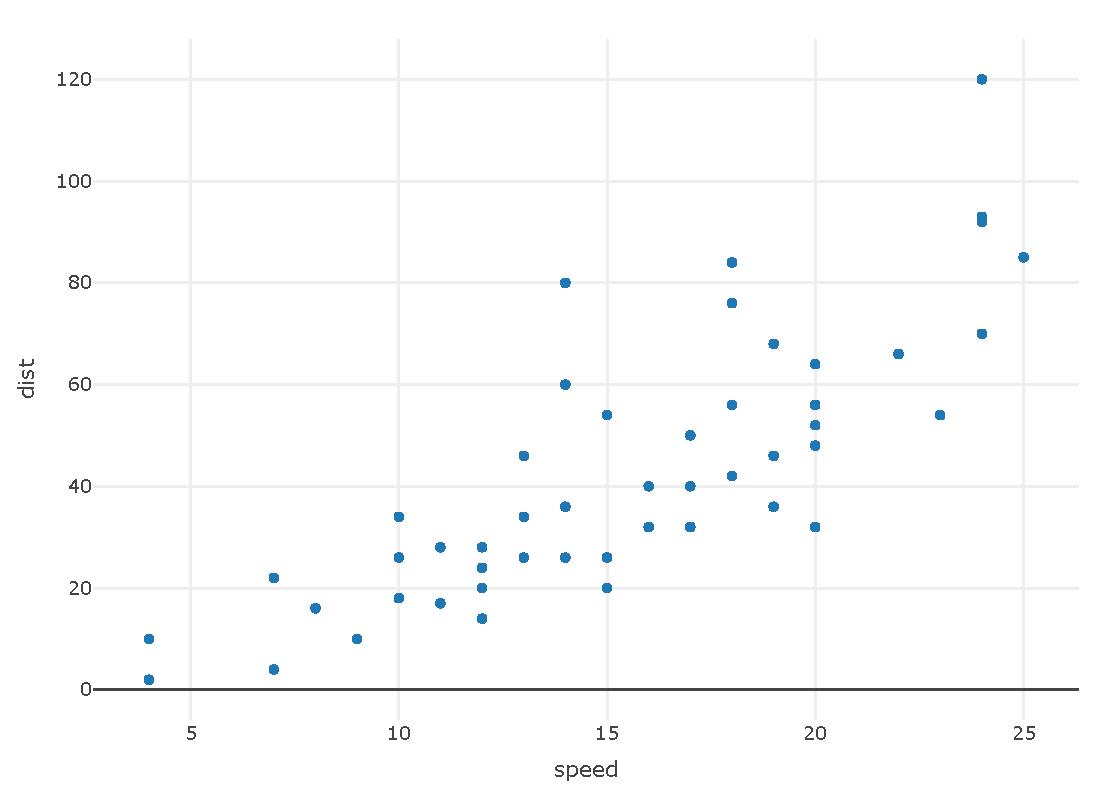
\includegraphics[width=0.9\linewidth]{logs/plotly-plot.pdf}
\begin{flushleft}
\end{flushleft}
\end{figure}
\vspace{-1.2cm}

\hypertarget{python}{%
\section{Python}\label{python}}

\hypertarget{api-data-download-using-python}{%
\subsection{API data download using Python}\label{api-data-download-using-python}}

\begin{Shaded}
\begin{Highlighting}[]
\ImportTok{import}\NormalTok{ sys}
\BuiltInTok{print}\NormalTok{(sys.version)}
\end{Highlighting}
\end{Shaded}

\begin{verbatim}
3.9.4 (tags/v3.9.4:1f2e308, Apr  6 2021, 13:40:21) [MSC v.1928 64 bit (AMD64)]
\end{verbatim}

\begin{Shaded}
\begin{Highlighting}[]
\ImportTok{import}\NormalTok{ json}
\CommentTok{\#\#from json.decoder import JSONDecodeError}
\ImportTok{import}\NormalTok{ requests}
\ImportTok{import}\NormalTok{ numpy }\ImportTok{as}\NormalTok{ np}
\ImportTok{import}\NormalTok{ pandas }\ImportTok{as}\NormalTok{ pd}

\CommentTok{\#\# INE: https://www.ine.pt/ine/json\_indicador/pindica.jsp?}
\CommentTok{\#\# op=2\&varcd=0008074\&Dim1=S7A2015\&Dim2=200\&Dim3=3\&lang=PT}

\CommentTok{\# api{-}endpoint}

\NormalTok{URL }\OperatorTok{=} \StringTok{"https://www.ine.pt/ine/json\_indicador/pindica.jsp"}

\CommentTok{\# define parameters}

\NormalTok{OP}\OperatorTok{=}\StringTok{"2"}
\NormalTok{VARCD}\OperatorTok{=}\StringTok{"0008074"}
\NormalTok{DIM1}\OperatorTok{=}\StringTok{"S7A2015"}
\NormalTok{DIM2}\OperatorTok{=}\StringTok{"200"}
\NormalTok{DIM3}\OperatorTok{=}\StringTok{"3"}
\NormalTok{LANG}\OperatorTok{=}\StringTok{"PT"}


\CommentTok{\# defining a params dict for the parameters to be sent to the API}
\NormalTok{PARAMS }\OperatorTok{=}\NormalTok{ \{}\StringTok{\textquotesingle{}op\textquotesingle{}}\NormalTok{:OP,}\StringTok{\textquotesingle{}varcd\textquotesingle{}}\NormalTok{:VARCD,}\StringTok{\textquotesingle{}Dim1\textquotesingle{}}\NormalTok{:DIM1,}\StringTok{\textquotesingle{}Dim2\textquotesingle{}}\NormalTok{:DIM2,}\StringTok{\textquotesingle{}Dim3\textquotesingle{}}\NormalTok{:DIM3,}\StringTok{\textquotesingle{}lang\textquotesingle{}}\NormalTok{:LANG\}}

\CommentTok{\# sending get request and saving the response as response object}
\NormalTok{r }\OperatorTok{=}\NormalTok{ requests.get(url }\OperatorTok{=}\NormalTok{ URL,params}\OperatorTok{=}\NormalTok{PARAMS)}

\CommentTok{\# extracting data in json format}
\NormalTok{data }\OperatorTok{=}\NormalTok{ r.json()}

\NormalTok{valor }\OperatorTok{=}\NormalTok{ data[}\DecValTok{0}\NormalTok{][}\StringTok{\textquotesingle{}Dados\textquotesingle{}}\NormalTok{][}\StringTok{\textquotesingle{}2015\textquotesingle{}}\NormalTok{][}\DecValTok{0}\NormalTok{][}\StringTok{\textquotesingle{}valor\textquotesingle{}}\NormalTok{]}

\NormalTok{valor}
\end{Highlighting}
\end{Shaded}

\begin{verbatim}
'1.8'
\end{verbatim}

The criminal rate is 1.8\%o.

\vspace{0.3cm}

\hypertarget{import-data-from-pdf-files}{%
\subsection{Import data from PDF files}\label{import-data-from-pdf-files}}

\begin{Shaded}
\begin{Highlighting}[]
  \BuiltInTok{cd}\NormalTok{ C:/Users/mangelo.EEG/Documents/GitHub/prjs/pdfs}
    \FunctionTok{find}\NormalTok{ . }\AttributeTok{{-}name} \StringTok{\textquotesingle{}*.pdf\textquotesingle{}} \AttributeTok{{-}print0} \KeywordTok{|} \FunctionTok{xargs} \AttributeTok{{-}0} \AttributeTok{{-}n1}\NormalTok{ pdfsandwich }\AttributeTok{{-}gray}
    \FunctionTok{find}\NormalTok{ . }\AttributeTok{{-}name} \StringTok{\textquotesingle{}*ocr.pdf\textquotesingle{}} \AttributeTok{{-}print0} \KeywordTok{|} \FunctionTok{xargs} \AttributeTok{{-}0} \AttributeTok{{-}n1}\NormalTok{ pdftotext}
\end{Highlighting}
\end{Shaded}

\begin{verbatim}
['ORNALOFICIAL', 'Tercḃa-feira, 2 de julho de 2019', '', 'IDY', 'Série', 'Numero 30', '', 'Sumario', 'VICE-PRESIDENCIA DO GOVERNO REGIONAL GREENMECHANICS, LDA.', 'Revogacao n.Ḟ 127/2019 Revogaa autorizagao concedida pelo entaéo Secretario Regional do Plano e Finangas em 24 de julho de 2012. GREENMECHANICS, LDA. & COMANDITA Revogacao n.Ḟ 128/2019 Revogaa autorizagao concedida pelo entéo Secretario Regional do Plano e Finangas em 24 de julho de 2012.', '', 'EXOMAR TRADING, LDA.', 'Revogacao n.Ḟ 129/2019 Revoga a autorizacao concedida pelo Vice-Presidente do Governo Regional em 24', '', 'de outubro de 2018. MILCA -- SERVICOS DE CONSULTORIA, TRADING, LDA.', 'Revogacaon.Ḟ 130/2019 Revoga a autorizacao concedida pelo entaéo Secretario Regional das Finangas e da Administragao Publica em 21 de agosto de 2017. Declaracaoderetificacao n.Ḟ 4/2019 Procede4 retificagao do n.Ḟ de contribuinte constante da Revogacao n.Ḟ 102/2019, de 5 de junho, da sociedade denominada SAGAMORE SERVICES, UNIPESSOAL, LDA., publicada no Jornal Oficial, IV Série, n.Ḟ 19, de 5 de junho de 2019. CONSERVATORIA DO REGISTO COMERCIAL E CARTORIO NOTARIAL PRIVATIVOS DA ZONA FRANCA DA MADEIRA Declaracaoderetificacao n.Ḟ 5/2019 Procede a retificacao da publicagéo respeitante a sociedade denominada MOOSEWIN - IT SOLUTIONS, UNIPESSOAL, LIMITADA a qual consta do Jornal Oficial, IV Série, n.Ḟ 21, de 12 de junho de 2019. ATLANTIC YARDS- SHIPYARDS MANAGEMENT, LDA. ConstituigAéo de sociedade e designacg4o de membrosde org4osocial Constituicao de sociedade por quotas e designacao de gerentes BALMWARD- CONSULTORIAE SERVICOS, UNIPESSOAL, LDA. Constituigaéo de sociedade e designac4o de membro de 6rg4osocial Constituicao de sociedade por quotas e designacao de gerente', '', 'BOM JESUS TANKERS, UNIPESSOAL,S.A.', 'Alteracao de Contrato de Sociedade Aditamento de um novoartigo 7.Ḟ - Prestagdes Acessorias de Capital e renumeraca de Artigos posteriores CANJALA TANKERS, UNIPESSOAL,S.A. Alteracao de Contrato de Sociedade Aditamento de um novoartigo 7.Ḟ - Prestagdes Acessorias de Capital e renumeraca de Artigos posteriores', '', '', 'IV Numero 30 CAPITOLES, LDA. Transformacao Transformacao em sociedade por quotas', '', '2 de julho de 201 © Juino ae ?', '', 'ERBOZETA IBERICA, UNIPESSOAL, LDA.', 'Constituicgdo de sociedade e designac4o de membrode orgaosocial Constituicao de sociedade por quotas e designacao de gerente ESARGROUP, LDA. Alteracao de Contrato de Sociedade Alteracao de Artigo 5.Ḟ - Capital Social FI - FSI1V, UNIPESSOAL,S.A. Alteracao de Contrato de Sociedade Aditamento de um novoartigo 7.Ḟ - Prestagdes Acessérias de Capital e renumeragao de Artigos posteriores', '', 'FINTEF, UNIPESSOAL, LDA.', 'Constituicgéo de sociedade e designac4o de membrode orgaosocial Constituicao de sociedade por quotas e designacao de gerente FINTEF, UNIPESSOAL, LDA. Alteracgao de Contrato de Sociedade e designacg4o de membrode 6rgaosocial Alteragao de alinea a) do n.Ḟ 4 do Artigo 9.Ḟ - Forma de Obrigar e designagaéo de', 'gerentes', '', 'FRECAJ - EMPRESA DE TRABALHO TEMPORARIO,LDA.', 'Constituicgéo de sociedade e designac4o de membrode orgaosocial Constituicao de sociedade por quotas e designacao de gerente FREETRADING - COMERCIO INTERNACIONAL E SERVICOS, LDA. Alteracao de Contrato de Sociedade Alteragao de Artigo 2.Ḟ - Objeto FULL BLOSSOM- TRADING E SERVICOS, SOCIEDADE UNIPESSOAL, LDA. Cessacao de funcdes de membro deorgaosocial Renuncia de gerente', '', 'GETVERIFY, LDA.', 'Constituicgéo de sociedade e designac4o de membrosde orgiosocial Constituicao de sociedade por quotas e designacao de gerentes ILHA BELA - GESTAO E TURISMO UNIPESSOAL, LDA. Cessacao de funcdes de membrode orgaosocial Renuncia de gerente ILHA BELA - GESTAO E TURISMO UNIPESSOAL, LDA. Cessacao de funcdes de membrode orgaosocial Renuncia de gerente ILHA BELA - GESTAO E TURISMO UNIPESSOAL, LDA. Designagao de membrosde 6rgaosocial Designagao de gerentes', '', 'JADAMA CORPORATION, LDA.', 'Constituicgéo de sociedade e designac4o de membrosde orgiosocial Constituicao de sociedade por quotas e designacao de gerentes JAN DE NUL PORTUGAL, LDA. Designacéo de membrode 6rgaosocial - Atualizacao Designagao de gerente JAPAFRICA MOBILITY SOLUTIONS, UNIPESSOAL, LDA. Aumento do Capital Social, alteragao de Contrato de Sociedade e designacAo de membrode 6rgaosocial Montante do aumento: 500 000,00 Euros; Alteragéo de 1.Ḟ - Denominagao, 2.Ḟ - Objeto, 3.Ḟ - Capital e 4.Ḟ - Forma De Obrigar e eliminacgao do artigo 5.Ḟ e designagao de gerentes', '', 'M2IS - MADEIRA INTERNATIONAL SOLUTIONS,S.A.', 'Aumento do Capital Social e alterag4o de Contrato de Sociedade Montante do aumento: 25.000,00 Euros e Alteragao de Artigo 5.Ḟ - Capital Social MADPROFIT V, UNIPESSOAL, LDA. Cessacao de funcdes de membrode orgaosocial Renuncia de gerente', '', '', '2 de julho de 2019', '', 'Ty', 'Numero 30 MADPROFIT V, UNIPESSOAL, LDA. Designacgao de membro de 6rgaosocial Designagao de gerente NEWMETALDEV (TRADING) - CONSULTADORIA E SERVICOS, UNIPESSOAL, LDA. Alteracao de Contrato de Sociedade Alteracao de Artigo 4.Ḟ - Capital OMMIACREST TRADING, LDA. Cessacao de funcdes de membrode orgaosocial Renuncia de gerente OMMIACREST TRADING, LDA. Cessacao de funcdes de membrode orgaosocial Renuncia de gerente OMMIACREST TRADING, LDA. Designacéo de membrode 6rgaosocial Designagao de gerente PERUN SHIPPING, LDA. Cessacao de funcdes de membrode orgaosocial Exoneragao de gerente PERUN SHIPPING, LDA. Designacéo de membrode 6rgaosocial Designagao de gerente PJS HOLDING CORP,S.G.P.S., LDA. Constituigéo de sociedade e designac4o de membrosde 6rgaossociais Constituicgao de sociedade por quotas, designacdo de gerentes e de Revisores Oficias de Contas Efetivo e Suplente QTT PORTUGAL, UNIPESSOAL, LDA. Designacéo de membro de 6rgaosocial Designagao de gerente', '', 'RICH HILL, S.G.P.S., LDA.', 'Mudanga Mudanga de ambito para fora da Zona Franca', '', 'SERLIMAWASH - LAVANDARIA INDUSTRIAL,S.A.', 'Designac4o de membrosde 6rgiosocial Designagao de Fiscais Unico Efetivo e Suplente SORBITOL - COMERCIO INTERNACIONALE SERVICOS, LDA. Cessacao de funcées de membrosde orgaosocial Exoneracao de gerentes SORBITOL - COMERCIO INTERNACIONALE SERVICOS, LDA. Designacéo de membro de 6rgaosocial Designagao de gerente SORBITOL - COMERCIO INTERNACIONALE SERVICOS, LDA. Mudanga de sede Sede: Rua Ponta da Cruz - Funchal SOUTH ESSENCE, LDA. Aumento do Capital Social, alterag4o de Contrato de Sociedade e designacAo de membro de 6rgaosocial- Retificagao Montante do aumento: 9.000,00 Euros; Alteragéo de Artigos 2.Ḟ, n.Ḟ 1 - Sede; 6.Ḟ - Capital Social e 13.Ḟ, n.Ḟ 2 - Forma de Obrigar e designacao de gerente SUFFOLKS.G.P.S., SOCIEDADE UNIPESSOAL,S.A. Transformacao e alterag4o de Contrato de Sociedade Transformacao em Sociedade Unipessoal e alteragao de Artigos 1.Ḟ - Denominagao e n.Ḟ | do 6.Ḟ - Acdes WALKING BACK THECAT, LDA. Alteracao de Contrato de Sociedade Alteragao de Artigos 1.Ḟ - Denominagao e 2.Ḟ - Objeto', '', 'WILLIWAW HUB, UNIPESSOAL, LDA.', 'Constituigdo de sociedade e designac4o de membrode orgaosocial Constituicao de sociedade por quotas e designacao de gerente', '', '', 'Numero 30 VICE-PRESIDENCIA DO GOVERNO REGIONAL GREENMECHANICS, LDA.', 'Revogacao n.Ḟ 127/2019 NIPCe matricula: 510 340 989; Sede social: Rua Ivens, n.Ḟ 3, Edificio Dona Mécia,n.Ḟ 6, Funchal ZONA FRANCA DA MADEIRA', '', '2 de julho de 2019', '', 'Declaracao de retificacao n.Ḟ 4/2019', '', 'Por ter sido publicado com inexatidio o NIPC da sociedade "SAGAMORE SERVICES, UNIPESSOAL, LDA", na revogagio n.Ḟ 102/2019, publicada no JORAM IV série, n.Ḟ 19 de 5 de junho de 2019:', 'Ondese lé.:', '', '"SAGAMORE SERVICES, UNIPESSOAL, LDA."', 'NIPC E MATRICULA:514 422 874." Develer-se "SAGAMORE SERVICES, UNIPESSOAL, LDA." NIPC E MATRICULA: 514 228 874"', '', 'Torna-se publico que por despacho de Sua Exceléncia o Vice-Presidente do Governo Regional de 2019.06.07, foi revogada a autorizagao concedida pelo entdo Secretario Regional do Plano e Finangas em 24.07.2012, para o exercicio da atividade da sociedade', '"GREENMECHANICS, LDA.".', '', 'Vice-Presidéncia do Governo Regional da Madeira, a 12 de junho de 2019.', 'O CHEFE DE GABINETE, Luis Nuno Olim', '', 'Vice-Presidéncia do Governo Regional da Madeira, aos 13 de junho de 2019.', 'O CHEFE DE GABINETE, Luis Nuno Olim', '', 'GREENMECHANICS, LDA. & COMANDITA', 'Revogacao n.Ḟ 128/2019 NIPCe matricula: 510 342 426; Sede social: Rua Ivens, n.Ḟ 3, Edificio Dona Mécia,n.Ḟ 6, Funchal ZONA FRANCA DA MADEIRA', '', 'CONSERVATORIA DO REGISTO COMERCIAL E CARTORIO NOTARIAL PRIVATIVOS DA ZONA FRANCA DA MADEIRA', 'Declaracdo deretificacao n.Ḟ 5/2019', '', 'Maria de Fatima Pereira dos Reis Coelho, Conservadora do Registo', 'Comercial e Cartério Notarial Privativos da Zona Franca da Madeira, informa que a publicacéo de Constituigéo de Sociedade denominada:', '', 'Torna-se publico que por despacho de Sua Exceléncia o Vice-Presidente do Governo Regional de 2019.06.07, foi revogada a autorizagao concedida pelo entdo Secretario Regional do Plano e Finangas em 24.07.2012, para o exercicio da atividade da sociedade', '"GREENMECHANICS, LDA. & COMANDITA".', '', '"MOOSEWIN -- IT SOLUTIONS, UNIPESSOAL LIMITADA", N.LP.C.: 515 445 525, publicada no JORAM n.Ḟ 21 do dia 12-06-2019, foi indevidamente remetida para publicagéo, uma vez que o seu registo foi efetuado provisoriamente por dividas, por nao ter apresentado licenca para poder operar no 4mbito da Zona Franca da Madeira, pelo que se da sem efeito aquela. Funchal, 14 de junho de 2019. A CONSERVADORA, Maria de Fatima Pereira dos Reis Coelho ATLANTIC YARDS - SHIPYARDS MANAGEMENT,LDA.', 'Para efeitos de Publicagao - Maria Isabel Velosa Barreto Ferreira Alves, Oficial de Registos,', '', 'Vice-Presidéncia do Governo Regional da Madeira, a 12 de junho de 2019.', 'O CHEFE DE GABINETE, Luis Nuno Olim', '', 'EXOMAR TRADING,LDA. Revogagao n.Ḟ 129/2019', 'NIPCe matricula: 515 070 319; Sede social: Rua da Alfandega, n.Ḟ 78, 3Ḟ Andar, 9000-059 Funchal ZONA FRANCA DA MADEIRA', '', 'Certifica/Publica que: Em relagéo 4 entidade: N.Ḟ de Matricula/NIPC: 9084) Natureza Juridica: SOCIEDADE POR QUOTAS', 'Sede:', '', '515485969 (Pasta n.Ḟ', '', 'Torna-se putblico que por despacho de Sua Exceléncia o Vice-Presidente do Governo Regional de 2019/06/07 foi revogada a autorizagao concedida pelo mesmo em 2018/10/24, para o exercicio da', 'atividade da sociedade "EXOMAR TRADING, LDA."', '', 'Firma: ATLANTIC YARDS - SHIPYARDS MANAGEMENT, LDA. (ZONA FRANCA DA MADEIRA) Rua dos Murgas, n.Ḟ 15, 1.Ḟ andar Distrito: Ilha da Madeira', '', 'Concelho: Funchal Freguesia: Funchal (Sé) 9000-058 Funchal', 'Pela Apresentagaéo AP. 4/20190611, referente 4 inscrigao 1, foi efetuado o', '', 'Vice-Presidéncia do Governo Regional da Madeira, a 12 de junho de 2019.', 'O CHEFE DE GABINETE, Luis Nuno Olim', '', 'seguinte ato de registo: . Insc. 1 - AP. 4/20190611 12:31:14 UTC - CONSTITUIGAO DE', '', 'SOCIEDADE E DESIGNACAO DE MEMBRO(S) DE ORGAO(S)', '', 'MILCA -- SERVICOS DE CONSULTORIA, TRADING, LDA. Revogagao n.Ḟ 130/2019', 'NIPCe matricula: 514 518 170; Sede social: Rua dos Murgas, n.Ḟ 15, 3Ḟ Andar, Sala L, 9000-058 Funchal ZONA FRANCA DA MADEIRA', '', 'SOCIAL(AIS)', 'FIRMA: ATLANTIC YARDS - SHIPYARDS MANAGEMENT,LDA. (ZONA FRANCA DA MADEIRA)', '', 'NIPC: 515485969', 'NATUREZA JURIDICA: SOCIEDADE POR QUOTAS Sede: Rua dos Murgas, n.Ḟ 15, 1.Ḟ andar Distrito: Ilha da Madeira', '', 'Concelho: Funchal Freguesia: Funchal (Sé) 9000-058 Funchal OBJETO:1. Consultoria Técnica, a gestao manutengao e desenvolvimento de estaleiros navais; 2. Corretagem comercial; 3. Consultoria para a', 'reparagdo e manutengao de todo o tipo de embarcagées e infraestruturas', '', 'Torna-se publico que por despacho de Sua Exceléncia o Vice-Presidente do Governo Regional de 2019.06.11, foi revogada a autorizagao concedida pelo entéo Secretario Regional das Finangas e da Administragéo Piblica em 21.08.2017, para o exercicio da atividade da sociedade "MILCA -- SERVICOS DE CONSULTORIA, TRADING,', 'LDA.".', '', 'maritimas; 4. Compra e venda de todo o tipo de materiais, maquinas,', 'servigos e equipamentos; 5. Prestagao de servigos maritimos; 6. Selegao,', '', 'recrutamento e desenvolvimento de carreiras. CAPITAL:5.000,00 Euros', 'Montante realizado: 0,00 Euros', '', 'Data de Encerramento do Exercicio: 31 dezembro', '', 'Vice-Presidéncia do Governo Regional da Madeira, a 12 de junho de 2019.', 'O CHEFE DE GABINETE, Luis Nuno Olim', '', 'SOCIOS E QUOTAS:', '', 'QUOTA:4.500,00 Euros', '', 'MADEIRA)', '', 'TITULAR:', '', 'FAMAR', '', 'OFFSHORE,', '', 'S.A.', '', '(ZONA', '', 'FRANCA', '', 'DA', '', '', '2 de julho de 2019', '', 'Numero 30 exploragao de direitos de propriedade intelectual e industrial, nomeadamente, de marcas registadas, patentes e direitos de autor e direitos conexos. O comércio por grosso e a retalho de todo o tipo de matérias primas, produtos, artigos e bens de consumo, sem especializacéo. Atividades imobilidrias, nomeadamente a compra de imdveis para revenda e as atividades de arrendamento e exploragao de bens imobilidrios. O alojamento mobiliado para turistas. A gestéo da carteira propria de titulos, nomeadamente quaisquer instrumentos financeiros e valores mobilidrios, bem como aplicagdes financeiras; comissdes e consignacGes.', 'CAPITAL: 100,00 Euros', '', 'NIF/NIPC: 513645705', 'Residéncia/Sede: Rua dos Murgas, n.Ḟ 15, 1.Ḟ andar 9000-058 Funchal', '', 'QUOTA:500,00 Euros', 'TITULAR: MAURO DOS SANTOS BATALHA DE CARVALHO', '', 'NIF/NIPC: 276823338 Estado civil: Solteiro(a) maior', 'Residéncia/Sede: Rua Nicolau G Spencer, n.Ḟ 6, R/C, Bairro Maculusso,', '', 'Ingombotas Angola', '', 'FORMA DE OBRIGAR/ORGAOSSOCIAIS:', 'Forma de obrigar: a) Assinatura de qualquer UM dos gerentes (independentemente do grupo a que pertencam), em atos de administragao ordinaria, até o montante maximo de mil euros por transacao; b) Assinatura de UM gerente do grupo A, em atos de administracao ordinaria, acima do montante maximo de mil euros por transac4o; c) Assinatura de UM gerente de qualquer um dos grupos A ou B, desde que previamente autorizado e assembleia geral de sdcios; d) Assinatura de um mandatario ou procuradorda sociedade com poderes delegados. Estrutura da geréncia: Pertence a DOIS ou MAISgerentes, divididos em dois grupos: Ae B.', 'DECLARACAO RELATIVA AO CAPITAL:Ossécios comprometem-se,', '', '.', '', 'Data de Encerramento do Exercicio: 31 dezembro', '', 'SOCIOS E QUOTAS:', '', 'QUOTA:100,00 Euros', 'TITULAR: CRUSADE TRUST ADMINISTRATORS (NAMIBIA)', '', '(PROPRIETARY) LIMITED - que atua na qualidade de TRUSTEE do', 'trust "FORRO DE PRATA TRUST"', '', 'NIF/NIPC: 980626072', 'Residéncia/Sede: CRVW POBOX 97401, Maerua Mall, Windhoek', '', 'até ao final do ano civil, a depositar o valor das respetivas entradas em conta bancaria aberta em nomeda sociedade. ORGAO(S) DESIGNADO(S): GERENCIA:', 'Nome/Firma: MAURO DOS SANTOS BATALHA DE CARVALHO', '', 'Namibia TITULAR: INGRID DAWN STADLER - que atua na qualidade de', 'TRUSTEEdotrust "FORRO DE PRATA TRUST"', '', 'NIF/NIPC: 276823338', 'Cargo: Gerente - Grupo A Residéncia/Sede: Rua Nicolau G Spencer, n.Ḟ 6, R/C, Bairro Maculusso,', '', 'NIF/NIPC: 297922963 Estadocivil: Divorciado(a) Residéncia/Sede: 395 Soetdoring Street Finkentein Village Windhoek Namibia .', '', 'FORMA DE OBRIGAR/ORGAOSSOCIAIS:', '', 'Ingombotas Angola Nome/Firma: LUIS CRISTIANO VIEIRA MOTA NIBF/NIPC: 218981759', 'Cargo: Gerente - Grupo B Residéncia/Sede: Rua dos Murgas, n.Ḟ 15, 1.Ḟ andar Funchal Data da deliberagdo: 11-06-2019', '', 'Entidade com os documentos integralmente depositados em suporte eletrénico. Conservatoria do Registo Comercial ḃ Cartério Notarial Privativos da Zona Franca da Madeira, aos 12 de junho de 2019.', 'O OFICIAL DE REGISTOS, Maria Isabel V.B. Ferreira Alves', '', 'Forma de obrigar: Assinatura de QUALQUERdosseusgerentes. Estrutura da geréncia: Pertence a UM ou MAISgerentes. O trust: "FORRO DE PRATA TRUST" com o NIF 770 010 865, foi constituido segundoasleis da Republica da Namibia, esta depositado junto ao Master of High Court,em Windhoek, e registado sob o nimero T131/18. A gestao e representagao do Trust pertence aos dois TRUSTEES acimaidentificados. ORGAO(S) DESIGNADO(S): GERENCIA:', 'Nome/Firma: ROBERTO CARLOS DE CASTRO ABREU', '', 'NIF/NIPC: 202559815', 'Cargo: Gerente Residéncia/Sede: Avenida do Infante, n.Ḟ 8, Edificio Executivo, 2.Ḟ andar, sala K, Sé 9000-015 Funchal Data da deliberagdo: 13-06-2019', '', 'BALMWARD - CONSULTORIA E SERVICOS, UNIPESSOAL, LDA.', 'Para efeitos de Publicagao - Ana Maria Gongalves Ferreira Carvalho, Oficial de Registos,', '', 'O(s) documento(s) que serviu(ram) de base ao presente registo encontra(m)-se depositado(s) na pasta eletronica da Sociedade. Funchal, 21 de junho de 2019', 'OFICIAL DE REGISTOS, Ana Maria Gongalves Ferreira Carvalho', '', 'Certifica que: Publica-se que em relagao a entidade: N.Ḟ de Matricula/NIPC: 515517135 (Pasta n.Ḟ 9092) Firma: BALMWARD - CONSULTORIA E SERVICOS, UNIPESSOAL,', 'LDA. (ZONA FRANCA DA MADEIRA) Natureza Juridica: SOCIEDADE POR QUOTAS Sede: Avenida do Infante, n.Ḟ 8, Edificio Executivo, 2.Ḟ andar, sala K', '', 'BOM JESUS TANKERS, UNIPESSOAL,S.A.', 'Para efeitos de Publicagao - Maria Isabel Velosa Barreto Ferreira Alves, Oficial de Registos,', '', 'Distrito: Ilha da Madeira Concelho: Funchal Freguesia: Funchal (Sé) 9000-015 Funchal', 'Pela Apresentagao AP. 1/20190621, referente a inscrigado 1, foi efetuado o', '', 'Certifica que: Publica-se que em relag&o a entidade: N.Ḟ de Matricula/NIPC: 515092550 (Pasta n.Ḟ 8982) Firma: BOM JESUS TANKERS, UNIPESSOAL,S.A. (ZONA FRANCA', '', 'seguinte ato de registo: . Insc. 1 - AP. 1/20190621 10:43:25 UTC - CONSTITUICAO DE', '', 'Natureza Juridica: SOCIEDADE ANONIMA', 'Sede: Rua dos Murgas, n.Ḟ 15, 1.Ḟ andar Distrito: Ilha da Madeira', '', 'DA MADEIRA)', '', 'SOCIEDADE E DESIGNACAO DE MEMBRO(S) DE ORGAO(S)', '', 'Concelho: Funchal Freguesia: Funchal (Sé) 9000-058 Funchal', 'Pela Apresentagao AP. 6/20190612,referente a inscrigao 2, foi efetuado o', '', 'SOCIAL(AIS)', 'FIRMA: BALMWARD CONSULTORIA E UNIPESSOAL, LDA. (ZONA FRANCA DA MADEIRA)', '', 'SERVICOS,', '', 'seguinte ato de registo:', 'Insc. 2 - AP. 6/20190612 11:41:48 UTC CONTRATO DE SOCIEDADE - ALTERACOES AO .', '', 'NIPC: 515517135 |', 'NATUREZA JURIDICA: SOCIEDADE POR QUOTAS SEDE: Avenida do Infante, n.Ḟ 8, Edificio Executivo, 2.Ḟ andar, sala K', '', 'Distrito: Ilha da Madeira Concelho: Funchal Freguesia: Funchal (Sé) 9000-015 Funchal', 'OBJETO: A prestagao de servigos de consultoria econédmica e de contabilidade; a prestagao de servigos de planeamento, organizacao, controlo, informagao e gest4o e administracao; A atividade de escritérios de comiss6es, consignacdes e', '', 'Artigo(s) alterado(s): Aditamento de um novoartigo 7.Ḟ PRESTACOES ACESSORIAS DE CAPITAL), renumerando em consequénciaosartigos posteriores. Os documentos que serviram de base ao presente registo estao depositados em suporte eletrénico. Conservatoria do Registo Comercial da Zona Franca da Madeira, aos 12 de junho de 2019.', 'OFICIAL DE REGISTOS, Maria Isabel Velosa Barreto Ferreira Alves', '', 'agenciamento comercial dessas mercadorias, bem comoa prestacao de servicos de consultoria econdmica, marketing e publicidade. A prestacdo de servigos de', 'consultoria de informatica e atividades conexas, como prestagao de servigos na', '', 'Internet. A aquisigaéo, venda, agenciamento e qualquer outra forma de', '', '', 'Ty', 'Numero 30 CANJALA TANKERS, UNIPESSOAL,S.A.', 'Para efeitos de Publicagao - Jacinta Iria Andrade', '', '2 de julho de 2019', '', 'NIPC: 515522988 |', 'NATUREZA JURIDICA: SOCIEDADE POR QUOTAS Sede: Edificio Marina Club, Avenida Arriaga, n.Ḟ 73, 1.Ḟ, sala 105Distrito:', '', 'Drumond, Oficial de Registos, Certifica que: Publica-se que em relagao a entidade: N.Ḟ de Matricula/NIPC: 515092649 (Pastan.Ḟ 8976) Firma: CANJALA TANKERS, UNIPESSOAL, S.A. (ZONA FRANCA', '', 'Ilha da Madeira Concelho: Funchal Freguesia: Funchal (Sé) 9004-533 Funchal OBJETO:ComissGes, consignagées e representagdes de produtos, bem como a', 'sua comercializacao, incluindo importagao e exportacao; Comércio por grosso', '', 'de bens de consumo, nomeadamente suplementos alimentares, dispositivos médicos e cosméticos; Consultadoria para os negécios e outra consultoria', 'para a gesto.', '', 'Natureza Juridica: SOCIEDADE ANONIMA', 'Sede: Rua dos Murgas, n.Ḟ 15, 1.Ḟ andar Distrito: Ilha da Madeira', '', 'DA MADEIRA)', '', 'CAPITAL: 10.000,00 Euros', 'Montante realizado: 0,00 Euros', '', 'Concelho: Funchal Freguesia: Funchal (Sé) 9000-058 Funchal', 'Pela Apresentagao AP. 11/20190612,referente 4 inscricao 2, foi efetuado', '', 'Data de Encerramento do Exercicio: 31 dezembro', '', 'SOCIOS E QUOTAS:', '', 'QUOTA:10.000,00 Euros', 'TITULAR: ERBOZETAS.P.A.', '', '0 seguinte ato de registo: . Insc. 2 - AP. 11/20190612 14:55:49 UTC - ALTERACOES AO', 'CONTRATO DE SOCIEDADE .', '', 'NIF/NIPC: 980650380', 'Residéncia/Sede: Strada delle Seriole, 41/43, 47894 Chiesanuova', '', 'Artigo(s) alterado(s): Aditamento de um novoartigo 7.Ḟ (PRESTACOES ACESSORIAS DE CAPITAL) e em consequéncia renumeram osartigos seguintes. O(s) documento(s) que serviu(ram) de base ao presente registo encontra(m)-se depositado(s) na pasta eletronica da Sociedade. Funchal, 12 de junho de 2019.', 'OFICIAL DE REGISTOS, Jacinta Iria Andrade Drumond', '', 'Republica de San Marino', '', 'FORMA DE OBRIGAR/ORGAOSSOCIAIS:', 'Formade obrigar: Assinatura de qualquer UM dos seus gerentes -OU- de mandatario ou procurador, com poderes conferidos. Estrutura da geréncia: Pertence a UM ou MAISgerentes. DECLARACAO RELATIVAAO CAPITAL: O sécio inico comprometese a realizar até final do primeiro exercicio econdmico, o valor da respetiva entrada. ORGAO(S) DESIGNADO(S): GERENCIA:', 'Nome/Firma: ROBERTO ZAVAGLIA', '', '.', '', 'NIF/NIPC: 299659917 CAPITOLES, LDA.', 'Para efeitos de Publicagao - Ana Maria Gongalves Ferreira Carvalho, Oficial de Registos, Cargo: Gerente', '', 'Residéncia/Sede: Via del Camerario 67, 47891 Republica de San Marino', 'Data da deliberagdo: 12-06-2019', '', 'Certifica que: Publica-se que em relagao a entidade: N.Ḟ de Matricula/NIPC: 514532718 (Pasta n.Ḟ 8755)', 'Firma: CAPITOLES, LDA. (ZONA FRANCA DA MADEIRA) Natureza Juridica: SOCIEDADE POR QUOTAS', '', 'Entidade com os documentos integralmente depositados em suporte eletrénico. Conservatoria do Registo Comercial da Zona Franca da Madeira, aos 13 de junho de 2019.', 'OFICIAL DE REGISTOS, Maria Isabel Velosa Barreto Ferreira Alves', '', 'Sede: Rua da Carreira n.Ḟ 102 Distrito: Ilha da Madeira Concelho: Funchal Freguesia: Funchal (Sao Pedro) 9000-042 Funchal', 'Pela Apresentagao AP. 4/20190618, referente a inscricdo 3, foi efetuado o', '', 'ESARGROUP, LDA.', 'Para efeitos de Publicagdo - Ana Maria Gongalves Ferreira Carvalho, Oficial de Registos,', '', 'seguinte ato de registo: . Insc. 3 - AP. 4/20190618 14:59:32 UTC - TRANSFORMACAO DE', 'SOCIEDADE UNIPESSOAL EM SOCIEDADE POR QUOTAS FIRMA: CAPITOLES, LDA. (ZONA FRANCA DA MADEIRA)', '', 'NIPC: 514532718', 'NATUREZA JURIDICA: SOCIEDADE POR QUOTAS', '', 'Certifica que: Publica-se que em relagao a entidade: N.Ḟ de Matricula/NIPC: 510649068 (Pasta n.Ḟ 7985)', 'Firma: ESARGROUP, LDA. (ZONA FRANCA DA MADEIRA)', '', 'O(s) documento(s) que serviu(ram) de base ao presente registo encontra(m)-se depositado(s) na pasta eletrénica da Sociedade. Funchal, 19 de junho de 2019.', 'OFICIAL DE REGISTOS, Ana Maria Gongalves Ferreira Carvalho', '', 'Natureza Juridica: SOCIEDADE POR QUOTAS', 'Sede: Avenida Dom Teodoro de Faria, n.Ḟ 4, Bloco 1 - 5.Ḟ D Distrito: Ilha', '', 'da Madeira Concelho: Funchal Freguesia: Sao Martinho 9000-782 Funchal', 'Pela Apresentagao AP. 9/20190617,referente a inscrigao 5, foi efetuado o', '', 'seguinte ato de registo: . Insc. 5 - AP. 9/20190617 15:33:06 UTC - ALTERACOES AO ERBOZETAIBERICA, UNIPESSOAL, LDA.', 'Para efeitos de Publicagao - Maria Isabel Velosa Barreto Ferreira Alves, Oficial de Registos, CONTRATO DE SOCIEDADE', '', 'SOCIOS E QUOTAS:', '', 'QUOTA:3.500,00 Euros', 'TITULAR: NATALIA NICOLAEVNA KOVALEVA SEQUEIRA', '', 'Certifica que: Publica-se que em relagao a entidade: N.Ḟ de Matricula/NIPC: 515522988 (Pasta n.Ḟ 9086)', 'Firma: ERBOZETA IBERICA, UNIPESSOAL, LDA. (ZONA FRANCA DA MADEIRA)', '', 'NIBF/NIPC: 218222653 Estadocivil: Casado(a) Nomedo cénjuge: Manuel Francisco Sequeira Regime de bens: Separacao de bens', 'Residéncia/Sede: Calle Real 31, 2 b, Paracuellos de Jarama, 28860 Madrid', '', 'Natureza Juridica: SOCIEDADE POR QUOTAS', 'Sede: Edificio Marina Club, Avenida Arriaga, n.Ḟ 73, 1.Ḟ, sala 105 Distrito:', '', 'Espanha QUOTA:1.500,00 Euros', 'TITULAR: NATALIA NICOLAEVNA KOVALEVA SEQUEIRA', '', 'Ilha da Madeira Concelho: Funchal Freguesia: Funchal (Sé) 9004-533 Funchal', 'Pela Apresentagao AP. 8/20190612,referente a inscrigado 1, foi efetuado o', '', 'NIBF/NIPC: 218222653 Estadocivil: Casado(a) Nomedo cénjuge: Manuel Francisco Sequeira Regime de bens: Separacao de bens', 'Residéncia/Sede: Calle Real 31, 2 b, Paracuellos de Jarama, 28860 Madrid', '', 'seguinte ato de registo: . Insc. 1 - AP. 8/20190612 12:27:03 UTC - CONSTITUICAO DE', 'SOCIEDADE E DESIGNACAO DE MEMBRO(S) DE ORGAO(S)', '', 'Espanha Artigo(s) alterado(s): 5.Ḟ (CAPITAL SOCIAL) O(s) documento(s) que serviu(ram) de base ao presente registo encontra(m)-se depositado(s) na pasta eletronica da Sociedade.', '', 'SOCIAL(AIS)', 'FIRMA: ERBOZETA IBERICA, FRANCA DA MADEIRA) UNIPESSOAL, LDA.', '', '(ZONA', '', '', '2 de julho de 2019', '', 'Numero 30 servigos nas areas de informatica, do marketing, da publicidade, gest@o de imagem, de arquitetura urbana e industrial, o exercicio da atividade', 'industrial ḃ comercial de investimentos imobilidrios, designadamente, a compra, venda e revenda de bens imdveis, e a exploragao, gestdo,', '', 'Funchal, 18 de junho de 2019.', 'OFICIAL DE REGISTOS, Ana Maria Gongalves Ferreira Carvalho', '', 'FI - FSIV, UNIPESSOAL,S.A.', 'Para efeitos de Publicagao - Maria Isabel Velosa Barreto Ferreira Alves, Oficial de Registos,', '', 'administragao e arrendamento de imdéveis da sua propriedade ou de terceiros; a atividade de promogao, marketing e prospecgao de mercados para os géneros e servigos acima especificados.', 'CAPITAL: 5.000,00 Euros', '', 'Data de Encerramento do Exercicio: 31 dezembro', '', 'Certifica que: Publica-se que em relagao a entidade: N.Ḟ de Matricula/NIPC: 515080985 (Pasta n.Ḟ 8975)', 'Firma:', '', 'SOCIOS E QUOTAS:', '', 'QUOTA:5.000,00 Euros', 'TITULAR: ALESSANDRO BIANCHI', '', 'Natureza Juridica: SOCIEDADE ANONIMA', 'Sede: Rua dos Murgas, n.Ḟ 15, 1.Ḟ andar Distrito: Ilha da Madeira', '', 'MADEIRA)', '', 'FI', '', '-', '', 'FSIV,', '', 'UNIPESSOAL,', '', 'S.A.', '', '(ZONA FRANCA DA', '', 'Concelho: Funchal Freguesia: Funchal (Sé) 9000-058 Funchal', 'Pela Apresentagao AP. 5/20190612, referente 4 inscricdo 2, foi efetuado o', '', 'NIF/NIPC: 299602109 Estadocivil: Casado(a) Nomedo cénjuge: Giuseppina Piliego Regime de bens: Separacao de bens Residéncia/Sede: Via Degli Stradelli Gelfi, 28/4, 40138 Bolonha Italia', '', 'FORMA DE OBRIGAR/ORGAOSSOCIAIS:', 'Forma de obrigar: Assinatura de UM gerente. ORGAO(S) DESIGNADO(S): GERENCIA:', '', 'seguinte ato de registo:', 'Insc. 2 - AP. 5/20190612 11:40:23 UTC CONTRATO DE SOCIEDADE - ALTERACOES AO .', '', 'Estrutura da geréncia: Pertence a UM ou MAISgerentes.', '', '.', 'CANHA ORNELAS FRAZAO', '', 'Artigo(s) alterado(s): Aditamento de um novoartigo 7.Ḟ (PRESTACOES ACESSORIASDE CAPITAL), renumerando em consequéncia os artigos posteriores. Os documentos que serviram de base ao presente registo estao depositados em suporte eletrénico. Conservatoria do Registo Comercial da Zona Franca da Madeira, aos 12 de junho de 2019.', 'OFICIAL DE REGISTOS, Maria Isabel Velosa Barreto Ferreira Alves', '', 'Nome/Firma:', '', 'ROSA MARIA DE', '', 'AFONSO NIF/NIPC: 192579290', 'Cargo: Gerente Residéncia/Sede: Avenida Arriaga n.Ḟ 30, 1.Ḟ andar, sala A9000-064', '', 'Funchal', 'Data da deliberagdo: 17-06-2019', '', 'O(s) documento(s) que serviu(ram) de base ao presente registo encontra(m)-se depositado(s) na pasta eletronica da Sociedade. Funchal, 18 de junho de 2019.', 'OFICIAL DE REGISTOS, Ana Maria Gongalves Ferreira Carvalho', '', 'FINTEF, UNIPESSOAL, LDA.', 'Para efeitos de Publicagao - Ana Maria Gongalves Ferreira Carvalho, Oficial de Registos,', '', 'FINTEF, UNIPESSOAL, LDA.', 'Para efeitos de Publicagao - Jacinta Iria Andrade Drumond, Oficial de Registos,', '', 'Certifica que: Publica-se que em relagao a entidade: N.Ḟ de Matricula/NIPC: 515518565 (Pasta n.Ḟ 9089)', 'Firma:', '', 'MADEIRA)', '', 'FINTEF,', '', 'UNIPESSOAL,', '', 'LDA.', '', '(ZONA', '', 'FRANCA', '', 'DA', '', 'Natureza Juridica: SOCIEDADE POR QUOTAS', 'Sede: Avenida Arriaga n.Ḟ 30, 1.Ḟ andar, sala A Distrito: Ilha da Madeira', '', 'Certifica/Publica que: Em relacgéo a entidade: N.Ḟ de Matricula/NIPC: n.Ḟ (9089)', 'Firma:', '', '515518565 (Pasta', 'FRANCA DA', '', 'Concelho: Funchal Freguesia: Funchal (Sé) 9000-064 Funchal', 'Pela Apresentagao AP. 4/20190617, referente 4 inscricdo 1, foi efetuado o', '', 'MADEIRA)', '', 'FINTEF,', '', 'UNIPESSOAL,', '', 'LDA.', '', '(ZONA', '', 'Natureza Juridica: SOCIEDADE POR QUOTAS', 'Sede: Avenida Arriaga n.Ḟ 30, 1.Ḟ andar, sala A Distrito: Ilha da Madeira', '', 'seguinte ato de registo: Insc. 1 - AP. 4/20190617 11:51:05 UTC - CONSTITUICAQ DE', 'SOCIEDADE E DESIGNACAO DE MEMBRO(S) DE ORGAO(S)', '', 'Concelho: Funchal Freguesia: Funchal (Sé) 9000-064 Funchal', 'Pela Apresentagao AP. 1/20190619,referente a inscrigao 2, foi efetuado o', '', 'SOCIAL(AIS)', 'FIRMA:', '', 'MADEIRA)', '', 'FINTEF,', '', 'UNIPESSOAL,', '', 'LDA.', '', '(ZONA', '', 'FRANCA', '', 'DA', '', 'seguinte ato de registo: Insc. 2 - AP. 1/20190619 10:09:39 UTC - ALTERACOES AO', 'CONTRATO DE SOCIEDADE E DESIGNACAO DE MEMBRO(S) DE', '', 'NIPC: 515518565 _', 'NATUREZA JURIDICA: SOCIEDADE POR QUOTAS Sede: Avenida Arriaga n.Ḟ 30, 1.Ḟ andar, sala A Distrito: Ilha da Madeira', '', 'ORGAO(S) SOCIAL(AIS', 'FORMA DE OBRIGAR/ORGAOS SOCIAIS:', '', 'Concelho: Funchal Freguesia: Funchal (Sé) 9000-064 Funchal OBJETO: Exercicio da atividade na area de energias renovaveis e eficiéncia', 'energética, incluindo a instalagaéo, reparagéo, manutengao, exploragao de', '', 'Forma de obrigar: Assinatura CONJUNTAde DOIS Gerentes Artigo(s) alterado(s): n.Ḟ 4 da alinea a) do artigo 9.Ḟ (FORMA DE', '', 'OBRIGAR)', '', 'equipamentose sistemas de produgao de energia a partir de fontes renovaveis; a', 'consultoria, elaboracéo, desenvolvimento, promogao de estudos técnicos e projetos, verificagéo de viabilidade, controlo, servigos de engenharia,', '', 'ORGAO(S) DESIGNADO(S): GERENCIA: Nome/Firma: ALESSANDRO BIANCHI NIF/NIPC: 299602109', 'Cargo: Gerente Residéncia/Sede: Via Degli Stadelli Guelfi, 28/4, 40138 BolonhaItalia', '', 'assisténcia técnica e formagao, na area de energias renovaveis e atividades conexas e complementares; produgao, comercializacao e distribuigao de energia', 'a partir de fontes renovaveis; importagao, exportacdo, compra, venda, revenda, comercializagao, fornecimento e distribuigao, a nivel nacional e internacional,', '', 'Nome/Firma: ANTONIO CUOMO NIBF/NIPC: 299796582', 'Cargo: Gerente Residéncia/Sede: Via Della Frasca, 12, 40141 BolonhaItalia Data da deliberacdo: 2019-06-18', '', 'por grosso e a retalho, de equipamentos, maquinas, acessérios e seus componentes elétricos e mecAnicos préprios e conexos ao sector de energias renovaveis; a atividade de fabrico, controlo ḃ transformacgao de equipamentos de eficiéncia energética e para produgdo de energias renovaveis; prestagao de servigos de consultadoria nas areas de energias renovaveis e eficiéncia energética; prestagao de servigos de consultadoria econédmica e atividades de consultadoria para os negdécios ḃ gestdio de empresas e particulares; a gestdio da sua carteira de titulos; apoio técnico de consultadoria 4 criacao, desenvolvimento, expansio e modernizagao de empresas industriais,', 'comerciais e de servigos no 4mbito nacional ḃ internacional, prestagao de', '', 'Entidade com os documentos integralmente depositados em suporte eletrénico. Conservatoria do Registo Comercial e Cartério Notarial Privativos da Zona Franca da Madeira, aos 21 de junho de 2019.', 'O OFICIAL DE REGISTOS,Jacinta Iria Andrade Drumond', '', '', 'Ty', 'Numero 30 FRECAJ - EMPRESA DE TRABALHO TEMPORARIO,LDA.', 'Para efeitos de Publicagao - Alexandra Maria Sousa Jardim Santos, Oficial de Registos, Sede:', '', '2 de julho de 2019', '', 'Rua 31 de Janeiro, n.Ḟ 12 E, 3.Ḟ K Distrito: Ilha da Madeira', '', 'Concelho: Funchal Freguesia: Funchal (Sé) 9050 - 011 Funchal', 'Pela Apresentagao AP. 2/20190604, referente 4 inscrigdo 32, foi efetuado', '', 'Certifica que: Publica-se que em relagao 4 entidade: 515488534 (Pasta 9087)', 'Firma: FRECAJ - EMPRESA DE TRABALHO TEMPORARIO, LDA. (ZONA FRANCA DA MADEIRA)', '', '0 seguinte ato de registo: . Insc. 32 - AP. 2/20190604 11:38:35 UTC - ALTERACOES AO', 'CONTRATO DE SOCIEDADE(ONLINE)', '', 'Artigo(s) alterado(s): 2.Ḟ (OBJETO).', 'OBJETO: Comissdes, consignacdes e representagdes; Importagao eḃ', '', 'Natureza Juridica: SOCIEDADE POR QUOTAS', 'Sede: Rua Ponte Nova, n.Ḟ 19, 1.Ḟ andar, sala 7 Distrito: Ilha da Madeira', '', 'exportagéo; Compra para revenda de bens de equipamento; Compra e venda de iméveis e/ou suas fragdes aut6nomas e revenda dos adquiridos', 'para esse fim; Administragao de bens imdveis; Prestacao de servigos de', '', 'Concelho: Funchal Freguesia: Funchal (Santa Luzia) 9050-440 Funchal', 'Pela Apresentagao AP. 10/20190612,referente 4 inscricéo 1, foi efetuado', '', 'marketing, publicidade, consultadoria e prospecdo de mercadosnacionais e', 'internacionais; Prestagaéo de servigos de consultadoria econdédmica e', '', '0 seguinte ato de registo: . Inse. 1 - AP. 10/20190612 13:28:34 UTC - CONSTITUICAO DE', 'SOCIEDADE E DESIGNACAO DE MEMBRO(S) DE ORGAO(S)', '', 'contabilistica; Prestagao de servigos nas areas de projetos de informatica, de engenharia civil e de arquitetura; Prestagao de servigos de administragéo, comercializagéo ou marketing de hotéis e apartamentos', 'turisticos; Construgéo, promocao e comercializagaéo de empreendimentos imobilidrios e hoteleiros fora do territério nacional; Aquisicgaéo, venda, ḃ', '', 'SOCIAL(AIS) ONLINE NIPC: 515488534', '', '.', '', 'FIRMA: FRECAJ - EMPRESA DE TRABALHO TEMPORARIO,LDA. (ZONA FRANCA DA MADEIRA) NATUREZA JURIDICA: SOCIEDADE POR QUOTAS Sede: Rua Ponte Nova, n.Ḟ 19, 1.Ḟ andar, sala 7Distrito: Ilha da Madeira', '', 'qualquer outra forma de exploragdéo de marcas registadas, patentes ḃ direitos de autor e direitos conexos; Gestao da carteira propria de titulos; Investimentos, direta ou indiretamente, em bens mobilidrios de qualquer natureza. Os documentos que serviram de base ao presente registo estéo depositados em suporte eletrénico. Conservatoria do Registo Comercial da Zona Franca da Madeira,aos 12 de junho de 2019.', 'OFICIAL DE REGISTOS, Alexandra Jardim', '', 'Concelho: Funchal Freguesia: Funchal (Santa Luzia) 9050-440 Funchal OBJETO: Cedéncia temporaria de trabalhadores para utilizagdéo de', 'terceiros utilizadores, selecéo, orientagaéo e formacdo profissional,', '', 'consultadoria e gestao de recursos humanos. CAPITAL: 5.000,00 Euros', 'Montante realizado: 0,00', '', 'Data de Encerramento do Exercicio: 31 dezembro', '', 'SOCIOS E QUOTAS:', '', 'QUOTA:4.750,00 Euros', 'TITULAR: LUIS PEDRO COELHO FERRAZ', '', 'NIBF/NIPC: 222107367 Estadocivil: Casado(a) Nomedo cénjuge: Nadine Gongalves Rebelo Ferraz Regime de bens: Comunhao de adquiridos', 'Residéncia/Sede: RuaA, n.Ḟ 452,2.Ḟ direito, Mesao Frio 4810 - 217 GUIMARAES', '', 'FULL BLOSSOM - TRADING E SERVICOS, SOCIEDADE UNIPESSOAL, LDA.', 'Para efeitos de Publicagao - Maria Isabel Velosa Barreto', '', 'Ferreira Alves, Oficial de Registos Certifica/Publica que: Em relagao 4 entidade: N.Ḟ de Matricula/NIPC: 513208348 (Pasta n.Ḟ 8143) Firma: FULL BLOSSOM - TRADING E SERVICOS, SOCIEDADE', 'UNIPESSOAL, LDA. (ZONA FRANCA DA MADEIRA)', '', 'QUOTA:250,00 Euros', 'TITULAR: LINO DANIEL VAZ NIF/NIPC: 213634422', '', 'Estadocivil: Casado(a) Nomedo cénjuge: Fabia Patricia Suzano da Silva Pinto Regime de bens: Comunhao de adquiridos', 'Residéncia/Sede: Rua da Prieira, n.Ḟ 33, Teixeira 5040-029 Baiado', '', 'Natureza Juridica: SOCIEDADE POR QUOTAS', 'Sede: Rua dos Murcas, n.Ḟ 15-3.Ḟ L Distrito: Ilha da Madeira Concelho:', '', 'FORMA DE OBRIGAR/ORGAOSSOCIAIS:', 'Forma de obrigar: Assinatura de UM gerente. Estrutura da geréncia: Pertence aos gerentes. ORGAO(S) DESIGNADO(S): GERENCIA:', '', 'Funchal Freguesia: Funchal (Sé) 9000-058 Funchal Pela Apresentagdo AP. 1/20190618, referente ao averbamento 1 a inscricḃdo 3, foi efetuado o seguinte ato de registo: . Av. 1 - AP. 1/20190618 11:30:38 UTC - CESSACAO DE FUNCOES DE MEMBRO(S) DO(S) ORGAO(S) SOCIAL(AIS) GERENCIA:', 'Nome/Firma: PAULA CRISTINA MACEDO DE OLIVEIRA MARTO', '', 'Nome/Firma: LUIS PEDRO COELHO FERRAZ', '', 'NIBF/NIPC: 222107367', 'Cargo: Gerente Residéncia/Sede: Rua A, n.Ḟ 452, 2.Ḟ direito, Mesao Frio 4810-217', '', 'NIF/NIPC: 228388708', 'Cargo: Gerente Residéncia/Sede: Avenida Barbosa do Bocage, n.Ḟ 126, R/C, direito', '', 'Guimaraes', 'Data da deliberagao: 2019-06-07 DECLARACAO RELATIVA AO CAPITAL:Os sdécios comprometem-se', '', 'a entregar, até ao final do primeiro exercicio econdmico, o valor das respetivas entradas nos cofres da sociedade. Os documentos que serviram de base ao presente registo estao depositados em suporte eletrénico. Conservatoria do Registo Comercial da Zona Franca da Madeira, aos 12 de junho de 2019.', 'OFICIAL DE REGISTOS, Alexandra Jardim', '', '1050-033 Lisboa Causa: Renuncia Data: 13-06-2019 Os documentos que serviram de base ao presente registo estao depositados em suporte eletrénico. Conservatéria do Registo Comercial e Cartério Notarial Privativos da Zona Franca da Madeira, aos 19 de junho de 2019.', 'O OFICIAL DE REGISTOS, Maria Isabel V.B. Ferreira Alves', '', 'FREETRADING - COMERCIO INTERNACIONAL E SERVICOS, LDA.', 'Para efeitos de Publicagao - Alexandra Maria Sousa Jardim Santos, Oficial de Registos,', '', 'GETVERIFY,LDA.', 'Para efeitos de Publicagao - Jacinta Iria Andrade Drumond, Oficial de Registos,', '', 'Certifica que: Publica-se que em relag4o a entidade: 511118082 (Pasta 4975)', 'Firma: FREETRADING - COMERCIO INTERNACIONAL SERVICOS, LDA. (ZONA FRANCA DA MADEIRA) E', '', 'Certifica que: Publica-se que em relacao 4 entidade: N.Ḟ de Matricula/NIPC: 515464236', 'Firma: GETVERIFY, LDA. (ZONA FRANCA DA MADEIRA)', '', 'Natureza Juridica: SOCIEDADE POR QUOTAS', 'Sede: Rua dos IIhéus, n.Ḟ 6 Distrito: Ilha da Madeira Concelho: Funchal', '', 'Natureza Juridica: SOCIEDADE POR QUOTAS', '', 'Freguesia: Funchal (Sao Pedro) 9000-176 Funchal', '', '', '2 de julho de 2019', '', 'Numero 30', 'Residéncia/Sede: Edificio Marina Club, Avenida Arriaga, n.Ḟ 73, 1.Ḟ andar, Sala 105, Sé 9004-533 Funchal Causa: Renuncia', '', 'Pela Apresentagao AP. 7/20190612,referente a inscrigéo 1, foi efetuado o', '', 'seguinte ato de registo: . Insc. 1 - AP. 7/20190612 11:58:58 UTC - CONSTITUICAO DE', '', 'SOCIEDADE E DESIGNACAO DE MEMBRO(S) DE ORGAO(S)', '', 'Data: 05-06-2019 Os documentos que serviram de base ao presente registo estado depositados em suporte eletrénico. Conservatoria do Registo Comercial da Zona Franca da Madeira, aos 12 de junho de 2019.', 'OFICIAL DE REGISTOS, Maria Isabel Velosa Barreto Ferreira Alves', '', 'SOCIAL(AIS)', 'FIRMA: GETVERIFY, LDA. (ZONA FRANCA DA MADEIRA)', '', 'NIPC: 515464236,', 'NATUREZA JURIDICA: SOCIEDADE POR QUOTAS Sede: Rua dos Ilhéus, n.Ḟ 6 Distrito: Ilha da Madeira Concelho: Funchal', '', 'Freguesia: Funchal (Sao Pedro) 9000-176 Funchal OBJETO: Concegao, desenvolvimento, manutencgao e venda de programas informaticos (software); prestagao de servigos de consultoria econdémica,', 'informatica, na criagéo e desenvolvimento de empresas de Ambito', '', 'internacional; marketing e publicidade; compra de iméveis para revenda; gestao da sua prdpria carteira de titulos; aquisigao, cesséo e exploragao temporaria ou definitiva, a qualquer titulo, de direitos de propriedade', 'intelectual ou industrial, incluindo servigos de assisténcia técnica;', '', 'ILHA BELA - GESTAO E TURISMO UNIPESSOAL,LDA.', 'Para efeitos de Publicagao - Maria Isabel Velosa Barreto Ferreira Alves, Oficial de Registos,', '', 'comissdes  consignagdes. CAPITAL: 10.000,00 Euros', 'Montante realizado: 0,00 euros', '', 'Data de Encerramento do Exercicio: 31 dezembro', '', 'SOCIOS E QUOTAS:', '', 'Certifica que: Publica-se que em relacdo 4 entidade: N.Ḟ de Matricula/NIPC: 511056737 (Pasta n.Ḟ 911) .', 'Firma: ILHA_ BELA - GESTAO E TURISMO UNIPESSOAL, LDA. (ZONA FRANCA DA MADEIRA)', '', 'QUOTA:9.999,00 Euros TITULAR: GETCONTACTB.V. NIF/NIPC: 980645280', 'Residéncia/Sede: Prins Hendriklaan 26, 1075BD, Amesterdao Holanda', '', 'QUOTA:1,00 Euros TITULAR: GTC HOLDING B.V. NIF/NIPC: 980647681', 'Residéncia/Sede: Prins Hendriklaan 26, 1075BD, Amesterdio Holanda', '', 'Natureza Juridica: SOCIEDADE POR QUOTAS Sede: Edificio Marina Club/Av Arriaga 73-1/Sala 105 Distrito: Ilha da Madeira Concelho: Funchal Freguesia: Funchal (Sé) 9000-060 Funchal Pela Apresentagdo AP. 2/20190612, referente ao averbamento 3 a inscrigdo 1, foi efetuado o seguinte ato de registo: _ . Av.3 - AP. 2/20190612 10:15:31 UTC - CESSACAO DE FUNCOES DE MEMBRO(S) DO(S) ORGAO(S) SOCIAL(AIS) GERENCIA: Nome/Firma: GABRIEL JUAN ESCARRER JAUME NIF/NIPC: 257252851', 'Cargo: Gerente Residéncia/Sede: C/ Gremi Boters, 24, Poligono son Castellé, 07009', '', 'FORMA DE OBRIGAR/ORGAOSSOCIAIS:', 'Forma de obrigar: Assinatura de UM Gerente. Estrutura da geréncia: Pertence aos Gerentes.', '', 'DECLARACAO RELATIVA AO CAPITAL:Os sécios comprometem-se', '', 'a realizar até final do primeiro exercicio econdmico, o valor das respetivas entradas. ORGAO(S) DESIGNADO(S): GERENCIA: Nome/Firma: MARCIA RAQUEL DE SA SARGO NIF/NIPC: 237087243', 'Cargo: Gerente Residéncia/Sede: Rua dos Ilhéus, n.Ḟ 6, Sao Pedro 9000-176 Funchal', '', 'Palma de Mallorca Espanha Causa: Rentncia Data: 05-06-2019 Os documentos que serviram de base ao presente registo estéo depositados em suporte eletrénico. Conservatoria do Registo Comercial da Zona Franca da Madeira, aos 12 de junho de 2019.', 'OFICIAL DE REGISTOS, Maria Isabel Velosa Barreto Ferreira Alves', '', 'Nome/Firma: JOSE CARLOS RODRIGUES ARRAIOL NIF/NIPC: 102285390', 'Cargo: Gerente Residéncia/Sede: Rua dos Ilhéus, n.Ḟ 6, Sao Pedro 9000-176 Funchal Data da deliberacdo: 2019-06-06', '', 'Os documentos que serviram de base ao presente registo estéo depositados em suporte eletrénico. Conservatoria do Registo Comercial da Zona Franca da Madeira,aos 18 de junho de 2019.', 'OFICIAL DE REGISTOS, Jacinta Iria Andrade Drumond', '', 'ILHA BELA - GESTAO E TURISMO UNIPESSOAL,LDA.', 'Para efeitos de Publicagao - Maria Isabel Velosa Barreto Ferreira Alves, Oficial de Registos,', '', 'Certifica que: Publica-se que em relacdo 4 entidade: N.Ḟ de Matricula/NIPC: 511056737 (Pasta n.Ḟ 911) .', 'Firma: ILHA BELA - GESTAO E TURISMO UNIPESSOAL, LDA. (ZONA FRANCA DA MADEIRA)', '', 'ILHA BELA - GESTAO E TURISMO UNIPESSOAL,LDA.', 'Para efeitos de Publicagao - Maria Isabel Velosa Barreto Ferreira Alves, Oficial de Registos,', '', 'Natureza Juridica: SOCIEDADE POR QUOTAS Sede: Edificio Marina Club/Av Arriaga 73-1/Sala 105 Distrito: Ilha da Madeira Concelho: Funchal Freguesia: Funchal (Sé) 9000-060 Funchal', 'Pela Apresentagao AP. 3/20190612,referente 4 inscrigao 11, foi efetuado', '', 'Certifica que: Publica-se que em relagao a entidade: N.Ḟ de Matricula/NIPC: 511056737 (Pasta n.Ḟ 911)', 'Firma: ILHA BELA - GESTAO E TURISMO UNIPESSOAL, LDA. (ZONA FRANCA DA MADEIRA)', '', 'Natureza Juridica: SOCIEDADE POR QUOTAS Sede: Edificio Marina Club/Av Arriaga 73-1/SALA 105 Distrito: Ilha da Madeira Concelho: Funchal Freguesia: Funchal (Sé) 9000-060 Funchal Pela Apresentagféo AP. 1/20190612, referente ao averbamento 1 a inscriḃdo 9, foi efetuado o seguinte ato de registo: _ . Av. 1 - AP. 1/20190612 10:15:30 UTC - CESSACAO DE FUNCOES DE MEMBRO(S) DO(S) ORGAO(S) SOCIAL(AIS) GERENCIA:', 'Nome/Firma: JORGE MANUEL BARRETO FERNANDES', '', '0 seguinte ato de registo: . Insc. 11 - AP. 3/20190612 10:15:31 UTC - DESIGNACAO DE MEMBRO(S) DE ORGAO(S) SOCIAL(AIS) ORGAO(S) DESIGNADO(S): GERENCIA:', 'Nome/Firma: CLAUDIA SOFIA RODRIGUESDE FREITAS', '', 'NIF/NIPC: 222283300', 'Cargo: Gerente Residéncia/Sede: Edificio Marina Club, Avenida Arriaga, n.Ḟ 73, 1.Ḟ andar, Sala 105, Sé 9004-533 Funchal Nome/Firma: JORDI PRATS FERRUSOLA', '', 'NIF/NIPC: 299716325', 'Cargo: Gerente Residéncia/Sede: Calle Grémio Toneleros, n.Ḟ 24, Poligono Son Castellé,', '', 'NIF/NIPC: 215115902', 'Cargo: Gerente', '', '07009 Palma de Mallorca Espanha', 'Data da deliberacgdo: 05-06-2019', '', '', '10', '', 'Numero 30 NIF/NIPC: 256286132', '', '2 de julho de 2019', '', 'Os documentos que serviram de base ao presente registo estao depositados em suporte eletrénico. Conservatoria do Registo Comercial da Zona Franca da Madeira, aos 12 de junho de 2019.', 'OFICIAL DE REGISTOS, Maria Isabel Velosa Barreto Ferreira Alves', '', 'Cargo: Gerente Residéncia/Sede: Avenida 4 de fevereiro, n.Ḟ 32, 5.Ḟ dt.Ḟ, Luanda Angola Data da deliberagdo: 05-06-2019', '', 'Entidade com os documentos integralmente depositados em suporte eletrénico. Conservatoria do Registo Comercial e Cartério Notarial Privativos da Zona Franca da Madeira, aos 17 de junho de 2019.', 'O OFICIAL DE REGISTOS, Maria Isabel V.B. Ferreira Alves', '', 'JADAMA CORPORATION, LDA.', 'Para efeitos de Publicagao - Maria Isabel Velosa Barreto Ferreira Alves, Oficial de Registos,', '', 'Certifica/Publica que: Em relagaéo 4 entidade: N.Ḟ de Matricula/NIPC: 9087)', '', '515383341 (Pasta n.Ḟ', '', 'JAN DE NUL PORTUGAL, LDA.', 'Para efeitos de Publicagao - Alexandra Maria Sousa', '', 'MADEIRA)', '', 'Firma:', '', 'JADAMA CORPORATION, LDA.', '', '(ZONA FRANCA DA', '', 'Jardim Santos, Oficial de Registos Certifica que: Publica-se que em relacdo 4 entidade: 513312161 (Pasta 8239)', 'Firma: JAN DE NUL PORTUGAL, LDA. (ZONA FRANCA DA', '', 'Natureza Juridica: SOCIEDADE POR QUOTAS', 'Sede: Rua da Queimada de Cima, n.Ḟ 28, 3.Ḟ P Distrito: Ilha da Madeira', '', 'Concelho: Funchal Freguesia: Funchal (Sé) 9000-065 Funchal', 'Pela Apresentagao AP. 3/20190613, referente a inscrigéo 1, foi efetuado o', '', 'MADEIRA)', '', 'seguinte ato de registo: . Insc. 1 - AP. 3/20190613 12:31:30 UTC - CONSTITUICAO DE', '', 'Natureza Juridica: SOCIEDADE POR QUOTAS', 'Sede: Rua dos IIhéus, n.Ḟ 6Distrito: Ilha da Madeira Concelho: Funchal', '', 'SOCIEDADE E DESIGNACAO DE ORGAQ(S) SOCIAL(AIS)', '', 'Freguesia: Funchal (Sao Pedro) 9000-176 Funchal Pela Apresentagdo AP. 1/20190614, referente ao averbamento 1 a inscrigao 6, foi efetuado o seguinte ato de registo:', 'Insc. 6 - AP. 2/20190121 11:39:02 UTC - DESIGNACAO DE', '', '(ONLINE)', 'FIRMA: JADAMA CORPORATION, LDA. (ZONA FRANCA DA', '', 'MADEIRA)', '', 'NIPC: 515383341', 'NATUREZA JURIDICA: SOCIEDADE POR QUOTAS Sede: Rua da Queimada de Cima, n.Ḟ 28, 3.Ḟ P Distrito: Ilha da Madeira', '', 'Concelho: Funchal Freguesia: Funchal (Sé) 9000-065 Funchal', 'OBJETO: Importagao e exportacaéo de bens; Prestagao servicos a terceiros;', '', 'MEMBRO(S) DE ORGAO(S) SOCIAL(AIS) ORGAO(S) DESIGNADO(S): GERENCIA:', 'Nome/Firma: CHRISTOPHE ELISEE V BECKERS', '', 'comercializagao de produtos relacionados com o sector agricola, entre outras maquinas, ferramentas, equipamentos diversos, pesticidas, sementes ḃ fertilizantes, equipamentos, maquinaria, produtos téxteis e outros; servigos de', 'consultoria e formacao.', '', 'NIF/NIPC: 298004089', 'Cargo: Gerente Residéncia/Sede: AO Luxury Residence, Unit T01, Grand Baie Ilhas', '', 'Mauricias', 'Data da deliberacgdo: 2019-01-18', '', 'CAPITAL: 5.000,00 Euros Data de Encerramento do Exercicio: 31 dezembro', '', 'SOCIOS E QUOTAS:', '', 'QUOTA:1.500,00 Euros', 'TITULAR: EDUARDA MARIA ODE', '', 'OLIVEIRA', '', 'BISPO', '', 'CASTELBRANCO NIBF/NIPC: 158544307 Estado civil: Solteiro(a) maior', 'Residéncia/Sede: Rua Adolfo Pina, n.Ḟ 1, 5.Ḟ C, Luanda', '', 'Conservatoria do Registo Comercial e Cartério Notarial Privativos da Zona Franca da Madeira O(A) Conservador(a), Maria de Fatima Pereira dos Reis Coelho An. 1 - 20190122 - Publicado em http://www.mj.gov.pt/publicacoes. Conservatéria do Registo Comercial e Cartério Notarial Privativos da Zona Franca da Madeira O(A) Conservador(a), Maria de Fatima Pereira dos Reis Coelho', 'Av. 1 - AP. 1/20190614 11:12:18 UTC - ACTUALIZACAO DA RESIDENCIA DO GERENTE', '', 'Angola QUOTA:2.000,00 Euros', 'TITULAR: MARIO', '', 'EDUARDO', '', 'DE', '', 'OLIVEIRA', '', 'BISPO', '', 'CASTELBRANCO NIF/NIPC: 175545600 Estado civil: Solteiro(a) maior', 'Residéncia/Sede: Rua Adolfo Pina, n.Ḟ 1, 5.Ḟ C, Luanda', '', 'ORGAO(S) DESIGNADO(S): GERENCIA:', 'Nome/Firma: CHRISTOPHE ELISEE V BECKERS', '', 'NIF/NIPC: 298004089', 'Cargo: Gerente', '', 'Angola QUOTA:1.500,00 Euros', 'TITULAR: JAIME RODOLFO CARDOSO DE ABREU', '', 'Residéncia/Sede: Signature Villa No. 1, Rue Du Verger, Parc de Mont Choisy, Mont Choisy Ilhas Mauricias Os documentos que serviram de base ao presente registo estao depositados em suporte eletrénico. Conservatoria do Registo Comercial da Zona Franca da Madeira, aos 17 de junho de 2019.', 'OFICIAL DE REGISTOS, Alexandra Jardim', '', 'NIBF/NIPC: 256286132 Estadocivil: Casado(a) Nomedo cénjuge: Joelsi MuemaFerreira Braz de Abreu NIF: 251381617 Regime de bens: Comunhao de adquiridos', '', 'FORMA DE OBRIGAR/ORGAOSSOCIAIS:', '', 'Residéncia/Sede: Avenida 4 defevereiro, n.Ḟ 32, 5.Ḟ dt.Ḟ, Luanda Angola', '', 'ORGAO(S) DESIGNADO(S): GERENCIA: Nome/Firma: EDUARDA MARIA', 'CASTELBRANCO NIBF/NIPC: 158544307', '', 'Forma de obrigar: Assinatura de DOIS gerentes, exceto nos atos de mero expediente em que basta umaassinatura. Estrutura da geréncia: Pertence aos gerentes designados.', '', 'JAPAFRICA MOBILITY SOLUTIONS, UNIPESSOAL, LDA.', 'Para efeitos de Publicagao - Maria Isabel Velosa Barreto', '', 'DE', '', 'OLIVEIRA', '', 'BISPO', '', 'Ferreira Alves, Oficial de Registos, Certifica que: Publica-se que em relacao 4 entidade: N.Ḟ de Matricula/NIPC: 514591889', 'Firma: JAPAFRICA MOBILITY SOLUTIONS, UNIPESSOAL, LDA. (ZONA FRANCA DA MADEIRA)', '', 'Cargo: Gerente Residéncia/Sede: Rua Adolfo Pina, n.Ḟ 1, 5.Ḟ C, Luanda Angola Nome/Firmas MARIO EDUARDO DE OLIVEIRA', '', 'BISPO', '', 'Natureza Juridica: SOCIEDADE POR QUOTAS', 'Sede: Rua Ivens, n.Ḟ 22 e Rua Nova de Sao Pedro, n.Ḟ 22 Distrito: Ilha da', '', 'CASTELBRANCO NIF/NIPC: 175545600', 'Cargo: Gerente Residéncia/Sede: Rua Adolfo Pina, n.Ḟ 1, 5.Ḟ C, Luanda Angola Nome/Firma: JAIME RODOLFO CARDOSO DE ABREU', '', 'Madeira Concelho: Funchal Freguesia: 9000-046 Funchal', 'Pela Apresentagao AP. 11/20190605, referente 4 inscrigao 4, foi efetuado', '', '0 seguinte ato de registo:', '', '', '2 de julho de 2019', '', 'Numero 30', '', '11', '', 'Insc. 4 - AP. 11/20190605 16:58:39 UTC - AUMENTO DO', '', 'DESIGNACAO DE MEMBRO(S) DE ORGAO(S) SOCIAL(AIS)', 'Montante do aumento: 500000.00 Euros', '', 'CAPITAL, ALTERACOES AO CONTRATO DE SOCIEDADE E', '', 'Conservatoria do Registo Comercial ḃ Cartério Notarial Privativos da Zona Franca da Madeira, aos 21 de junho de 2019.', 'O OFICIAL DE REGISTOS,Jacinta Iria Andrade Drumond', '', 'Modalidade e forma de subscrigdéo: Em dinheiro, subscrito pela sécia unica, valor que acresce a quota ja detida. Capital apés o aumento: 505.000,00 Euros _ Artigo(s) alterado(s): 1.Ḟ (DENOMINACAO), 2.Ḟ (OBJETO), 3.Ḟ (CAPITAL) e 4.Ḟ (FORMA DE OBRIGAR)e eliminagao doartigo 5.Ḟ.', 'FIRMA: JAPAFRICA MOBILITY SOLUTIONS, UNIPESSOAL, LDA. (ZONA FRANCA DA MADEIRA) NATUREZA JURIDICA: SOCIEDADE POR QUOTAS', '', 'MADPROFIT V, UNIPESSOAL, LDA.', 'Para efeitos de Publicagao - Alexandra Maria Sousa Jardim Santos, Oficial de Registos,', '', 'Distrito: Ilha da Madeira Concelho: Funchal', 'OBJETO: Comércio, representacdo, distribuicdo, importacao e', '', 'Certifica que: Em relagao a entidade: N.Ḟ de Matricula/NIPC: 513587128 (Pasta 8449)', 'Firma: MADPROFIT V, UNIPESSOAL, LDA. (ZONA FRANCA DA', '', 'exportagdéo de todo o tipo de veiculos automdéveis, maquinas e equipamentos industriais, produtos, pecas e acessérios para todo o tipo', 'de veiculos automéveis, dleos, lubrificantes e combustiveis.', '', 'MADEIRA)', '', 'Natureza Juridica: SOCIEDADE POR QUOTAS', 'Sede: Edificio Marina Club, Avenida Arriaga, n.Ḟ 73, 1.Ḟ andar, sala 105', '', 'SOCIOS E QUOTAS:', '', 'QUOTA:505.000,00 Euros', 'TITULAR: JAP INTERNATIONALB.V.', '', 'Distrito: Ilha da Madeira Concelho: Funchal Freguesia: Funchal (Sé) 9004-533 Funchal Pela Apresentagdo AP. 2/20190621, referente ao averbamento 1 a inscrigao 3, foi efetuado o seguinte ato de registo: Av. 1 - AP. 2/20190621 11:00:44 UTC - CESSACAO DE FUNCOES DE MEMBRO(S) DO(S) ORGAO(S) SOCIAL(AIS)', '', 'NIF/NIPC: 980595681', '', 'FORMADE OBRIGAR/ORGAOSSOCIAIS: GERENCIA:', '', 'Residéncia/Sede: Schiphol, Haarlemmermeer, Paises Baixos Holanda', '', 'Formade obrigar: Assinatura de DOIS gerentes. ORGAO(S) DESIGNADO(S):', 'Nome/Firma: SAMUEL PINTO LOPES FERREIRA', '', 'GERENCIA:', '', 'Nome/Firma: JORGE MANUEL BARRETO FERNANDES', '', 'NIF/NIPC: 198653999', 'Cargo: Gerente Residéncia/Sede: Rua Central de Mouriz, n.Ḟ 464 4580-590 Paredes Nome/Firma: RICARDO JORGE DE SOUSA FERREIRA', '', 'NIBF/NIPC: 215115902', 'Cargo: Gerente Residéncia/Sede: Edificio Marina Club, Avenida Arriaga, n.Ḟ 73, 1.Ḟ andar, sala 105, Sé, 9004-533 Funchal', '', 'NIF/NIPC: 234920033 Cargo: Gerente', 'Residéncia/Sede: Rua Central de Mouriz, n.Ḟ 464 4580-590 Paredes Data da deliberacgao: 12-07-2018', '', 'Causa: Renuncia Data: 2019-05-25 Os documentos que serviram de base ao presente registo estado depositados em suporte eletrénico. Conservatoria do Registo Comercial e Cartério Notarial Privativos da Zona Franca da Madeira, aos 21 de junho de 2019.', 'A OFICIAL DE REGISTOS Alexandra Jardim', '', 'Registo efetuado na sequéncia do Av.1 a Insc. 2 - Of. Ap.1/20180723. Os documentos que serviram de base ao presente registo estao depositados em suporte eletrénico. Conservatéria do Registo Comercial da Zona Franca da Madeira, aos 13 de junho de 2019.', 'OFICIAL DE REGISTOS, Maria Isabel Velosa Barreto Ferreira Alves', '', 'MADPROFIT V, UNIPESSOAL, LDA.', 'Para efeitos de Publicagao - Alexandra Maria Sousa Jardim Santos, Oficial de Registos,', '', 'MZ2IS - MADEIRA INTERNATIONAL SOLUTIONS,S.A.', 'Para efeitos de Publicacao - Jacinta Iria Andrade', '', 'Drumond,Oficial de Registos, Certifica/Publica que: Em relagaéo 4 entidade: N.Ḟ de Matricula/NIPC: 514118890 (Pasta n.Ḟ 8617)', '', 'Certifica que: Em relagao a entidade: N.Ḟ de Matricula/NIPC: 513587128 (Pasta 8449)', 'Firma: MADPROFIT V, UNIPESSOAL, LDA. (ZONA FRANCA DA', '', 'MADEIRA)', '', 'Natureza Juridica: SOCIEDADE POR QUOTAS', 'Sede: Edificio Marina Club, Avenida Arriaga, n.Ḟ 73, 1.Ḟ andar, sala 105', '', 'Natureza Juridica: SOCIEDADE ANONIMA', 'Funchal', '', 'Firma: M2IS - MADEIRA INTERNATIONAL SOLUTIONS, S.A. (ZONA FRANCA DA MADEIRA) Sede: Rua do Golfe, n.Ḟ 9, Palheiro Ferreiro e Bica de Pau Distrito:', '', 'Distrito: Ilha da Madeira Concelho: Funchal Freguesia: Funchal (Sé) 9004-533 Funchal', 'Pela Apresentagao AP. 3/20190621, referente a inscrigao 4, foi efetuado o', '', 'Ilha da Madeira Concelho: Funchal Freguesia: SAo Gongalo 9060-404', 'Pela Apresentagao AP. 2/20190619, referente 4 inscrigao 6, foi', '', 'seguinte ato de registo: Insc. 4 - AP. 3/20190621 UTC - AUMENTO DO', 'AO CONTRATO DE', '', 'MEMBRO(S) DE ORGAO(S) SOCIAL(AIS)', 'ORGAO(S) DESIGNADO(S):', '', '11:00:44 UTC - DESIGNACAO DE', '', 'efetuado o seguinte ato de registo: Insc. 6 - AP. 2/20190619 17:39:11', 'CAPITAL(ONLINE)', '', 'GERENCIA:', '', 'SOCIEDADE(ONLINE)', '', 'E', '', 'ALTERACOES', '', 'Nome/Firma: CLAUDIA SOFIA RODRIGUES DE FREITAS', '', 'NIF/NIPC: 222283300', 'Cargo: Gerente Residéncia/Sede: Edificio Marina Club, Avenida Arriaga, n.Ḟ 73, 1.Ḟ andar, sala 105, Sé 9004-533 Funchal Data da deliberacgdo: 2019-05-25', '', 'Montante do aumento: 25.000,00 Euros Modalidade e forma de subscrigéo: Em dinheiro, subscrito por um', '', 'ACOES:', '', 'acionista. Capital apés o aumento: 75.000,00 Euros', '', 'Numerode ages: 750 Valor nominal: 100,00 Euros', '', 'Natureza: Nominativas. Artigo(s)alterado(s): 5.Ḟ (CAPITAL SOCIAL)e aditamento de um novoartigo 10.Ḟ (ACOES)e consequente renumeragao dos restantes artigos. Entidade com os documentos integralmente depositados em suporte eletrénico.', '', 'Os documentos que serviram de base ao presente registo estao depositados em suporte eletrénico. Conservatoria do Registo Comercial e Cartério Notarial Privativos da Zona Franca da Madeira, aos 21 de junho de 2019.', 'A OFICIAL DE REGISTOS, Alexandra Jardim', '', '', '12', '', 'Numero 30', '', '2 de julho de 2019', '', 'NEWMETALDEV(TRADING) - CONSULTADORIA E SERVICOS,', '', 'UNIPESSOAL, LDA.', 'Para efeitos de Publicagao - Ana Maria Gongalves Ferreira Carvalho, Oficial de Registos,', '', 'Publica-se que em relagao a entidade: N.Ḟ de Matricula/NIPC: 511247478 (Pasta n.Ḟ 7142)', 'Firma:', '', 'MADEIRA)', '', 'OMMIACREST', '', 'TRADING,', '', 'LDA.', '', '(ZONA', '', 'FRANCA', '', 'DA', '', 'Natureza Juridica: SOCIEDADE POR QUOTAS Certifica que: Publica-se que em relagao 4 entidade: N.Ḟ de Matricula/NIPC: 511117060', 'Sede: Rua Dr. Ḟ Brito Camara, n.Ḟ 20, 1.Ḟ Distrito: Ilha da Madeira Concelho:', '', '(Pasta nḞ 4041)', '', 'Funchal Freguesia: Funchal (Sé) 9000-039 Funchal Pela Apresentagao AP. 2/20190617, referente ao averbamento 3 4 inscrigao 12, foi efetuado o seguinte ato de registo: . . Av. 3 - AP. 2/20190617 10:08:57 UTC - CESSACAO DE FUNCOES DE MEMBRO(S) DO(S) ORGAO(S) SOCTAL{ATS) GERENCTIA:', 'Nome/Firma: DANIEL BERMUDEZ DE CASTRO VALCARCEL', '', 'Firma:', '', 'NEWMETALDEV', '', '(TRADING)', '', '-', '', 'CONSULTADORIA', '', 'E', '', 'SERVICOS, UNIPESSOAL, LDA. (ZONA FRANCA DA MADEIRA)', 'Natureza Juridica: SOCIEDADE POR QUOTAS', '', 'Sede: Rua da Alfandega, n.Ḟ 78-3.Ḟ andar Distrito: Ilha da Madeira Concelho: Funchal Freguesia: Funchal (Sé) 9000-059 Funchal', 'Pela Apresentagao AP. 9/20190603, referente 4 inscrigaéo 4, foi efetuado o', '', 'NIF/NIPC: 291538673', 'Cargo: Gerente', '', 'seguinte ato de registo: . Insc. 4 - AP. 9/20190603 16:19:53 UTC - ALTERACOES AO CONTRATO', '', 'DE SOCIEDADE(ONLINE)', 'SOCIOS E QUOTAS:', '', 'Residéncia/Sede: Kutuzovky Prospekt, nr 7/4, korpus 1, apto 154/155, Moscovo Russia', '', 'Causa: RENUNCIA', '', 'QUOTA:2.500,00 Euros TITULAR: BBRIDGES BUSINESS SERVICES, LDA. (ZONA FRANCA', 'DA MADEIRA)', '', 'Data: 2019-06-14 Os documentos que serviram de base ao presente registo esto depositados em suporte eletronico. Conservatoria do Registo Comercial da Zona Franca da Madeira, aos 18 de junho de 2019.', 'OFICIAL DE REGISTOS,Jacinta Iria Andrade Drumond', '', 'NIF/NIPC: 513169920', 'Residéncia/Sede: Rua da Alfandega, n.Ḟ 78, 3.Ḟ andar, Sé 9000-059 Funchal', '', 'QUOTA:2.500,00 Euros TITULAR: BBRIDGES BUSINESS SERVICES, LDA. (ZONA FRANCA', 'DA MADEIRA)', '', 'NIF/NIPC: 513169920', 'Residéncia/Sede: Rua da Alfandega, n.Ḟ 78, 3.Ḟ andar, Sé 9000-059 Funchal', '', 'Artigo(s) alterado(s): 4.Ḟ (CAPITAL) O(s) documento(s) que serviu(ram) de base ao presente registo encontra(m)-se depositado(s) na pasta eletronica da Sociedade. Funchal, 12 de junho de 2019.', 'OFICIAL DE REGISTOS, Ana Maria Goncalves Ferreira Carvalho', '', 'OMMIACREST TRADING,LDA.', 'Para efeitos de Publicagao - Jacinta Iria Andrade Drumond, Oficial de Registos,', '', 'Certifica que: Publica-se que em relagéo a entidade: N.Ḟ de Matricula/NIPC: 511247478 (Pasta n.Ḟ 7142)', 'Firma: OMMIACREST TRADING, LDA. (ZONA FRANCA DA', '', 'OMMIACREST TRADING, LDA.', 'Para efeitos de Publicagao - Jacinta Iria Andrade', '', 'MADEIRA)', '', 'Natureza Juridica: SOCIEDADE POR QUOTAS', 'Sede: Rua Dr. Ḟ Brito Camara, n.Ḟ 20, 1.Ḟ Distrito: Ilha da Madeira', '', 'Drumond, Oficial de Registos, Certifica que: Publica-se que em relagao a entidade: N.Ḟ de Matricula/NIPC: 511247478 (Pasta n.Ḟ 7142)', 'Firma:', '', 'Concelho: Funchal Freguesia: Funchal (Sé) 9000-039 Funchal', 'Pela Apresentagao AP. 3/20190617, referente 4 inscrigéo 13, foi', '', 'efetuado o seguinte ato de registo: . Insc. 13 - AP. 3/20190617 10:08:57 UTC - DESIGNACAO DE', '', 'MADEIRA)', '', 'OMMIACREST', '', 'TRADING,', '', 'LDA.', '', '(ZONA FRANCA DA', '', 'MEMBRO(S) DE ORGAO(S) SOCIAL(AIS)', 'ORGAO(S) DESIGNADO(S): GERENCIA:', '', 'Natureza Juridica: SOCIEDADE POR QUOTAS', 'Sede: Rua Dr. Ḟ Brito Camara, n.Ḟ 20, 1.Ḟ Distrito: Ilha da Madeira', '', 'Nome/Firma: ERICH NELSON RODRIGUEZ GONZALEZ', '', 'Concelho: Funchal Freguesia: Funchal (Sé) 9000-039 Funchal Pela Apresentagéo AP. 1/20190617, referente ao averbamento 2 a inscriḃéo 12, foi efetuado o seguinte ato de registo: . Av. 2 - AP. 1/20190617 10:08:57 UTC - CESSACAO DE FUNCOES DE MEMBRO(S) DO(S) ORGAO(S) SOCIAL(AIS)', 'Nome/Firma: ODALYS BALLESTER VIAMONTE', '', 'NIF/NIPC: 299753190', 'Cargo: Gerente Residéncia/Sede: Avenida Kutuzovsky 7/4, bloco 1, apt. 154, 121248, Moscovo Russia Data da deliberacgao: 2019-06-14', '', 'NIF/NIPC: 291538487', 'Cargo: Gerente', '', 'Os documentos que serviram de base ao presente registo estao depositados em suporte eletrénico. Conservatoria do Registo Comercial da Zona Franca da Madeira, aos 18 de junho de 2019.', 'OFICIAL DE REGISTOS,Jacinta Iria Andrade Drumond', '', 'Residéncia/Sede: Kutuzovky Prospekt, nr 7/4, korpus 1, apto 154/155, MoscovoRussia', '', 'Causa: RENUNCIA', '', 'Data: 2019-06-14 Os documentos que serviram de base ao presente registo estao depositados em suporte eletrénico. Conservatoria do Registo Comercial da Zona Franca da Madeira, aos 18 de junho de 2019.', 'OFICIAL DE REGISTOS, Jacinta Iria Andrade Drumond', '', 'PERUN SHIPPING, LDA.', 'Para efeitos de Publicagdo - Ana Maria Gongalves Ferreira Carvalho, Oficial de Registos,', '', 'Certifica que: Publica-se que em relagao a entidade: N.Ḟ de Matricula/NIPC: 514525657 (Pasta n.Ḟ 8757)', 'Firma: PERUN SHIPPING, LDA. (ZONA FRANCA DA MADEIRA)', '', 'OMMIACREST TRADING, LDA.', 'Para efeitos de Publicagao - Jacinta Iria Andrade', '', 'Natureza Juridica: SOCIEDADE POR QUOTAS', 'Sede: Ruada Carreira, n.Ḟ 102 Distrito: Ilha da Madeira Concelho: Funchal', '', 'Drumond, Oficial de Registos, Certifica que:', '', 'Freguesia: Funchal (Sao Pedro) 9000-042 Funchal Pela Apresentagéo AP. 5/20190618, referente ao averbamento 1 a inscrigao 1, foi efetuado o seguinte ato de registo:', '', '', '2 de julho de 2019', '', 'Numero 30 CAPITAL:2.000,00 Euros', 'Montante realizado: 0,00 Euros', '', '13', '', 'Av.1 - AP. 5/20190618 15:05:00 UTC - CESSACAO DE FUNCOES DE MEMBRO(S) DO(S) ORGAO(S) SOCIAL(AIS) GERENCIA: .', 'Nome/Firma: ROSA MARIA DE CANHA ORNELAS FRAZAO', '', 'Data de Encerramento do Exercicio: 31 dezembro', '', 'SOCIOS E QUOTAS:', '', 'AFONSO NIF/NIPC: 192579290', 'Cargo: Gerente Residéncia/Sede: Avenida Arriaga, n.Ḟ 30, 1.Ḟ andar, sala A 9000-064 Funchal Causa: Destituigao', '', 'QUOTA:1.980,00 Euros', 'TITULAR: PHILIPPE JEAN SERRA', '', 'Data: 06-06-2019 O(s) documento(s) que serviu(ram) de base ao presente registo encontra(m)-se depositado(s) na pasta eletrénica da Sociedade. Funchal, 21 de junho de 2019.', 'OFICIAL DE REGISTOS, Ana Maria Gongalves Ferreira Carvalho', '', 'NIF/NIPC:298908964 Estado civil: Divorciado(a) Residéncia/Sede: 12 Rue Sigefroi, L-2449 Luxemburgo QUOTA:20,00 Euros', 'TITULAR: CATHERINE LAURENCE GUSTINELLI', '', 'NIF/NIPC: 299771687 Estado civil: Solteiro(a) maior Residéncia/Sede: 12 Rue Sigefroi, L-2536 Luxemburgo', '', 'FORMA DE OBRIGAR/ORGAOSSOCIAIS:', '', 'Forma de obrigar: Assinatura de qualquer UM dos seus gerentes -OU- de mandatério ou procurador, no ambito dos poderes conferidos. Estrutura da geréncia: Pertence a UM ou MAIS gerentes.', 'DECLARACAO RELATIVA AO CAPITAL: Os sécios comprometem-se a', '', 'PERUN SHIPPING, LDA.', 'Para efeitos de Publicagao - Ana Maria Gongalves Ferreira Carvalho, Oficial de Registos,', '', 'entregar, até ao final do primeiro exercicio econdmico, o valor das respetivas entradas nos cofres da sociedade. ORGAO(S) DESIGNADO(S): GERENCIA:', 'Nome/Firma: PHILIPPE JEAN SERRA', '', 'Certifica que: Publica-se que em relagdo a entidade: N.Ḟ de Matricula/NIPC: 514525657 (Pasta n.Ḟ 8757)', 'Firma: PERUN SHIPPING, LDA. (ZONA FRANCA DA MADEIRA)', '', 'NIF/NIPC: 298908964', 'Cargo: Gerente', '', 'Residéncia/Sede: 12, Rue Sigefroi, L-2449 Luxemburgo', '', 'FISCAL UNICO/ROC:', '', 'Natureza Juridica: SOCIEDADE POR QUOTAS', 'Sede: Ruada Carreira, n.Ḟ 102 Distrito: Ilha da Madeira Concelho: Funchal', '', 'Nome/Firma: LUIS MIGUEL MOTA DE FREITAS', '', 'Freguesia: Funchal (Sao Pedro) 9000-042 Funchal', 'Pela Apresentagao AP. 6/20190618, referente a inscrigéo 3, foi efetuado o', '', 'NIF/NIPC: 192579150 Cargo: Revisor Oficial de Contas EFETIVO', 'Residéncia/Sede: Caminho de Sao Roque, n.Ḟ 9-A, moradia H, Sao Roque', '', 'seguinte ato de registo: . Insc. 3 - AP. 6/20190618 15:05:00 UTC - DESIGNACAO DE MEMBRO(S) DE ORGAO(S) SOCIAL(AIS) ORGAO(S) DESIGNADO(S): GERENCIA: Nome/Firma: NIKITA OGORODNIKOV NIF/NIPC: 299665097', 'Cargo: Gerente Residéncia/Sede: Smolenskiy 1st Per., 24A, apt. 98, 121099 Moscovo Data da deliberacdo: 06-06-2019', '', '9020-122 Funchal SUPLENTE(S) DO FISCAL UNICO/ROC:', 'Nome/Firma: JOSE CARLOS MONIZ FARIA DA SILVA', '', 'NIF/NIPC:202968065 Cargo: Revisor Oficial de Contas SUPLENTE', 'Residéncia/Sede: Rua do Brasil, n.Ḟ 22, 2.Ḟ dt.Ḟ, Sao Martinho 9000-134', '', 'Funchal Prazo de duragao do(s) mandato(s): Triénio 2019/2021', 'Data da deliberagdo: 18-06-2019', '', 'Entidade com os documentos integralmente depositados em suporte eletrénico. Conservatoria do Registo Comercial ḃ Cartério Notarial Privativos da Zona Franca da Madeira, aos 19 de junho de 2019.', 'O OFICIAL DE REGISTOS, Maria Isabel V.B. Ferreira Alves', '', 'O(s) documento(s) que serviu(ram) de base ao presente registo encontra(m)-se depositado(s) na pasta eletrénica da Sociedade. Funchal, 21 de junho de 2019.', 'OFICIAL DE REGISTOS, Ana Maria Gongalves Ferreira Carvalho', '', 'QTT PORTUGAL, UNIPESSOAL, LDA. PJS HOLDING CORP,S.G.P.S., LDA.', 'Para efeitos de Publicagao - Maria Isabel Velosa Barreto Ferreira Alves, Oficial de Registos, Para efeitos de Publicagdo - Ana Maria Gongalves Ferreira Carvalho, Oficial de Registos,', '', 'Certifica/Publica que: Em relagao 4 entidade: N.Ḟ de Matricula/NIPC: 515484920 (Pasta n.Ḟ 9090 Firm PJS HOLDING CORP,S.G.P.S., LDA. (ZONA FRANCA DA', '', 'Certifica que: Publica-se que em relagao a entidade: N.Ḟ de Matricula/NIPC: 510779174 (Pasta n.Ḟ 8021)', 'Firma: QTT PORTUGAL, UNIPESSOAL, LDA. (ZONA FRANCA DA', '', 'MADEIRA)', '', 'MADEIRA)', '', 'Natureza Juridica: SOCIEDADE POR QUOTAS', 'Sede: Rua Dr. Brito Camara, n.Ḟ 20, 1.Ḟ andar Distrito: Ilha da Madeira', '', 'Natureza Juridica: SOCIEDADE POR QUOTAS', 'Sede: Rua Nova do Pina, n.Ḟ 4-B Distrito: Ilha da Madeira Concelho:', '', 'Concelho: Funchal Freguesia: Funchal (Sé) 9000-039 Funchal', 'Pela Apresentagao AP. 2/20190614,referente a inscrig&o 2, foi efetuado o', '', 'Funchal Freguesia: Funchal (Santa Luzia) 9050-067 Funchal', 'Pela Apresentagao AP. 2/20190618, referente a inscrigéo 1, foi efetuado o', '', 'seguinte ato de registo: . Insc. 1 - AP. 2/20190618 11:36:09 UTC - CONSTITUICAO DE', 'SOCIEDADE E DESIGNACAO DE MEMBRO(S) DE ORGAO(S)', '', 'SOCIAL(AIS)', 'FIRMA: PJS HOLDING CORP, SGPS, LDA. (ZONA FRANCA DA', '', 'seguinte ato de registo: Insc. 2 - AP. 2/20190614 12:00:26 UTC - DESIGNACAO DE MEMBRO(S) DE ORGAO(S) SOCIAL(ATS) (ONLINE) ORGAO(S) DESIGNADO(S): GERENCIA:', 'Nome/Firma: ALBERTO ARBO FERNANDEZ', '', 'MADEIRA)', '', 'NIPC: 515484920.', 'NATUREZA JURIDICA: SOCIEDADE POR QUOTAS Sede: Rua Nova do Pina, n.Ḟ 4-BDistrito: Ilha da Madeira Concelho:', '', 'NIF/NIPC: 284542806', 'Cargo: Gerente Residéncia/Sede: Calle Alameda, n.Ḟ 3, 28014 Madrid Espanha Data da deliberacdo: 01-08-2018', '', 'Funchal Freguesia: Funchal (Santa Luzia) 9050-067 Funchal OBJETO: Gestao de participagdes sociais de outras sociedades, como', 'forma indireta do exercicio de atividades econdémicas.', '', 'O(s) documento(s) que serviu(ram) de base ao presente registo encontra(m)-se depositado(s) na pasta eletronica da Sociedade.', '', '', '14', 'Funchal, 21 de junho de 2019.', 'OFICIAL DE REGISTOS, Ana Maria Gongalves Ferreira Carvalho', '', 'Numero 30', '', '2 de julho de 2019', '', 'SORBITOL - COMERCIO INTERNACIONAL E SERVICOS, LDA.', 'Para efeitos de Publicagao - Jacinta Iria Andrade Drumond, Oficial de Registos,', '', 'RICH HILL,S.G.P.S., LDA.', 'Para efeitos de Publicagao - Jacinta Iria Andrade', '', 'Drumond, Oficial de Registos, Certifica/Publica que: Em relagéo a entidade: N.Ḟ de Matricula/NIPC: 515002666 (Pasta n.Ḟ 8948) Firma: RICH HILL, 8.G.P.S., LDA. Natureza Juridica: SOCIEDADE POR QUOTAS', 'Sede: Avenida Arriaga, n.Ḟ 30, 1.Ḟ andar, sala A Distrito: Ilha da Madeira', '', 'Certifica que: Publica-se que em relagao a entidade: N.Ḟ de Matricula/NIPC: 511240619 (Pasta n.Ḟ 6724) . Firma: SORBITOL - COMERCIO INTERNACIONAL E SERVICOS,', 'LDA. (ZONA FRANCA DA MADEIRA)', '', 'Natureza Juridica: SOCIEDADE POR QUOTAS', 'Sede: Rua das Pretas, n.Ḟ 43, 2.Ḟ andar, sala 7 Distrito: Ilha da Madeira', '', 'Concelho: Funchal Freguesia: Funchal (Sao Pedro) 9000-049 Funchal Pela Apresentagaéo AP. 5/20190617, referente ao averbamento 1 4 inscrigao 1, foi efetuado o seguinte ato de registo: Av. 1 - AP. 5/20190617 14:17:53 UTC - CESSACAO DE FUNCOES DE MEMBRO(S) DO(S) ORGAO(S) SOCIAL(AIS)', '', 'Concelho: Funchal Freguesia: Funchal (Sé) 9000-064 Funchal', 'Pela Apresentagao AP. 7/20190618, referente a inscrigéo 3, foi efetuado o', '', 'GERENCIA:', '', 'seguinte ato de registo: Insc. 3 - AP. 7/20190618 15:12:29 UTC - MUDANCA PARA FORA DO', 'AMBITO DA ZONA FRANCA DA MADEIRA FIRMA:RICH HILL, SGPS LDA', '', 'Nome/Firma: ALEXIS DE BERNARDI', '', 'NIBF/NIPC: 256585512', 'Cargo: Gerente Residéncia/Sede: Rua das Pretas, n.Ḟ 43, 2.Ḟ andar, Sala 7 9000-064', '', 'Funchal', '', 'Entidade com os documentos integralmente depositados em suporte eletrénico. Conservatoria do Registo Comercial ḃ Cartério Notarial Privativos da Zona Franca da Madeira, aos 21 de junho de 2019.', 'O OFICIAL DE REGISTOS,Jacinta Iria Andrade Drumond', '', 'Causa: DESTITUICAO', '', 'Data: 2019-05-24 Nome/Firma: REGIS DONATI NIF/NIPC: 256470235', 'Cargo: Gerente Residéncia/Sede: Rua das Pretas, n.Ḟ 43, 2.Ḟ andar, Sala 7 9000-064', '', 'Funchal', '', 'Causa: DESTITUICAO', '', 'Data: 2019-05-24 SERLIMAWASH- LAVANDARIA INDUSTRIAL,S.A.', 'Para efeitos de Publicagao - Alexandra Maria Sousa Jardim Santos, Oficial de Registos,', '', 'Os documentos que serviram de base ao presente registo estao depositados em suporte eletrénico. Conservatoria do Registo Comercial da Zona Franca da Madeira, aos 18 de junho de 2019.', 'OFICIAL DE REGISTOS,Jacinta Iria Andrade Drumond', '', 'Certifica que: Publica-se que em relacdo 4 entidade: 511228066 (Pasta 6558)', 'Firma: SERLIMAWASH - LAVANDARIA INDUSTRIAL, S.A. (ZONA FRANCA DA MADEIRA)', '', 'Natureza Juridica: SOCIEDADE ANONIMA', 'Sede: Zona Industrial do Canical, Plataforma 8, Pavilhao D Distrito: Ilha', '', 'SORBITOL - COMERCIO INTERNACIONAL E SERVICOS, LDA.', 'Para efeitos de Publicagao - Jacinta Iria Andrade Drumond, Oficial de Registos,', '', 'da Madeira Concelho: Machico Freguesia: Canigal 9200-047 Machico', 'Pela Apresentagao AP. 1/20190611, referente 4 inscrigéo 15, foi efetuado', '', '0 seguinte ato de registo: Insc. 15 - AP. 1/20190611 09:52:19 UTC - DESIGNACAO DE MEMBRO(S) DE ORGAO(S) SOCIAL{ATS) (ONLINE) ORGAO(S) DESIGNADO(S):', '', 'Certifica que: Publica-se que em relagao a entidade: N.Ḟ de Matricula/NIPC: 511240619 (Pasta n.Ḟ 6724) . Firma: SORBITOL - COMERCIO INTERNACIONAL E SERVICOS,', 'LDA. (ZONA FRANCA DA MADEIRA)', '', 'FISCAL UNICO:', '', 'Nome/Firma: MAZARS & ASSOCIADOS - SOCIEDADE DE REVISORES OFICIAIS DE CONTAS, S.A. - Representada por Luis Filipe Soares Gaspar (ROC) NIF/NIPC: 502107251 Cargo: Fiscal unico EFETIVO Residéncia/Sede: Centro Empresarial Torres de Lisboa, Rua Tomas da', 'Fonseca, Torres G, 5.Ḟ andar 1600-209 Lisboa', '', 'Natureza Juridica: SOCIEDADE POR QUOTAS', 'Sede: Rua das Pretas, n.Ḟ 43, 2.Ḟ andar, sala 7 Distrito: Ilha da Madeira', '', 'Concelho: Funchal Freguesia: Funchal (Sao Pedro) 9000-049 Funchal', 'Pela Apresentacgao AP. 6/20190617, referente a inscrigdo 5, foi efetuado o', '', 'seguinte ato de registo: Insc. 5 - AP. 6/20190617 14:17:53 UTC - DESIGNACAO DE', '', 'Nome/Firma: PAULO JORGE DAMIAO PEREIRA (ROC)', 'NIBF/NIPC: 202244970 Cargo: Fiscal unico SUPLENTE Residéncia/Sede: Centro Empresarial Torres de Lisboa, Rua Tomas da', 'Fonseca, Torres G, 5.Ḟ andar 1600-209 Lisboa', '', 'SUPLENTE(S) DO FISCAL UNICO:', '', 'MEMBRO(S) DE ORGAO(S) SOCIAL(AIS)', 'ORGAO(S) DESIGNADO(S):', '', 'GERENCIA:', '', 'Nome/Firma: ROBERT ARNOLD REGGIORI NIF/NIPC: 299363104', 'Cargo: Gerente', '', 'Prazo de duracdo do(s) mandato(s): EXERCICIO DE 2019', 'Data da deliberacdo: 2019-04-12', '', 'Residéncia/Sede: 66 Rue Des Volontaires, 57950 Montigny-Les-Metz', 'Franca Data da deliberacgdo: 2019-05-24', '', 'Os documentos que serviram de base ao presente registo estao depositados em suporte eletrénico. Conservatoria do Registo Comercial da Zona Franca da Madeira, aos 12 de junho de 2019.', 'OFICIAL DE REGISTOS, Alexandra Jardim', '', 'Os documentos que serviram de base ao presente registo estao depositados em suporte eletrénico. Conservatoria do Registo Comercial da Zona Franca da Madeira, aos 18 de junho de 2019.', 'OFICIAL DE REGISTOS,Jacinta Iria Andrade Drumond', '', '', '2 de julho de 2019', '', 'Numero 30 ORGAO(S) DESIGNADO(S): GERENCIA:', 'Nome/Firma: TANIA LUISA FERREIRA SANTOS', '', '15', '', 'SORBITOL - COMERCIO INTERNACIONAL E SERVICOS, LDA.', 'Para efeitos de Publicagao - Jacinta Iria Andrade', '', 'Drumond, Oficial de Registos, Certifica que: Publica-se que em relagao a entidade: N.Ḟ de Matricula/NIPC: 511240619 (Pastan.Ḟ 6724) Firma: SORBITOL - COMERCIO INTERNACIONAL E SERVICOS,', 'LDA. (ZONA FRANCA DA MADEIRA)', '', 'NIBF/NIPC: 225517132', 'Cargo: Gerente Residéncia/Sede: Rua Torcato Jorge, n.Ḟ 43, 2.Ḟ frente, Ramada 2620-295', '', 'Odivelas', 'Data da deliberagdo: 01-05-2019', '', 'Natureza Juridica: SOCIEDADE POR QUOTAS', 'Sede: Rua Ponta da Cruz, 32, fragaéo AU Distrito: Ilha da Madeira', '', 'Concelho: Funchal Freguesia: Sao Martinho 9000-103 Funchal', 'Pela Apresentagao AP. 7/20190617,referente a inscrigado 6, foi efetuado o', '', 'Conservatoria do Registo Comercial e Cartério Notarial Privativos da Zona Franca da Madeira O(A) Conservador(a), Maria de Fatima Pereira dos Reis Coelho An. 1 - 20190604 - Publicado em http://www.mj.gov.pt/publicacoes. Conservatoria do Registo Comercial e Cartério Notarial Privativos da Zona Franca da Madeira O(A) Conservador(a), Maria de Fatima Pereira dos Reis Coelho', 'Av. 1 - AP. 9/20190618 16:42:02 UTC - RETIFICACAO DA SEDE', '', 'seguinte ato de registo: Insc. 6 - AP. 7/20190617 14:17:53 UTC - MUDANCA DA SEDE', 'Sede: Rua Ponta da Cruz, 32, fragaéo AU Distrito: Ilha da Madeira', '', '(ONLINE)', 'Sede: Rua 31 de Janeiro, N.Ḟ 95, 2.Ḟ andar I Distrito: Ilha da Madeira', '', 'Concelho: Funchal Freguesia: Sao Martinho 9000-103 Funchal Os documentos que serviram de base ao presente registo estéo depositados em suporte eletrénico. Conservatoria do Registo Comercial da Zona Franca da Madeira, aos 18 de junho de 2019.', 'OFICIAL DE REGISTOS, Jacinta Iria Andrade Drumond', '', 'Concelho: Funchal Freguesia: Funchal (Sé) 9050-011 Funchal Entidade com os documentos integralmente depositados em suporte eletrénico. Conservatéria do Registo Comercial e Cartério Notarial Privativos da Zona Franca da Madeira, aos 21 de junho de 2019.', 'O OFICIAL DE REGISTOS,Jacinta Iria Andrade Drumond', '', 'SOUTH ESSENCE,LDA.', 'Para efeitos de Publicagao - Jacinta Iria Andrade', '', 'SUFFOLKS.G.P.S., SOCIEDADE UNIPESSOAL,S.A.', 'Para efeitos de Publicagao - Jacinta Iria Andrade Drumond, Oficial de Registos,', '', 'Drumond, Oficial de Registos, Certifica/Publica que: Em relacgéo a entidade: N.Ḟ de Matricula/NIPC: N.Ḟ 8977 Natureza Juridica: SOCIEDADE POR QUOTAS', 'Sede: Rua 31 de Janeiro, N.Ḟ 95, 2.Ḟ andar I Distrito: Ilha da Madeira', '', '515079758 (Pasta', '', 'Firma: SOUTH ESSENCE, LDA. (ZONA FRANCA DA MADEIRA)', '', 'Certifica/Publica que: Em relagao 4 entidade: N.Ḟ de Matricula/NIPC: 511124899 (Pasta n.Ḟ 6579) Firma: SUFFOLK S.G.P.S., SOCIEDADE UNIPESSOAL, S.A. (ZONA', '', 'Natureza Juridica: SOCIEDADE ANONIMA', 'Sede: Rua dos Murgas, n.Ḟ 15, 1.Ḟ andar Distrito: Ilha da Madeira', '', 'FRANCA DA MADEIRA)', '', 'Concelho: Funchal Freguesia: Funchal (Sé) 9050-011 Funchal Pela Apresentacfo AP. 9/20190618, referente ao averbamento 1 a inscrigao 4, foi efetuado o seguinte ato de registo: Insc. 4 - AP. 2/20190530 15:34:51 UTC - AUMENTO DO', 'CAPITAL(ONLINE), .ALTERACOES AO CONTRATO DE SOCIEDADE E DESIGNACAO DE MEMBRO(S) DE ORGAO(S)', '', 'Concelho: Funchal Freguesia: Funchal (Sé) 9000-058 Funchal', 'Pela Apresentagao AP. 3/20190618, referente a inscrigao 11, foi efetuado', '', 'SOCIAL(AIS) (ONLINE)', 'Montante do aumento: 9.000,00 Euros', '', '0 seguinte ato de registo: . Insc. 11 - AP. 3/20190618 12:31:06 UTC - TRANSFORMACAO EM UNIPESSOAL/ALTERACAO AO CONTRATO FIRMA: SUFFOLK SGPS, SOCIEDADE UNIPESSOAL S.A. (ZONA', 'FRANCA DA MADEIRA)', '', 'Modalidade e forma de subscrigéo: Em dinheiro, subscrito pela sdécia', 'STIVIANDRA RIBEIRO DE OLIVEIRA, através da criacéo de uma nova quota.', '', 'NIPC: 511124899', 'NATUREZA JURIDICA: SOCIEDADE ANONIMA', '', 'ACOES:', '', 'Capital apds o aumento: 10.000,00 Euros Artigo(s) alterado(s): 2.Ḟ, n.Ḟ 1 (SEDE); 6.Ḟ (CAPITAL SOCIAL) e 13.Ḟ,', 'n.Ḟ 2 (FORMA DE OBRIGAR). Sede: Rua 31 de Janeiro, n.Ḟ 95, 2.Ḟ andar, sala D Distrito: Ilha da Madeira', '', "Natureza: NOMINATIVAS. . . Artigo(s) alterado(s): 1.Ḟ (DENOMINACAO)e 6.Ḟ'N.Ḟ 1 (ACOES) Entidade com os documentos integralmente depositados em suporte eletrénico. Conservatoria do Registo Comercial e Cartério Notarial Privativos da Zona Franca da Madeira, aos 19 de junho de 2019.", 'O OFICIAL DE REGISTOS,Jacinta Iria Andrade Drumond', '', 'Concelho: Funchal Freguesia: Funchal (Santa Luzia) 9050-024 Funchal', '', 'SOCIOS E QUOTAS:', '', 'QUOTA: 500,00 Euros', 'TITULAR: STIVIANDRA RIBEIRO DE OLIVEIRA', '', 'NIF/NIPC: 296400882 Estado civil: Solteiro(a) maior', 'Residéncia/Sede: Condominio Imoluanda, Casa n. Ḟ6, Talatona, Samba', '', 'Angola QUOTA:400,00 Euros', 'TITULAR: STIVIANDRA RIBEIRO DE OLIVEIRA', '', 'WALKING BACK THECAT, LDA.', 'Para efeitos de Publicagao - Alexandra Maria Sousa Jardim Santos, Oficial de Registos,', '', 'NIF/NIPC: 296400882 QUOTA:9.000,00 Euros', 'TITULAR: STIVIANDRA RIBEIRO DE OLIVEIRA', '', 'NIF/NIPC: 296400882 QUOTA:100,00 Euros TITULAR: INTERNATIONAL CONSULTANTSSERVICEINC. NIBF/NIPC: 980226449', 'Residéncia/Sede: Pasea Estate, Road Town, Tortola Ilhas Virgens', '', 'Certifica que: Publica-se que em relacdo 4 entidade: 513479104 (Pasta 8465)', 'Firma: WALKING BACK THE CAT, LDA. (ZONA FRANCA DA', '', 'MADEIRA)', '', 'Natureza Juridica: SOCIEDADE POR QUOTAS', 'Sede: Rua das Hortas, n.Ḟ 1, Edificio do Carmo, 5.Ḟ andar, sala 500', '', 'Britanicas', '', 'FORMADE OBRIGAR/ORGAOSSOCIAIS:', 'Forma de obrigar: Assinatura de DOIS gerentes -OU- de mandatario(s), no Ambito dos poderes conferidos, com excegao dos atos previstos nas al. a) a d) do artigo 13.Ḟ do pato, em que bastara a assinatura de qualquer UM dos gerentes.', '', '.', '', 'Distrito: Ilha da Madeira Concelho: Funchal Freguesia: Funchal (Santa Luzia) 9050-024 Funchal', 'Pela Apresentagao AP. 5/20190611, referente a inscrigao 2, foi efetuado o', '', 'seguinte ato de registo:', '', '', '16', '', 'Numero 30 16:08:12 UTC - ALTERACOES AO', '', '2 de julho de 2019', '', 'Insc. 2 - AP. 5/20190611', '', 'SEDE: Rua Dr. Brito Camara, n.Ḟ 20, 1.Ḟ andar Distrito: Ilha da Madeira', '', 'CONTRATO DE SOCIEDADE (ONLINE)', '', 'Concelho: Funchal Freguesia: Funchal (Sé) 9000-039 Funchal', 'OBJETO: Prestagao de servigos de intermediacéo tecnolégica e de', '', 'Artigo(s) alterado(s): 1.2 (DENOMINACAO)e 2.* (OBJETO).', 'FIRMA: WALKING BACK THE CAT, LDA. (ZONA FRANCA DA', '', 'MADEIRA)', '', 'pagamentos', '', 'através', '', 'de', '', 'plataforma', '', 'de', '', 'gestéo', '', 'online;', '', 'Criagao,', '', 'OBJETO: Prestagado de servigos de consultoria econémica no ambito de', '', 'desenvolvimento e compra e venda de software; Prestacdo de servigos nas areas contabilistica, econédmica, informatica, prospegao de mercados,', '', 'desenvolvimento de empresas internacionais; comércio de importagao e exportagéo; marketing, publicidade; gestéo da sua propria carteira de titulos; aquisicao, cessao e exploragao temporaria ou definitiva, a qualquer titulo, de direitos de propriedade intelectual ou industrial, incluindo', 'servicos de assisténcia técnica; realizagao de todos os atos necessarios ao', '', 'servigos de promocao e marketing; Intermediacao na compra e venda de', 'diversos bens, designadamente na area da informatica; Consultoria nas acima referidas areas; Arrendamento de bens imobilidrios; Investimento e', '', 'incremento do negocio. Os documentos que serviram de base ao presente registo estao depositados em suporte eletrénico. Conservatoria do Registo Comercial da Zona Franca da Madeira, aos 12 de junho de 2019.', 'OFICIAL DE REGISTOS, Alexandra Jardim', '', 'apoio a criagéo e desenvolvimento de empresas de 4mbito internacional; Gestao de carteira de titulos préprios e participagao no capital de outras sociedades. CAPITAL:4.000,00 Euros', 'Montante realizado: 0,00 Euros', '', 'Data de Encerramento do Exercicio: 31 dezembro', '', 'SOCIOS E QUOTAS:', '', 'QUOTA:4.000,00 Euros', 'TITULAR: JOSE MARIA LAMAS SANCHEZ', '', 'NIF/NIPC: 286171821 Estadocivil: Divorciado(a)', 'Residéncia/Sede: José Marti 127, Apt. 5, Escandon, Miguel Hidalgo,', '', 'WILLIWAW HUB, UNIPESSOAL, LDA.', 'Para efeitos de Publicagao - Maria Isabel Velosa Barreto Ferreira Alves, Oficial de Registos,', '', 'FORMA DE OBRIGAR/ORGAOSSOCIAIS:', 'Forma de obrigar: Assinatura de UM GERENTE -OU- de procurador, no Ambito dos poderes conferidos. Estrutura da geréncia: Pertence a UM ou MAISgerentes. ORGAO(S) DESIGNADO(S): GERENCIA: Nome/Firma: JOSE MARIA LAMAS SANCHEZ NIF/NIPC: 286171821', 'Cargo: Gerente Residéncia/Sede: José Marti 127, Apt. 5, Escandon, Miguel Hidalgo,', '', '11800 - Ciudad de México México', '', 'Certifica/Publica que: Em relagéo a entidade: N.Ḟ de Matricula/NIPC: 515478377 (Pasta n.Ḟ 9091) Firma: WILLIWAW HUB, UNIPESSOAL, LDA. (ZONA FRANCA DA', '', 'MADEIRA)', '', 'Natureza Juridica: SOCIEDADE POR QUOTAS', 'Sede: Rua Dr. Brito Camara, n.Ḟ 20, 1.Ḟ andar Distrito: Ilha da Madeira', '', '11800 - Ciudad de México México', 'Data da deliberagao: 18-06-2019', '', 'Concelho: Funchal Freguesia: Funchal (Sé) 9000-039 Funchal', 'Pela Apresentagao AP. 10/20190618, referente 4 inscricéo 1, foi efetuado', '', 'DECLARACAO RELATIVAAO CAPITAL: O sécio tinico comprometese a realizar até final do primeiro exercicio econdmico, o valor da respetiva entrada. Entidade com os documentos integralmente depositados em suporte eletrénico. Conservatoria do Registo Comercial e Cartério Notarial Privativos da Zona Franca da Madeira, aos 21 de junho de 2019.', 'O OFICIAL DE REGISTOS, Maria Isabel V.B. Ferreira Alves', '', '0 seguinte ato de registo: . Insc. 1 - AP. 10/20190618 18:03:17 UTC - CONSTITUICAO DE', '', 'SOCIEDADE E DESIGNACAO DE ORGAO(S) SOCIAL(ATS)', '', '(ONLINE)', 'FIRMA: WILLIWAW HUB, UNIPESSOAL, LDA. (ZONA FRANCA DA MADEIRA)', '', 'NIPC: 515478377 |', 'NATUREZA JURIDICA: SOCIEDADE POR QUOTAS', '', '', '', 'IV Numero 30', '', '2 de julho de 201 © Juino ae ?', '', 'CORRESPONDENCIA', '', 'Todaa correspondénciarelativa a anuncios e assinaturas do Jornal Oficial deve ser dirigida 4 Direcio', 'Regional da Administracao da Justica.', '', 'PUBLICACOES', '', 'Ospregos por lauda ou porfracao de lauda de antncio sao os seguintes: Umalauda....... eee  15,91 cada  15,91;', 'Duaslaudas. Trés laudas.. Quatro laudas . . 17,34 cada .  28,66 cada .  30,56 cada  34,68;  85,98;  122,24;', '', 'Cinco laudas.......', 'Seis ou maislaudas', '', '.  31,74 cada', '', ' 158,70;', '', '.......  38,56 cada', '', ' 231,36', '', 'EXEMPLAR', '', 'A estes valores acresce 0 imposto devido.', '', 'ASSINATURAS', '', 'Numeros e Suplementos - Preco por pagina  0,29', 'Anual Semestral', '', 'Uma Série oo. ee ecececeeseeteeees  27,66', 'DuasSéries . ..  52,38', '', ' 13,75;', ' 26,28;', '', 'Trés Séries...', '', '..  63,78', '', ' 31,95;', ' 37,19.', '', 'Completa... cece  74,98', '', 'A estes valores acrescem os portes de correio, (Portaria n.Ḟ 1/2006, de 13 de janeiro) e o imposto devido.', '', 'EXECUCAO GRAFICA', '', 'DEPOSITO LEGAL', '', '_ IMPRESSAO', '', 'Departamento do Jornal Oficial Numero 181952/02', 'Departamentodo Jornal Oficial', '', 'Preco deste numero:  5,48 (IVA incluido)', '', '']
   
FILE:  s/IVSerie-030-2019-07-02_ocr
\end{verbatim}

\begin{verbatim}
Empty DataFrame
Columns: [linha, output, outra, source]
Index: []
\end{verbatim}

And now we use Stata to explore the data.

\begin{Shaded}
\begin{Highlighting}[]

\NormalTok{quiet cd }\StringTok{"C:/Users/mangelo.EEG/Documents/GitHub/prjs/logs"}
\NormalTok{quiet import delimited }\StringTok{"C:/Users/mangelo.EEG/Documents/GitHub/prjs/data/PE.csv"}\NormalTok{, encoding(ISO{-}8859{-}2) }\KeywordTok{clear}
\KeywordTok{tab}\NormalTok{ source}
\end{Highlighting}
\end{Shaded}

\begin{verbatim}
no observations
\end{verbatim}

\hypertarget{run-a-python-script-to-read-a-pdf-using-the-shell-to-run-the-commands-wget-pdfsandwich-and-pdftotext}{%
\subsection{Run a Python script to read a PDF using the shell to run the commands wget, pdfsandwich and pdftotext}\label{run-a-python-script-to-read-a-pdf-using-the-shell-to-run-the-commands-wget-pdfsandwich-and-pdftotext}}

\begin{Shaded}
\begin{Highlighting}[]
\ExtensionTok{python3} \StringTok{"C:/Users/mangelo.EEG/Documents/GitHub/prjs/chunks/python\_chunk.py"}
\end{Highlighting}
\end{Shaded}

\begin{verbatim}
python3: can't open file 'C:/Users/mangelo.EEG/Documents/GitHub/prjs/chunks/python_chunk.py': [Errno 2] No such file or directory
\end{verbatim}

\hypertarget{use-stata-to-list-the-fiscal-numbers-read-the-data-produced-with-python}{%
\subsection{Use Stata to list the fiscal numbers (read the data produced with Python)}\label{use-stata-to-list-the-fiscal-numbers-read-the-data-produced-with-python}}

\begin{Shaded}
\begin{Highlighting}[]

\KeywordTok{quietly}\NormalTok{\{}
\NormalTok{cd C:/Users/mangelo.EEG/Documents/GitHub/prjs/chunks}

\KeywordTok{use}\NormalTok{ C:/Users/mangelo.EEG/Documents/GitHub/prjs/}\KeywordTok{data}\NormalTok{/nipcs, }\KeywordTok{clear}
\KeywordTok{compress}
\KeywordTok{contract}\NormalTok{ nipc}
\KeywordTok{drop}\NormalTok{ \_freq}
\KeywordTok{drop} \KeywordTok{if}\NormalTok{ nipc == .}
\KeywordTok{format}\NormalTok{ \%12.0f nipc}
\NormalTok{\}}

\CommentTok{//codebook nipc}

\KeywordTok{tab}\NormalTok{ nipc}
\end{Highlighting}
\end{Shaded}

\begin{verbatim}
       nipc |      Freq.     Percent        Cum.
------------+-----------------------------------
  510649068 |          1        4.35        4.35
  510779174 |          1        4.35        8.70
  511056737 |          1        4.35       13.04
  511117060 |          1        4.35       17.39
  511124899 |          1        4.35       21.74
  511240619 |          1        4.35       26.09
  511247478 |          1        4.35       30.43
  513208348 |          1        4.35       34.78
  513587128 |          1        4.35       39.13
  514118890 |          1        4.35       43.48
  514525657 |          1        4.35       47.83
  514532718 |          1        4.35       52.17
  514591889 |          1        4.35       56.52
  515002666 |          1        4.35       60.87
  515080985 |          1        4.35       65.22
  515092550 |          1        4.35       69.57
  515092649 |          1        4.35       73.91
  515464236 |          1        4.35       78.26
  515478377 |          1        4.35       82.61
  515484920 |          1        4.35       86.96
  515517135 |          1        4.35       91.30
  515518565 |          1        4.35       95.65
  515522988 |          1        4.35      100.00
------------+-----------------------------------
      Total |         23      100.00
\end{verbatim}

\hypertarget{julia-experiments}{%
\section{Julia experiments}\label{julia-experiments}}

\hypertarget{computations}{%
\subsection{Computations}\label{computations}}

\begin{verbatim}
v"1.6.1"
\end{verbatim}

\hypertarget{grab-results-in-r}{%
\subsection{Grab results in R}\label{grab-results-in-r}}

\begin{verbatim}
Julia Object of type FixedEffectModel.
                            Fixed Effect Model                            
===========================================================================
Number of obs:                147715   Degrees of freedom:            67180
R2:                            0.978   R2 Adjusted:                   0.960
F-Stat:                      23.3618   p-value:                       0.000
R2 within:                     0.001   Iterations:                      250
===========================================================================
lnrealwage |   Estimate   Std.Error t value Pr(>|t|)   Lower 95%  Upper 95%
---------------------------------------------------------------------------
education  | 0.00155636 0.000597587 2.60441    0.009 0.000385093 0.00272763
lnsales    | 0.00622982 0.000987569 6.30824    0.000  0.00429419 0.00816545
===========================================================================
\end{verbatim}

\hypertarget{insert-julias-results}{%
\subsection{Insert Julia's results}\label{insert-julias-results}}

\vspace{0.3cm}

The estimated return to education is 0.2\%. The model has an \(R^2\) of 0.9782.

\vspace{0.3cm}

\hypertarget{computation-time-run-the-hdfe-with-stata-and-r-and-compare-to-julia}{%
\subsection{Computation time: run the HDFE with Stata and R and compare to Julia}\label{computation-time-run-the-hdfe-with-stata-and-r-and-compare-to-julia}}

\begin{Shaded}
\begin{Highlighting}[]

\KeywordTok{use}\NormalTok{ C:/Users/mangelo.EEG/Documents/GitHub/prjs/}\KeywordTok{data}\NormalTok{/data\_short, }\KeywordTok{clear}

\KeywordTok{timer} \KeywordTok{on}\NormalTok{ 1}

\NormalTok{    reghdfe lnrealwage education lnsales,absorb(workerid firmid }\FunctionTok{year}\NormalTok{)}

\KeywordTok{timer} \KeywordTok{off}\NormalTok{ 1}
\KeywordTok{timer} \OtherTok{list}\NormalTok{ 1}
\KeywordTok{timer} \KeywordTok{clear}\NormalTok{ 1}
\end{Highlighting}
\end{Shaded}

\begin{verbatim}
(MWFE estimator converged in 236 iterations)

HDFE Linear regression                            Number of obs   =    147,715
Absorbing 3 HDFE groups                           F(   2,  99667) =      28.91
                                                  Prob > F        =     0.0000
                                                  R-squared       =     0.9782
                                                  Adj R-squared   =     0.9677
                                                  Within R-sq.    =     0.0006
                                                  Root MSE        =     0.0943

------------------------------------------------------------------------------
  lnrealwage |      Coef.   Std. Err.      t    P>|t|     [95% Conf. Interval]
-------------+----------------------------------------------------------------
   education |   .0015563   .0005372     2.90   0.004     .0005034    .0026092
     lnsales |   .0062299   .0008877     7.02   0.000     .0044899    .0079698
       _cons |   1.577908   .0148587   106.19   0.000     1.548785     1.60703
------------------------------------------------------------------------------

Absorbed degrees of freedom:
-----------------------------------------------------+
 Absorbed FE | Categories  - Redundant  = Num. Coefs |
-------------+---------------------------------------|
    workerid |     44047           0       44047     |
      firmid |     23127       19131        3996     |
        year |         4           1           3    ?|
-----------------------------------------------------+
? = number of redundant parameters may be higher


   1:     20.90 /        1 =      20.9040
\end{verbatim}

\begin{Shaded}
\begin{Highlighting}[]
\FunctionTok{library}\NormalTok{(lfe)}
\NormalTok{data\_short }\OtherTok{\textless{}{-}} \FunctionTok{read\_dta}\NormalTok{(}\StringTok{"C:/Users/mangelo.EEG/Documents/GitHub/prjs/data/data\_short.dta"}\NormalTok{)}

\FunctionTok{system.time}\NormalTok{(est\_hdfe }\OtherTok{\textless{}{-}} \FunctionTok{felm}\NormalTok{(data\_short}\SpecialCharTok{$}\NormalTok{lnrealwage }\SpecialCharTok{\textasciitilde{}}\NormalTok{ data\_short}\SpecialCharTok{$}\NormalTok{education }\SpecialCharTok{+}\NormalTok{ data\_short}\SpecialCharTok{$}\NormalTok{lnsales }\SpecialCharTok{|}\NormalTok{ data\_short}\SpecialCharTok{$}\NormalTok{workerid }\SpecialCharTok{+}\NormalTok{ data\_short}\SpecialCharTok{$}\NormalTok{firmid }\SpecialCharTok{+}\NormalTok{ data\_short}\SpecialCharTok{$}\NormalTok{year))}

\FunctionTok{summary}\NormalTok{(est\_hdfe)}
\end{Highlighting}
\end{Shaded}

\hypertarget{output-julias-table-for-hdfe}{%
\subsection{Output Julia's table for HDFE}\label{output-julias-table-for-hdfe}}

\begin{table}[ht]
\label{tab:hdfe}
  \begin{tabular}{lrr}
\toprule
          & \multicolumn{2}{c}{lnrealwage} \\ 
\cmidrule(lr){2-3} 
          &      (1) &                 (2) \\ 
\midrule
education & 0.006*** &             0.002** \\ 
          &  (0.000) &             (0.001) \\ 
lnsales   & 0.013*** &            0.006*** \\ 
          &  (0.001) &             (0.001) \\ 
\midrule
workerid  &      Yes &                 Yes \\ 
year      &      Yes &                 Yes \\ 
firmid    &          &                 Yes \\ 
\midrule
Estimator &      OLS &                 OLS \\ 
\midrule
$N$       &  147,715 &             147,715 \\ 
$R^2$     &    0.970 &               0.978 \\ 
\bottomrule
\end{tabular}

\end{table}

\hypertarget{miguels-tests}{%
\section{Miguel's tests}\label{miguels-tests}}

\hypertarget{r}{%
\subsection{R}\label{r}}

Table \ref{tab3} \ldots{} See Section \ref{sec:stata}

Example of an equation

\[\int_0^{2\pi} \sin x~dx\]

\emph{Example of a matrix}

\[
\mathbf{X} = \left[\begin{array}
{rrr}
1 & 2 & 3 \\
4 & 5 & 6 \\
7 & 8 & 9
\end{array}\right]
\]

or

\begin{equation}
f\left(k\right)=\binom{n}{k}p^k\left(1-p\right)^{n-k} \label{eq:binom}
\end{equation}

See Equation \eqref{eq:binom}.

\begin{align}
y_{ijt} = \beta x_{ijt} + \eta_i + \gamma_j + \lambda_t + \varepsilon_{ijt}
\end{align}

\begin{table}[ht] \centering 
  \caption{Summary table} 
  \label{tab23} 
\begin{tabular}{@{\extracolsep{5pt}}lccc} 
\\[-1.8ex]\hline 
\hline \\[-1.8ex] 
Statistic & \multicolumn{1}{c}{N} & \multicolumn{1}{c}{Pctl(75)} & \multicolumn{1}{c}{St. Dev.} \\ 
\hline \\[-1.8ex] 
idcode & 28,534 & 3,881 & 1,487.359 \\ 
year & 28,534 & 83 & 6.384 \\ 
birth\_yr & 28,534 & 51 & 3.013 \\ 
age & 28,510 & 34.000 & 6.701 \\ 
race & 28,534 & 2 & 0.482 \\ 
msp & 28,518 & 1.000 & 0.489 \\ 
nev\_mar & 28,518 & 0.000 & 0.421 \\ 
grade & 28,532 & 14.000 & 2.324 \\ 
collgrad & 28,534 & 0 & 0.374 \\ 
not\_smsa & 28,526 & 1.000 & 0.450 \\ 
c\_city & 28,526 & 1.000 & 0.479 \\ 
south & 28,526 & 1.000 & 0.492 \\ 
ind\_code & 28,193 & 11.000 & 2.994 \\ 
occ\_code & 28,413 & 6.000 & 3.065 \\ 
union & 19,238 & 0.000 & 0.424 \\ 
wks\_ue & 22,830 & 0.000 & 7.294 \\ 
ttl\_exp & 28,534 & 9.128 & 4.652 \\ 
tenure & 28,101 & 4.167 & 3.751 \\ 
hours & 28,467 & 40.000 & 9.870 \\ 
wks\_work & 27,831 & 72.000 & 29.032 \\ 
ln\_wage & 28,534 & 1.964 & 0.478 \\ 
\hline \\[-1.8ex] 
\end{tabular} 
\end{table}

\begin{table}[ht] \centering 
  \caption{Regression table with stargazer} 
  \label{tab3} 
\begin{tabular}{@{\extracolsep{5pt}}lccc} 
\\[-1.8ex]\hline 
\hline \\[-1.8ex] 
 & \multicolumn{3}{c}{\textit{Dependent variable:}} \\ 
\cline{2-4} 
\\[-1.8ex] & \multicolumn{3}{c}{price} \\ 
 & M1 & M2 & M3 \\ 
\hline \\[-1.8ex] 
 mpg & $-$49.512 & $-$52.217 & $-$63.210 \\ 
  & (86.156) & (83.740) & (84.218) \\ 
  & & & \\ 
 weight & 1.747$^{***}$ & 2.111$^{***}$ & 2.442$^{***}$ \\ 
  & (0.641) & (0.619) & (0.688) \\ 
  & & & \\ 
 rep78 &  &  &  \\ 
  &  &  &  \\ 
  & & & \\ 
\hline \\[-1.8ex] 
Observations & 74 & 69 & 69 \\ 
R$^{2}$ & 0.293 & 0.365 & 0.376 \\ 
Adjusted R$^{2}$ & 0.273 & 0.335 & 0.337 \\ 
Residual Std. Error & 2,514.029 (df = 71) & 2,374.370 (df = 65) & 2,370.832 (df = 64) \\ 
F Statistic & 14.740$^{***}$ (df = 2; 71) & 12.437$^{***}$ (df = 3; 65) & 9.654$^{***}$ (df = 4; 64) \\ 
\hline 
\hline \\[-1.8ex] 
\textit{Note:}  & \multicolumn{3}{r}{$^{*}$p$<$0.1; $^{**}$p$<$0.05; $^{***}$p$<$0.01} \\ 
\end{tabular} 
\end{table}

\includegraphics{RMarkdown_Report_files/figure-latex/unnamed-chunk-2-1.pdf}

\begin{Shaded}
\begin{Highlighting}[]
\FunctionTok{library}\NormalTok{(stargazer)}
\FunctionTok{stargazer}\NormalTok{(cars,}
          \AttributeTok{title =} \StringTok{"Summary 24"}\NormalTok{,}
          \AttributeTok{label=}\StringTok{"tab24"}\NormalTok{,}
          \AttributeTok{table.placement =} \StringTok{"ht"}\NormalTok{,}
          \AttributeTok{header=}\ConstantTok{FALSE}\NormalTok{)}
\end{Highlighting}
\end{Shaded}

\begin{table}[ht] \centering 
  \caption{Summary 24} 
  \label{tab24} 
\begin{tabular}{@{\extracolsep{5pt}}lccccccc} 
\\[-1.8ex]\hline 
\hline \\[-1.8ex] 
Statistic & \multicolumn{1}{c}{N} & \multicolumn{1}{c}{Mean} & \multicolumn{1}{c}{St. Dev.} & \multicolumn{1}{c}{Min} & \multicolumn{1}{c}{Pctl(25)} & \multicolumn{1}{c}{Pctl(75)} & \multicolumn{1}{c}{Max} \\ 
\hline \\[-1.8ex] 
speed & 50 & 15.400 & 5.288 & 4 & 12 & 19 & 25 \\ 
dist & 50 & 42.980 & 25.769 & 2 & 26 & 56 & 120 \\ 
\hline \\[-1.8ex] 
\end{tabular} 
\end{table}

\hypertarget{sec:stata}{%
\subsection{Stata}\label{sec:stata}}

This a Stata example, \protect\hyperlink{ref-arellano2003panel}{Arellano} (\protect\hyperlink{ref-arellano2003panel}{2003}). See also \protect\hyperlink{ref-arellano1991some}{Arellano and Bond} (\protect\hyperlink{ref-arellano1991some}{1991}) and \protect\hyperlink{ref-bb98}{Blundell and Bond} (\protect\hyperlink{ref-bb98}{1998}). While \ldots{} (check \protect\hyperlink{ref-arellano1995another}{Arellano and Bover 1995}).

\begin{verbatim}
    Variable |        Obs        Mean    Std. Dev.       Min        Max
-------------+---------------------------------------------------------
       price |         74    6165.257    2949.496       3291      15906

     Repair |
Record 1978 |      Freq.     Percent        Cum.
------------+-----------------------------------
          1 |          2        2.90        2.90
          2 |          8       11.59       14.49
          3 |         30       43.48       57.97
          4 |         18       26.09       84.06
          5 |         11       15.94      100.00
------------+-----------------------------------
      Total |         69      100.00




(file C:/Users/mangelo.EEG/Documents/GitHub/prjs/logs/density.pdf written in PD
> F format)

      Source |       SS           df       MS      Number of obs   =       234
-------------+----------------------------------   F(7, 226)       =     46.99
       Model |  145.879747         7  20.8399639   Prob > F        =    0.0000
    Residual |  100.230749       226  .443498888   R-squared       =    0.5927
-------------+----------------------------------   Adj R-squared   =    0.5801
       Total |  246.110496       233  1.05626822   Root MSE        =    .66596

------------------------------------------------------------------------------
       lngdp |      Coef.   Std. Err.      t    P>|t|     [95% Conf. Interval]
-------------+----------------------------------------------------------------
   education |   .2136664   .0193553    11.04   0.000     .1755265    .2518063
         lnk |   .1978085   .0308039     6.42   0.000     .1371089    .2585082
       openk |   .0062439   .0011852     5.27   0.000     .0039085    .0085794
             |
        year |
       1975  |  -.0694608   .1387178    -0.50   0.617    -.3428064    .2038849
       1980  |   -.177992   .1401702    -1.27   0.205    -.4541996    .0982156
       1985  |  -.2226975   .1400607    -1.59   0.113    -.4986894    .0532943
       1990  |    -.34965   .1425169    -2.45   0.015    -.6304819   -.0688182
             |
       _cons |    3.38917   .7508785     4.51   0.000     1.909552    4.868789
------------------------------------------------------------------------------

    Variable |        Obs        Mean    Std. Dev.       Min        Max
-------------+---------------------------------------------------------
       lngdp |        857    9.302996    1.200567   5.983335   12.51058
\end{verbatim}

\hypertarget{grab-statas-output}{%
\subsection{Grab Stata's output}\label{grab-statas-output}}

\begin{Shaded}
\begin{Highlighting}[]
\KeywordTok{use}\NormalTok{ C:/Users/mangelo.EEG/Documents/GitHub/prjs/}\KeywordTok{data}\NormalTok{/data\_full, }\KeywordTok{clear}
\NormalTok{        quiet }\KeywordTok{generate}\NormalTok{ lngdp = }\FunctionTok{ln}\NormalTok{(rgdpwok)}
      \KeywordTok{summarize}\NormalTok{ lngdp}
\end{Highlighting}
\end{Shaded}

\begin{verbatim}
    Variable |        Obs        Mean    Std. Dev.       Min        Max
-------------+---------------------------------------------------------
       lngdp |        857    9.302996    1.200567   5.983335   12.51058
\end{verbatim}

\vspace{0.3cm}

The mean ln GDP is 9.3.

\vspace{0.3cm}

See \url{https://www.ssc.wisc.edu/~hemken/Stataworkshops/stata.html\#stata-and-r-markdown-the-statamarkdown-package}

\begin{figure}
\centering
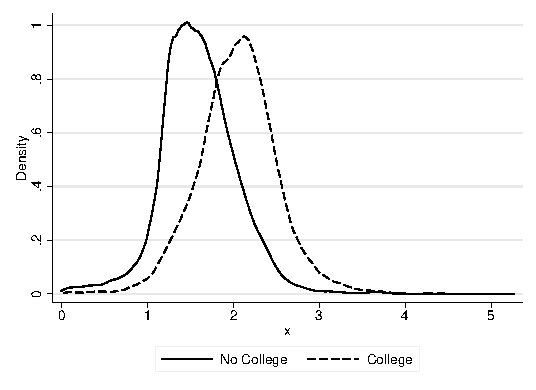
\includegraphics{logs/density.pdf}
\caption{Wage density}
\end{figure}

\begin{table}[ht]
\caption{Regression analysis}
\label{tab:stata}
  \begin{center}
\begin{tabular}{lccc}
\hline \noalign{\smallskip} & Simple model & Include capital & Full model\\
\noalign{\smallskip}\hline \noalign{\smallskip}Education & 0.3169*** & 0.212*** & 0.2***\\
 & \begin{footnotesize}(0.0093)\end{footnotesize} & \begin{footnotesize}(0.020)\end{footnotesize} & \begin{footnotesize}(0.0)\end{footnotesize}\\
\noalign{\smallskip}Capital &  & 0.125*** & 0.2***\\
 & \begin{footnotesize}\end{footnotesize} & \begin{footnotesize}(0.029)\end{footnotesize} & \begin{footnotesize}(0.0)\end{footnotesize}\\
\noalign{\smallskip}Openness degree &  &  & 0.0***\\
 & \begin{footnotesize}\end{footnotesize} & \begin{footnotesize}\end{footnotesize} & \begin{footnotesize}(0.0)\end{footnotesize}\\
\noalign{\smallskip}$R^2$ & 0.58 & 0.54 & 0.59\\
RMSE & 0.78 & 0.70 & 0.67\\
$N$ & 857 & 234 & 234\\
\noalign{\smallskip}\hline\end{tabular}\\
\smallskip\begin{footnotesize}\ * $p<0$.1; ** $p<0$.05; *** $p<0$.01\end{footnotesize}\\
\smallskip
\end{center}

\end{table}

\hypertarget{use-stata-to-export-statistics-to-excel}{%
\subsection{Use Stata to export statistics to Excel}\label{use-stata-to-export-statistics-to-excel}}

We now export a set of statistics to an Excel file.

\begin{verbatim}
version 16.1

c:\ado\plus/x/xtabond2.ado

Checksum for c:/ado/plus/x/xtabond2.ado = 3720163387, size = 40472

C:\Users\mangelo.EEG\Documents\GitHub\prjs\logs



Variable   Obs Unique      Mean       Min       Max  Label
-------------------------------------------------------------------------------
country    839    106         .         .         .  Country name
year       839      9  1980.906      1960      2000  Year of observation
education  839    574  4.794076       .04     12.25  Education
lngdp      839    838  9.308131  5.983335  12.51058  Log Real GDP per Worker
open       839      2  .4982122         0         1  1 = high degree of open...
gdp        839    838  20100.66  396.7612  271192.2  GDP level
-------------------------------------------------------------------------------


Note: file will be replaced when the first putexcel command is issued


`"a"' `"b"' `"c"' `"d"' `"e"' `"f"' `"g"' `"h"' `"i"' `"j"' `"k"' `"l"' `"m"' `
> "n"' `"p"' `"r"' `"s"' `"t"' `"u"' `"v"' `"z"'

  8.                         quietly {
  9.                                 collapse (mean) lngdp education,by(country
> )
 10.                                         putexcel set descriptives.xlsx, sh
> eet("FIRST LETTER `vv'") modify
 11.                                         
 19.                                                 putexcel D3 = matrix(t),nf
> ormat("0.00")
 20.                                 }
 21.                         }
 22.                         



Country's first letter:     a

    Number of countries:    .




Country's first letter:     b

    Number of countries:    .




Country's first letter:     c

    Number of countries:    .




Country's first letter:     d

    Number of countries:    .




Country's first letter:     e

    Number of countries:    .




Country's first letter:     f

    Number of countries:    .




Country's first letter:     g

    Number of countries:    .




Country's first letter:     h

    Number of countries:    .




Country's first letter:     i

    Number of countries:    .




Country's first letter:     j

    Number of countries:    .




Country's first letter:     k

    Number of countries:    .




Country's first letter:     l

    Number of countries:    .




Country's first letter:     m

    Number of countries:    .




Country's first letter:     n

    Number of countries:    .




Country's first letter:     p

    Number of countries:    .




Country's first letter:     r

    Number of countries:    .




Country's first letter:     s

    Number of countries:    .




Country's first letter:     t

    Number of countries:    .




Country's first letter:     u

    Number of countries:    .




Country's first letter:     v

    Number of countries:    .

insufficient observations
r(2001);

end of do-file
r(2001);
\end{verbatim}

See Figure \ref{fig:fig-tmp}.

\begin{figure}[ht]

{\centering \includegraphics{RMarkdown_Report_files/figure-latex/fig-tmp-1} 

}

\caption{Scatterplot test MP}\label{fig:fig-tmp}
\end{figure}

\hypertarget{final-remarks}{%
\section{Final remarks}\label{final-remarks}}

Check the replication package for Bonhomme, Lamadon and Manresa (2019): \url{https://github.com/tlamadon/blm-replicate}

\newpage

\hypertarget{references}{%
\section*{References}\label{references}}
\addcontentsline{toc}{section}{References}

\hypertarget{refs}{}
\begin{CSLReferences}{1}{0}
\leavevmode\hypertarget{ref-arellano2003panel}{}%
Arellano, Manuel. 2003. \emph{Panel Data Econometrics}. Oxford University Press.

\leavevmode\hypertarget{ref-arellano1991some}{}%
Arellano, Manuel and Stephen Bond. 1991. {``Some Tests of Specification for Panel Data: Monte Carlo Evidence and an Application to Employment Equations.''} \emph{The Review of Economic Studies} 58(2):277--97.

\leavevmode\hypertarget{ref-arellano1995another}{}%
Arellano, Manuel and Olympia Bover. 1995. {``Another Look at the Instrumental Variable Estimation of Error-Components Models.''} \emph{Journal of Econometrics} 68(1):29--51.

\leavevmode\hypertarget{ref-bb98}{}%
Blundell, Richard and Stephen Bond. 1998. {``Initial Conditions and Moment Restrictions in Dynamic Panel Data Models.''} \emph{Journal of Econometrics} 87(1):115--43.

\end{CSLReferences}

\hypertarget{appendix-chunk-options}{%
\section*{Appendix: Chunk options}\label{appendix-chunk-options}}
\addcontentsline{toc}{section}{Appendix: Chunk options}

\hypertarget{software-versioning}{%
\subsection{Software versioning}\label{software-versioning}}

\hypertarget{r-1}{%
\subsubsection{R}\label{r-1}}

\begin{Shaded}
\begin{Highlighting}[]
\FunctionTok{cat}\NormalTok{(}\FunctionTok{paste}\NormalTok{(}\StringTok{"\#"}\NormalTok{, }\FunctionTok{capture.output}\NormalTok{(}\FunctionTok{sessionInfo}\NormalTok{()), }\StringTok{"}\SpecialCharTok{\textbackslash{}n}\StringTok{"}\NormalTok{, }\AttributeTok{collapse =}\StringTok{""}\NormalTok{))}
\end{Highlighting}
\end{Shaded}

\begin{verbatim}
# R version 4.1.0 (2021-05-18) 
# Platform: x86_64-w64-mingw32/x64 (64-bit) 
# Running under: Windows 10 x64 (build 18363) 
#  
# Matrix products: default 
#  
# locale: 
# [1] LC_COLLATE=Portuguese_Portugal.1252  LC_CTYPE=C                           
# [3] LC_MONETARY=Portuguese_Portugal.1252 LC_NUMERIC=C                         
# [5] LC_TIME=Portuguese_Portugal.1252     
#  
# attached base packages: 
# [1] stats     graphics  grDevices utils     datasets  methods   base      
#  
# other attached packages: 
#  [1] plotly_4.9.4.1      naniar_0.6.1        visdat_0.5.3        
#  [4] dlookr_0.4.5        dplyr_1.0.6         ggplot2_3.3.3       
#  [7] haven_2.4.1         ExPanDaR_0.5.3      JuliaCall_0.17.4    
# [10] Statamarkdown_0.6.1 stargazer_5.2.2     reticulate_1.20     
#  
# loaded via a namespace (and not attached): 
#   [1] colorspace_2.0-1      ellipsis_0.3.2        class_7.3-19          
#   [4] rio_0.5.26            htmlTable_2.2.1       base64enc_0.1-3       
#   [7] rstudioapi_0.13       proxy_0.4-25          farver_2.1.0          
#  [10] DT_0.18               mvtnorm_1.1-1         fansi_0.4.2           
#  [13] xml2_1.3.2            splines_4.1.0         extrafont_0.17        
#  [16] libcoin_1.0-8         knitr_1.33            Formula_1.2-4         
#  [19] jsonlite_1.7.2        Rttf2pt1_1.3.8        cluster_2.1.2         
#  [22] png_0.1-7             shiny_1.6.0           readr_1.4.0           
#  [25] compiler_4.1.0        httr_1.4.2            tictoc_1.0.1          
#  [28] backports_1.2.1       lazyeval_0.2.2        assertthat_0.2.1      
#  [31] Matrix_1.3-3          fastmap_1.1.0         cli_2.5.0             
#  [34] later_1.2.0           hrbrthemes_0.8.0      htmltools_0.5.1.1     
#  [37] tools_4.1.0           partykit_1.2-13       gtable_0.3.0          
#  [40] glue_1.4.2            Rcpp_1.0.6            carData_3.0-4         
#  [43] cellranger_1.1.0      vctrs_0.3.8           svglite_2.0.0         
#  [46] extrafontdb_1.0       crosstalk_1.1.1       inum_1.0-4            
#  [49] xfun_0.23             stringr_1.4.0         openxlsx_4.2.3        
#  [52] rvest_1.0.0           mime_0.11             lifecycle_1.0.0       
#  [55] shinycssloaders_1.0.0 RcmdrMisc_2.7-1       MASS_7.3-54           
#  [58] zoo_1.8-9             scales_1.1.1          hms_1.1.0             
#  [61] promises_1.2.0.1      sandwich_3.0-1        RColorBrewer_1.1-2    
#  [64] yaml_2.2.1            curl_4.3.1            gridExtra_2.3         
#  [67] UpSetR_1.4.0          gdtools_0.2.3         rpart_4.1-15          
#  [70] latticeExtra_0.6-29   stringi_1.6.2         highr_0.9             
#  [73] corrplot_0.88         nortest_1.0-4         e1071_1.7-7           
#  [76] checkmate_2.0.0       zip_2.1.1             rlang_0.4.11          
#  [79] pkgconfig_2.0.3       systemfonts_1.0.2     evaluate_0.14         
#  [82] lattice_0.20-44       purrr_0.3.4           labeling_0.4.2        
#  [85] htmlwidgets_1.5.3     tidyselect_1.1.1      plyr_1.8.6            
#  [88] magrittr_2.0.1        bookdown_0.22         R6_2.5.0              
#  [91] generics_0.1.0        Hmisc_4.5-0           DBI_1.1.1             
#  [94] pillar_1.6.1          foreign_0.8-81        withr_2.4.2           
#  [97] prettydoc_0.4.1       survival_3.2-11       abind_1.4-5           
# [100] nnet_7.3-16           tibble_3.1.2          crayon_1.4.1          
# [103] car_3.0-10            utf8_1.2.1            rmarkdown_2.8         
# [106] jpeg_0.1-8.1          grid_4.1.0            readxl_1.3.1          
# [109] data.table_1.14.0     forcats_0.5.1         webshot_0.5.2         
# [112] digest_0.6.27         xtable_1.8-4          tidyr_1.1.3           
# [115] httpuv_1.6.1          openssl_1.4.4         munsell_0.5.0         
# [118] viridisLite_0.4.0     kableExtra_1.3.4      askpass_1.1           
\end{verbatim}

\begin{Shaded}
\begin{Highlighting}[]
  \CommentTok{\# or use message() instead of cat()}
\end{Highlighting}
\end{Shaded}

\hypertarget{python-1}{%
\subsubsection{Python}\label{python-1}}

\begin{Shaded}
\begin{Highlighting}[]
\ImportTok{import}\NormalTok{ sys}
\BuiltInTok{print}\NormalTok{(sys.version)}
\end{Highlighting}
\end{Shaded}

\begin{verbatim}
3.9.4 (tags/v3.9.4:1f2e308, Apr  6 2021, 13:40:21) [MSC v.1928 64 bit (AMD64)]
\end{verbatim}

\hypertarget{julia}{%
\subsubsection{Julia}\label{julia}}

\begin{verbatim}
v"1.6.1"
\end{verbatim}

\hypertarget{stata}{%
\subsubsection{Stata}\label{stata}}

\begin{verbatim}
version 16.1

c:\ado\plus/x/xtabond2.ado

Checksum for c:/ado/plus/x/xtabond2.ado = 3720163387, size = 40472
\end{verbatim}

\hypertarget{all-the-code-in-the-paper}{%
\subsection{All the code in the paper}\label{all-the-code-in-the-paper}}

To simply attach all the code you used in the PDF file in the appendix see the R chunk in the underlying \texttt{.rmd} file:

\begin{Shaded}
\begin{Highlighting}[]
\NormalTok{knitr}\SpecialCharTok{::}\NormalTok{opts\_chunk}\SpecialCharTok{$}\FunctionTok{set}\NormalTok{(}\AttributeTok{cache =} \ConstantTok{FALSE}\NormalTok{)}
\CommentTok{\# Use chache = TRUE if you want to speed up compilation}

\CommentTok{\# A function to allow for showing some of the inline code}
\NormalTok{rinline }\OtherTok{\textless{}{-}} \ControlFlowTok{function}\NormalTok{(code)\{}
\NormalTok{  html }\OtherTok{\textless{}{-}} \StringTok{\textquotesingle{}\textless{}code  class="r"\textgreater{}\textasciigrave{}\textasciigrave{}\textasciigrave{} \textasciigrave{}r CODE\textasciigrave{} \textasciigrave{}\textasciigrave{}\textasciigrave{}\textless{}/code\textgreater{}\textquotesingle{}}
  \FunctionTok{sub}\NormalTok{(}\StringTok{"CODE"}\NormalTok{, code, html)}

  \DocumentationTok{\#\#https://opensource.com/article/19/5/python{-}3{-}default{-}mac}

  \FunctionTok{Sys.setenv}\NormalTok{(}\AttributeTok{RETICULATE\_PYTHON =} \StringTok{"C:/Users/mangelo.EEG/AppData/Local/Microsoft/WindowsApps/python3"}\NormalTok{)}

\DocumentationTok{\#\#install.packages("reticulate")}
\FunctionTok{library}\NormalTok{(reticulate)}
\DocumentationTok{\#\#use\_python("/Library/Frameworks/Python.framework/Versions/3.8/bin/python3")}

\FunctionTok{use\_virtualenv}\NormalTok{(}\StringTok{"C:/Users/mangelo.EEG/Documents/python"}\NormalTok{)}

\DocumentationTok{\#\#knitr::opts\_chunk$set(python.reticulate=FALSE)}

\CommentTok{\# library(devtools) \# before this you may need to install devtools}
\CommentTok{\# install\_github("hemken/Statamarkdown")}

\FunctionTok{library}\NormalTok{(JuliaCall)}

\FunctionTok{library}\NormalTok{(Statamarkdown)}
\NormalTok{stataexe }\OtherTok{\textless{}{-}} \StringTok{"C:/Program Files/Stata16/StataMP{-}64.exe"}
\NormalTok{knitr}\SpecialCharTok{::}\NormalTok{opts\_chunk}\SpecialCharTok{$}\FunctionTok{set}\NormalTok{(}\AttributeTok{engine.path=}\FunctionTok{list}\NormalTok{(}\AttributeTok{stata=}\NormalTok{stataexe))}

\NormalTok{\}}
\FunctionTok{Sys.setenv}\NormalTok{(}\AttributeTok{RETICULATE\_PYTHON =} \StringTok{"C:/Program Files/Python39/python.exe"}\NormalTok{)}
\FunctionTok{library}\NormalTok{(reticulate)}
\FunctionTok{use\_virtualenv}\NormalTok{(}\StringTok{"C:/Users/mangelo.EEG/Documents/python"}\NormalTok{)}
\FunctionTok{library}\NormalTok{(stargazer)}
\FunctionTok{library}\NormalTok{(Statamarkdown)}
\NormalTok{stataexe }\OtherTok{\textless{}{-}} \StringTok{"C:/Program Files/Stata16/StataMP{-}64.exe"}
\CommentTok{\#stataexe \textless{}{-} "/Applications/Stata15/StataMP.app/Contents/MacOS//stata{-}mp"}
\NormalTok{knitr}\SpecialCharTok{::}\NormalTok{opts\_chunk}\SpecialCharTok{$}\FunctionTok{set}\NormalTok{(}\AttributeTok{engine.path=}\FunctionTok{list}\NormalTok{(}\AttributeTok{stata=}\NormalTok{stataexe))}
\FunctionTok{library}\NormalTok{(JuliaCall)}
\FunctionTok{options}\NormalTok{(}\AttributeTok{JULIA\_HOME =} \StringTok{"C:/Users/mangelo.EEG/AppData/Local/Programs/Julia{-}1.6.1/bin"}\NormalTok{)}
\FunctionTok{julia\_setup}\NormalTok{()}

\DocumentationTok{\#\# ExPanDaR: Explore Panel Data Interactively}

  \FunctionTok{library}\NormalTok{(ExPanDaR)}

    \DocumentationTok{\#\# type ExPanD() in the Console}

\FunctionTok{setwd}\NormalTok{(}\StringTok{"C:/Users/mangelo.EEG/Documents/GitHub/prjs/logs"}\NormalTok{)}

\FunctionTok{library}\NormalTok{(haven)}
\FunctionTok{library}\NormalTok{(ggplot2)}

\NormalTok{nlswork }\OtherTok{\textless{}{-}} \FunctionTok{read\_dta}\NormalTok{(}\StringTok{"C:/Users/mangelo.EEG/Documents/GitHub/prjs/data/nlswork.dta"}\NormalTok{)}

\NormalTok{nls}\OtherTok{\textless{}{-}}\FunctionTok{data.frame}\NormalTok{(nlswork)}

\FunctionTok{attach}\NormalTok{(nlswork)}

\FunctionTok{head}\NormalTok{(nlswork)}

\FunctionTok{library}\NormalTok{(stargazer)}
\FunctionTok{stargazer}\NormalTok{(nls,}
          \AttributeTok{title =} \StringTok{"Summary statistics"}\NormalTok{,}
          \AttributeTok{label=}\StringTok{"tab1"}\NormalTok{,}
          \AttributeTok{table.placement =} \StringTok{"ht"}\NormalTok{,}
          \AttributeTok{header=}\ConstantTok{FALSE}\NormalTok{)}

\FunctionTok{library}\NormalTok{(dplyr)}
\FunctionTok{library}\NormalTok{(dlookr)}
\FunctionTok{library}\NormalTok{(ggplot2)}

\DocumentationTok{\#\#eda\_report(nlswork,output\_dir = "C:/Users/mangelo.EEG/Documents/GitHub/prjs/reports/",output\_file = "eda\_report.pdf")}

\DocumentationTok{\#\# The data}

\FunctionTok{names}\NormalTok{(nlswork)}
\DocumentationTok{\#\#summary(nlswork)}

\DocumentationTok{\#\# Missing values}

\FunctionTok{library}\NormalTok{(}\StringTok{"visdat"}\NormalTok{)}

  \FunctionTok{vis\_dat}\NormalTok{(nlswork)}

\DocumentationTok{\#\# https://cran.r{-}project.org/web/packages/naniar/vignettes/naniar{-}visualisation.html}

\FunctionTok{library}\NormalTok{(naniar)}

  \FunctionTok{vis\_miss}\NormalTok{(nlswork)}

  \FunctionTok{gg\_miss\_upset}\NormalTok{(nlswork)}

\DocumentationTok{\#\# GRAPHS}
\NormalTok{dplyr}\SpecialCharTok{::}\FunctionTok{glimpse}\NormalTok{(nlswork}\SpecialCharTok{$}\NormalTok{ln\_wage)}
\NormalTok{d }\OtherTok{\textless{}{-}} \FunctionTok{density}\NormalTok{(ln\_wage)}
\FunctionTok{plot}\NormalTok{(d)}

\FunctionTok{plot}\NormalTok{(nls}\SpecialCharTok{$}\NormalTok{ln\_wage,nls}\SpecialCharTok{$}\NormalTok{ttl\_exp)}

\FunctionTok{ggplot}\NormalTok{(nlswork,}
       \FunctionTok{aes}\NormalTok{(}\AttributeTok{x =}\NormalTok{ hours,}
           \AttributeTok{y =}\NormalTok{ year)) }\SpecialCharTok{+}
\FunctionTok{geom\_miss\_point}\NormalTok{()}

\FunctionTok{ggplot}\NormalTok{(nlswork,}
       \FunctionTok{aes}\NormalTok{(}\AttributeTok{x =}\NormalTok{ hours,}
           \AttributeTok{y =}\NormalTok{ year)) }\SpecialCharTok{+}
\FunctionTok{geom\_miss\_point}\NormalTok{() }\SpecialCharTok{+}
\FunctionTok{facet\_wrap}\NormalTok{(race)}

\NormalTok{stats }\OtherTok{\textless{}{-}} \FunctionTok{summary}\NormalTok{(nlswork}\SpecialCharTok{$}\NormalTok{age)}

\FunctionTok{library}\NormalTok{(stargazer)}
\FunctionTok{stargazer}\NormalTok{(cars,}
          \AttributeTok{title =} \StringTok{"Summary table with stargazer"}\NormalTok{,}
          \AttributeTok{label=}\StringTok{"tab1cars"}\NormalTok{,}
          \AttributeTok{table.placement =} \StringTok{"H"}\NormalTok{,}
          \AttributeTok{header=}\ConstantTok{FALSE}\NormalTok{)}
\FunctionTok{library}\NormalTok{(stargazer)}
\NormalTok{model1 }\OtherTok{\textless{}{-}} \FunctionTok{lm}\NormalTok{(speed }\SpecialCharTok{\textasciitilde{}}\NormalTok{ dist, }\AttributeTok{data =}\NormalTok{ cars)}
\NormalTok{model2 }\OtherTok{\textless{}{-}} \FunctionTok{lm}\NormalTok{(speed }\SpecialCharTok{\textasciitilde{}}\NormalTok{ dist, }\AttributeTok{data =}\NormalTok{ cars)}
\NormalTok{model3 }\OtherTok{\textless{}{-}} \FunctionTok{lm}\NormalTok{(dist }\SpecialCharTok{\textasciitilde{}}\NormalTok{ speed, }\AttributeTok{data =}\NormalTok{ cars)}
\FunctionTok{stargazer}\NormalTok{(model1, model2, model3,}
          \AttributeTok{title =} \StringTok{"Regression table with stargazer"}\NormalTok{,}
          \AttributeTok{label=}\StringTok{"tab2"}\NormalTok{,}
          \AttributeTok{table.placement =} \StringTok{"H"}\NormalTok{,}
          \AttributeTok{column.labels =} \FunctionTok{c}\NormalTok{(}\StringTok{"M1"}\NormalTok{, }\StringTok{"M2"}\NormalTok{, }\StringTok{"M3"}\NormalTok{),}
          \AttributeTok{model.numbers =} \ConstantTok{FALSE}\NormalTok{,}
          \AttributeTok{header=}\ConstantTok{FALSE}\NormalTok{)}
\FunctionTok{plot}\NormalTok{(cars}\SpecialCharTok{$}\NormalTok{speed, cars}\SpecialCharTok{$}\NormalTok{dist)}
\NormalTok{mtcars}\SpecialCharTok{$}\NormalTok{cyl }\OtherTok{\textless{}{-}} \FunctionTok{as.factor}\NormalTok{(mtcars}\SpecialCharTok{$}\NormalTok{cyl) }\CommentTok{\# Convert cyl to factor}
\FunctionTok{library}\NormalTok{(ggplot2)}
\FunctionTok{ggplot}\NormalTok{(mtcars, }\FunctionTok{aes}\NormalTok{(}\AttributeTok{x=}\NormalTok{wt, }\AttributeTok{y=}\NormalTok{mpg, }\AttributeTok{shape=}\NormalTok{cyl)) }\SpecialCharTok{+} \FunctionTok{geom\_point}\NormalTok{() }\SpecialCharTok{+}
  \FunctionTok{labs}\NormalTok{(}\AttributeTok{x=}\StringTok{"Weight (lb/1000)"}\NormalTok{, }\AttributeTok{y =} \StringTok{"Miles/(US) gallon"}\NormalTok{,}
       \AttributeTok{shape=}\StringTok{"Number of }\SpecialCharTok{\textbackslash{}n}\StringTok{ Cylinders"}\NormalTok{) }\SpecialCharTok{+} \FunctionTok{theme\_classic}\NormalTok{()}
\FunctionTok{library}\NormalTok{(plotly)}
\NormalTok{p }\OtherTok{\textless{}{-}} \FunctionTok{plot\_ly}\NormalTok{(cars, }\AttributeTok{type =} \StringTok{"scatter"}\NormalTok{, }\AttributeTok{mode=}\StringTok{"markers"}\NormalTok{,}
        \AttributeTok{x=}\SpecialCharTok{\textasciitilde{}}\NormalTok{speed,}
        \AttributeTok{y=}\SpecialCharTok{\textasciitilde{}}\NormalTok{dist)}
\CommentTok{\#Sys.setenv(\textquotesingle{}MAPBOX\_TOKEN\textquotesingle{} = \textquotesingle{}12423423\textquotesingle{}) \# set arbitrary token}
\CommentTok{\#orca(p, "logs/plotly{-}plot.pdf")}
\NormalTok{import sys}
\FunctionTok{print}\NormalTok{(sys.version)}


\NormalTok{import json}
\DocumentationTok{\#\#from json.decoder import JSONDecodeError}
\NormalTok{import requests}
\NormalTok{import numpy as np}
\NormalTok{import pandas as pd}

\DocumentationTok{\#\# INE: https://www.ine.pt/ine/json\_indicador/pindica.jsp?}
\DocumentationTok{\#\# op=2\&varcd=0008074\&Dim1=S7A2015\&Dim2=200\&Dim3=3\&lang=PT}

\CommentTok{\# api{-}endpoint}

\NormalTok{URL }\OtherTok{=} \StringTok{"https://www.ine.pt/ine/json\_indicador/pindica.jsp"}

\CommentTok{\# define parameters}

\NormalTok{OP}\OtherTok{=}\StringTok{"2"}
\NormalTok{VARCD}\OtherTok{=}\StringTok{"0008074"}
\NormalTok{DIM1}\OtherTok{=}\StringTok{"S7A2015"}
\NormalTok{DIM2}\OtherTok{=}\StringTok{"200"}
\NormalTok{DIM3}\OtherTok{=}\StringTok{"3"}
\NormalTok{LANG}\OtherTok{=}\StringTok{"PT"}


\CommentTok{\# defining a params dict for the parameters to be sent to the API}
\NormalTok{PARAMS }\OtherTok{=}\NormalTok{ \{}\StringTok{\textquotesingle{}op\textquotesingle{}}\SpecialCharTok{:}\NormalTok{OP,}\StringTok{\textquotesingle{}varcd\textquotesingle{}}\SpecialCharTok{:}\NormalTok{VARCD,}\StringTok{\textquotesingle{}Dim1\textquotesingle{}}\SpecialCharTok{:}\NormalTok{DIM1,}\StringTok{\textquotesingle{}Dim2\textquotesingle{}}\SpecialCharTok{:}\NormalTok{DIM2,}\StringTok{\textquotesingle{}Dim3\textquotesingle{}}\SpecialCharTok{:}\NormalTok{DIM3,}\StringTok{\textquotesingle{}lang\textquotesingle{}}\SpecialCharTok{:}\NormalTok{LANG\}}

\CommentTok{\# sending get request and saving the response as response object}
\NormalTok{r }\OtherTok{=} \FunctionTok{requests.get}\NormalTok{(}\AttributeTok{url =}\NormalTok{ URL,}\AttributeTok{params=}\NormalTok{PARAMS)}

\CommentTok{\# extracting data in json format}
\NormalTok{data }\OtherTok{=} \FunctionTok{r.json}\NormalTok{()}

\NormalTok{valor }\OtherTok{=}\NormalTok{ data[}\DecValTok{0}\NormalTok{][}\StringTok{\textquotesingle{}Dados\textquotesingle{}}\NormalTok{][}\StringTok{\textquotesingle{}2015\textquotesingle{}}\NormalTok{][}\DecValTok{0}\NormalTok{][}\StringTok{\textquotesingle{}valor\textquotesingle{}}\NormalTok{]}

\NormalTok{valor}

\NormalTok{  cd C}\SpecialCharTok{:}\ErrorTok{/}\NormalTok{Users}\SpecialCharTok{/}\NormalTok{mangelo.EEG}\SpecialCharTok{/}\NormalTok{Documents}\SpecialCharTok{/}\NormalTok{GitHub}\SpecialCharTok{/}\NormalTok{prjs}\SpecialCharTok{/}\NormalTok{pdfs}
\NormalTok{    find . }\SpecialCharTok{{-}}\NormalTok{name }\StringTok{\textquotesingle{}*.pdf\textquotesingle{}} \SpecialCharTok{{-}}\NormalTok{print0 }\SpecialCharTok{|}\NormalTok{ xargs }\SpecialCharTok{{-}}\DecValTok{0} \SpecialCharTok{{-}}\NormalTok{n1 pdfsandwich }\SpecialCharTok{{-}}\NormalTok{gray}
\NormalTok{    find . }\SpecialCharTok{{-}}\NormalTok{name }\StringTok{\textquotesingle{}*ocr.pdf\textquotesingle{}} \SpecialCharTok{{-}}\NormalTok{print0 }\SpecialCharTok{|}\NormalTok{ xargs }\SpecialCharTok{{-}}\DecValTok{0} \SpecialCharTok{{-}}\NormalTok{n1 pdftotext}
\NormalTok{import os}
\NormalTok{import numpy as np}
\NormalTok{import pandas as pd}
\NormalTok{import re}

\DocumentationTok{\#\# CHECK PyPDF2}

\DocumentationTok{\#\# wget {-}A pdf {-}m {-}p {-}E {-}k {-}K {-}np https://joram.madeira.gov.pt/joram/4serie/}
\DocumentationTok{\#\# find . {-}name \textquotesingle{}*.pdf\textquotesingle{} {-}print0 | xargs {-}0 {-}n1 pdfsandwich {-}gray}
\DocumentationTok{\#\# find . {-}name \textquotesingle{}*ocr.pdf\textquotesingle{} {-}print0 | xargs {-}0 {-}n1 pdftotext}

\CommentTok{\# Create list with .txt files for the specified folder}
\NormalTok{files\_list }\OtherTok{=} \FunctionTok{list}\NormalTok{()}
\ControlFlowTok{for}\NormalTok{ (dirpath, dirnames, filenames) }\ControlFlowTok{in} \FunctionTok{os.walk}\NormalTok{(}\StringTok{\textquotesingle{}C:/Users/mangelo.EEG/Documents/GitHub/prjs/pdfs/\textquotesingle{}}\NormalTok{)}\SpecialCharTok{:}
\NormalTok{    files\_list }\SpecialCharTok{+}\ErrorTok{=}\NormalTok{ [}\FunctionTok{os.path.join}\NormalTok{(dirpath, file)}
                   \ControlFlowTok{for}\NormalTok{ file }\ControlFlowTok{in}\NormalTok{ filenames }\ControlFlowTok{if} \FunctionTok{file.endswith}\NormalTok{(}\StringTok{\textquotesingle{}.txt\textquotesingle{}}\NormalTok{)]}


\DocumentationTok{\#\#print("START:FILES {-}{-} list")}

\DocumentationTok{\#\#print(files\_list)}

\DocumentationTok{\#\#print("}\RegionMarkerTok{END}\DocumentationTok{:FILES {-}{-} list")}

\NormalTok{p1 }\OtherTok{=}\NormalTok{ r}\StringTok{\textquotesingle{}PORTARIA\textquotesingle{}}
\NormalTok{p2 }\OtherTok{=}\NormalTok{ r}\StringTok{\textquotesingle{}EXTENSAO\textquotesingle{}}
\NormalTok{p3 }\OtherTok{=}\NormalTok{ r}\StringTok{\textquotesingle{}Materiais\textquotesingle{}}
\NormalTok{p5 }\OtherTok{=}\NormalTok{ r}\StringTok{\textquotesingle{}PE das\textquotesingle{}}

\NormalTok{linha }\OtherTok{=}\NormalTok{ []}
\NormalTok{output }\OtherTok{=}\NormalTok{ []}
\NormalTok{other }\OtherTok{=}\NormalTok{ []}
\NormalTok{palavra }\OtherTok{=}\NormalTok{ []}
\NormalTok{source }\OtherTok{=}\NormalTok{ []}

\ControlFlowTok{for}\NormalTok{ file }\ControlFlowTok{in}\NormalTok{ files\_list}\SpecialCharTok{:}

\NormalTok{    f }\OtherTok{=} \FunctionTok{open}\NormalTok{(file, }\StringTok{"r"}\NormalTok{, }\AttributeTok{encoding=}\StringTok{\textquotesingle{}latin8\textquotesingle{}}\NormalTok{)}
\NormalTok{    data }\OtherTok{=} \FunctionTok{f.read}\NormalTok{()}
    \FunctionTok{f.close}\NormalTok{()}

\NormalTok{    line }\OtherTok{=}\NormalTok{ []}
\NormalTok{    nh }\OtherTok{=} \DecValTok{0}

\NormalTok{    tmp1 }\OtherTok{=} \FunctionTok{str}\NormalTok{(data)}
    \CommentTok{\#print(tmp1)}
\NormalTok{    tmp2 }\OtherTok{=} \FunctionTok{tmp1.splitlines}\NormalTok{()}
    \CommentTok{\#print(tmp2)}
    \ControlFlowTok{for}\NormalTok{ n,tmp3 }\ControlFlowTok{in} \FunctionTok{enumerate}\NormalTok{(tmp2)}\SpecialCharTok{:}
        \CommentTok{\#print(tmp3)}
        \ControlFlowTok{if}\NormalTok{ (}\FunctionTok{tmp3.find}\NormalTok{(}\StringTok{"PE das"}\NormalTok{) }\SpecialCharTok{==} \DecValTok{0}\NormalTok{)}\SpecialCharTok{:}
\NormalTok{            tmp4 }\OtherTok{=}\NormalTok{ tmp3 }\SpecialCharTok{+}\NormalTok{ tmp2[}\DecValTok{2}\NormalTok{]}
            \FunctionTok{line.append}\NormalTok{(tmp4)}
            \CommentTok{\#print(n)}
\NormalTok{            nh }\OtherTok{=} \DecValTok{1}
        \FunctionTok{elif}\NormalTok{ (nh }\SpecialCharTok{==} \DecValTok{1}\NormalTok{)}\SpecialCharTok{:}
\NormalTok{            nh }\OtherTok{=} \DecValTok{0}
\NormalTok{            continue}
        \FunctionTok{elif}\NormalTok{ (nh }\SpecialCharTok{==} \DecValTok{0}\NormalTok{)}\SpecialCharTok{:}
            \FunctionTok{line.append}\NormalTok{(tmp3)}

    \FunctionTok{print}\NormalTok{(line)}

    \FunctionTok{print}\NormalTok{(}\StringTok{"   "}\NormalTok{)}

    \FunctionTok{print}\NormalTok{(}\StringTok{"FILE: "}\NormalTok{, file[}\DecValTok{46}\SpecialCharTok{:{-}}\DecValTok{4}\NormalTok{])}

    \ControlFlowTok{for}\NormalTok{ num, word }\ControlFlowTok{in} \FunctionTok{enumerate}\NormalTok{(line)}\SpecialCharTok{:}
            \ControlFlowTok{if}\NormalTok{ num }\SpecialCharTok{==} \DecValTok{0}\SpecialCharTok{:}
\NormalTok{                continue}
            \ControlFlowTok{else}\SpecialCharTok{:}
\NormalTok{                match1 }\OtherTok{=} \FunctionTok{re.search}\NormalTok{(p1, word)}
\NormalTok{                match2 }\OtherTok{=} \FunctionTok{re.search}\NormalTok{(p2, word)}
\NormalTok{                match3 }\OtherTok{=} \FunctionTok{re.search}\NormalTok{(p3, word)}
\NormalTok{                match4 }\OtherTok{=} \FunctionTok{re.search}\NormalTok{(r}\StringTok{\textquotesingle{}\textbackslash{}d\{9\}\textquotesingle{}}\NormalTok{, word)}
\NormalTok{                match5 }\OtherTok{=} \FunctionTok{re.search}\NormalTok{(p5, word)}
                \DocumentationTok{\#\#print("   ")}
                \DocumentationTok{\#\#print("START: ",num)}

                \ControlFlowTok{if}\NormalTok{ match1}\SpecialCharTok{:}
                        \DocumentationTok{\#\#print("   ")}
                        \FunctionTok{print}\NormalTok{(}\StringTok{"match 1"}\NormalTok{)}
                        \ControlFlowTok{if}\NormalTok{ match4}\SpecialCharTok{:}
                            \DocumentationTok{\#\#print("   ")}
                            \FunctionTok{print}\NormalTok{(}\StringTok{"match 4"}\NormalTok{)}
                            \FunctionTok{linha.append}\NormalTok{(num)}
                            \FunctionTok{output.append}\NormalTok{(}\FunctionTok{re.search}\NormalTok{(r}\StringTok{\textquotesingle{}\textbackslash{}d\{9\}\textquotesingle{}}\NormalTok{, word)}\FunctionTok{.group}\NormalTok{())}
                            \FunctionTok{other.append}\NormalTok{(}\StringTok{"vazio"}\NormalTok{)}
                            \FunctionTok{palavra.append}\NormalTok{(p1)}
                            \FunctionTok{source.append}\NormalTok{(file[}\DecValTok{46}\SpecialCharTok{:{-}}\DecValTok{4}\NormalTok{])}
\NormalTok{                elif match2}\SpecialCharTok{:}
                            \DocumentationTok{\#\#print("   ")}
                            \FunctionTok{print}\NormalTok{(}\StringTok{"match 2"}\NormalTok{)}
                            \FunctionTok{linha.append}\NormalTok{(num)}
                            \FunctionTok{output.append}\NormalTok{(}\FunctionTok{re.search}\NormalTok{(r}\StringTok{\textquotesingle{}\textbackslash{}d\{9\}\textquotesingle{}}\NormalTok{, word)}\FunctionTok{.group}\NormalTok{())}
                            \FunctionTok{other.append}\NormalTok{(}\StringTok{"vazio"}\NormalTok{)}
                            \FunctionTok{palavra.append}\NormalTok{(p2)}
                            \FunctionTok{source.append}\NormalTok{(file[}\DecValTok{46}\SpecialCharTok{:{-}}\DecValTok{4}\NormalTok{])}
\NormalTok{                elif match3}\SpecialCharTok{:}
                            \DocumentationTok{\#\#print("   ")}
                            \FunctionTok{print}\NormalTok{(}\StringTok{"match 3"}\NormalTok{)}
                            \FunctionTok{linha.append}\NormalTok{(num)}
                            \FunctionTok{output.append}\NormalTok{(}\FunctionTok{re.search}\NormalTok{(r}\StringTok{\textquotesingle{}\textbackslash{}d\{9\}\textquotesingle{}}\NormalTok{, word)}\FunctionTok{.group}\NormalTok{())}
                            \FunctionTok{other.append}\NormalTok{(}\StringTok{"vazio"}\NormalTok{)}
                            \FunctionTok{palavra.append}\NormalTok{(p3)}
                            \FunctionTok{source.append}\NormalTok{(file[}\DecValTok{46}\SpecialCharTok{:{-}}\DecValTok{4}\NormalTok{])}
\NormalTok{                elif match5}\SpecialCharTok{:}
                            \DocumentationTok{\#\#print("   ")}
                            \FunctionTok{print}\NormalTok{(}\StringTok{"{-}\textgreater{} match 5"}\NormalTok{)}
                            \DocumentationTok{\#\#word.sub(" e o ", " e a ",1)}
                            \FunctionTok{print}\NormalTok{(word)}
                            \FunctionTok{linha.append}\NormalTok{(num)}

                            \ControlFlowTok{if}\NormalTok{ (}\FunctionTok{word.find}\NormalTok{(}\StringTok{" e o "}\NormalTok{) }\SpecialCharTok{\textgreater{}} \DecValTok{0}\NormalTok{)}\SpecialCharTok{:}
                                \FunctionTok{print}\NormalTok{(}\StringTok{"11111"}\NormalTok{)}
                                \FunctionTok{output.append}\NormalTok{((}\FunctionTok{word.split}\NormalTok{(}\StringTok{"re a"}\NormalTok{, }\DecValTok{1}\NormalTok{)[}\DecValTok{1}\NormalTok{])}\FunctionTok{.split}\NormalTok{(}\StringTok{" e o "}\NormalTok{, }\SpecialCharTok{{-}}\DecValTok{1}\NormalTok{)[}\SpecialCharTok{{-}}\DecValTok{2}\NormalTok{])}
                                \FunctionTok{other.append}\NormalTok{((}\FunctionTok{word.split}\NormalTok{(}\StringTok{"re a"}\NormalTok{, }\DecValTok{1}\NormalTok{)[}\DecValTok{1}\NormalTok{])}\FunctionTok{.split}\NormalTok{(}\StringTok{" e o "}\NormalTok{, }\DecValTok{1}\NormalTok{)[}\DecValTok{1}\NormalTok{])}
                            \FunctionTok{elif}\NormalTok{ (}\FunctionTok{word.find}\NormalTok{(}\StringTok{" e a "}\NormalTok{) }\SpecialCharTok{\textgreater{}} \DecValTok{0}\NormalTok{)}\SpecialCharTok{:}
                                \FunctionTok{print}\NormalTok{(}\StringTok{"99999"}\NormalTok{)}
                                \FunctionTok{output.append}\NormalTok{((}\FunctionTok{word.split}\NormalTok{(}\StringTok{"re a"}\NormalTok{, }\DecValTok{1}\NormalTok{)[}\DecValTok{1}\NormalTok{])}\FunctionTok{.split}\NormalTok{(}\StringTok{" e a "}\NormalTok{, }\SpecialCharTok{{-}}\DecValTok{1}\NormalTok{)[}\SpecialCharTok{{-}}\DecValTok{2}\NormalTok{])}
                                \FunctionTok{other.append}\NormalTok{((}\FunctionTok{word.split}\NormalTok{(}\StringTok{"re a"}\NormalTok{, }\DecValTok{1}\NormalTok{)[}\DecValTok{1}\NormalTok{])}\FunctionTok{.split}\NormalTok{(}\StringTok{" e a "}\NormalTok{, }\DecValTok{1}\NormalTok{)[}\DecValTok{1}\NormalTok{])}

                            \FunctionTok{palavra.append}\NormalTok{(p5)}
                            \FunctionTok{source.append}\NormalTok{(file[}\DecValTok{46}\SpecialCharTok{:{-}}\DecValTok{4}\NormalTok{])}
\DocumentationTok{\#\# o paragrafo tem de estar na mesma linha e temos de ter \textquotesingle{}e a\textquotesingle{} em vez de \textquotesingle{}e o\textquotesingle{}}
\NormalTok{df }\OtherTok{=} \FunctionTok{pd.DataFrame}\NormalTok{(\{}\StringTok{\textquotesingle{}linha\textquotesingle{}}\SpecialCharTok{:}\NormalTok{ linha, }\StringTok{\textquotesingle{}output\textquotesingle{}}\SpecialCharTok{:}\NormalTok{ output,}
                   \StringTok{\textquotesingle{}outra\textquotesingle{}}\SpecialCharTok{:}\NormalTok{ other, }\StringTok{\textquotesingle{}source\textquotesingle{}}\SpecialCharTok{:}\NormalTok{ source\})}
\FunctionTok{print}\NormalTok{(df)}

\FunctionTok{df.to\_csv}\NormalTok{(}\StringTok{\textquotesingle{}data/PE.csv\textquotesingle{}}\NormalTok{, }\AttributeTok{index=}\NormalTok{False)}
\FunctionTok{df.to\_stata}\NormalTok{(}\StringTok{\textquotesingle{}data/PE.dta\textquotesingle{}}\NormalTok{, }\AttributeTok{write\_index =}\NormalTok{ False)}


\NormalTok{quiet cd }\StringTok{"C:/Users/mangelo.EEG/Documents/GitHub/prjs/logs"}
\NormalTok{quiet import delimited }\StringTok{"C:/Users/mangelo.EEG/Documents/GitHub/prjs/data/PE.csv"}\NormalTok{, }\FunctionTok{encoding}\NormalTok{(ISO}\DecValTok{{-}8859{-}2}\NormalTok{) clear}
\NormalTok{tab source}

\NormalTok{python3 }\StringTok{"C:/Users/mangelo.EEG/Documents/GitHub/prjs/chunks/python\_chunk.py"}

\NormalTok{quietly\{}
\NormalTok{cd C}\SpecialCharTok{:}\ErrorTok{/}\NormalTok{Users}\SpecialCharTok{/}\NormalTok{mangelo.EEG}\SpecialCharTok{/}\NormalTok{Documents}\SpecialCharTok{/}\NormalTok{GitHub}\SpecialCharTok{/}\NormalTok{prjs}\SpecialCharTok{/}\NormalTok{chunks}

\NormalTok{use C}\SpecialCharTok{:}\ErrorTok{/}\NormalTok{Users}\SpecialCharTok{/}\NormalTok{mangelo.EEG}\SpecialCharTok{/}\NormalTok{Documents}\SpecialCharTok{/}\NormalTok{GitHub}\SpecialCharTok{/}\NormalTok{prjs}\SpecialCharTok{/}\NormalTok{data}\SpecialCharTok{/}\NormalTok{nipcs, clear}
\NormalTok{compress}
\NormalTok{contract nipc}
\NormalTok{drop \_freq}
\NormalTok{drop }\ControlFlowTok{if}\NormalTok{ nipc }\SpecialCharTok{==}\NormalTok{ .}
\NormalTok{format \%}\FloatTok{12.0}\NormalTok{f nipc}
\NormalTok{\}}

\SpecialCharTok{/}\ErrorTok{/}\NormalTok{codebook nipc}

\NormalTok{tab nipc}
\DocumentationTok{\#\# This is a julia language chunk.}
\DocumentationTok{\#\# In julia, the command without ending semicolon will trigger the display}
\DocumentationTok{\#\# so is JuliaCall package.}
\DocumentationTok{\#\# The julia display will follow immediately after the corresponding command}
\DocumentationTok{\#\# just as the R code in R Markdown.}

\NormalTok{using ReadStat}
\NormalTok{using StatFiles}
\NormalTok{using StatsBase}
\NormalTok{using DataFrames}
\NormalTok{using FixedEffectModels}

\SpecialCharTok{@}\NormalTok{time results\_hdfe1 }\OtherTok{=} \FunctionTok{reg}\NormalTok{(}\FunctionTok{DataFrame}\NormalTok{(}\FunctionTok{load}\NormalTok{(}\StringTok{"C:/Users/mangelo.EEG/Documents/GitHub/prjs/data/data\_short.dta"}\NormalTok{)), }\SpecialCharTok{@}\FunctionTok{formula}\NormalTok{(lnrealwage }\SpecialCharTok{\textasciitilde{}}\NormalTok{ education }\SpecialCharTok{+}\NormalTok{ lnsales }\SpecialCharTok{+} \FunctionTok{fe}\NormalTok{(workerid) }\SpecialCharTok{+} \FunctionTok{fe}\NormalTok{(year)));}

\SpecialCharTok{@}\NormalTok{time results\_hdfe2 }\OtherTok{=} \FunctionTok{reg}\NormalTok{(}\FunctionTok{DataFrame}\NormalTok{(}\FunctionTok{load}\NormalTok{(}\StringTok{"C:/Users/mangelo.EEG/Documents/GitHub/prjs/data/data\_short.dta"}\NormalTok{)), }\SpecialCharTok{@}\FunctionTok{formula}\NormalTok{(lnrealwage }\SpecialCharTok{\textasciitilde{}}\NormalTok{ education }\SpecialCharTok{+}\NormalTok{ lnsales }\SpecialCharTok{+} \FunctionTok{fe}\NormalTok{(workerid) }\SpecialCharTok{+} \FunctionTok{fe}\NormalTok{(firmid) }\SpecialCharTok{+} \FunctionTok{fe}\NormalTok{(year)));}

\NormalTok{using RegressionTables}
\FunctionTok{regtable}\NormalTok{(results\_hdfe1,results\_hdfe2; }\AttributeTok{renderSettings =} \FunctionTok{latexOutput}\NormalTok{(}\StringTok{"logs/hdfe\_output.tex"}\NormalTok{))}

\NormalTok{VERSION}
\FunctionTok{library}\NormalTok{(JuliaCall)}

  \FunctionTok{julia\_eval}\NormalTok{(}\StringTok{"results\_hdfe2"}\NormalTok{)}

\NormalTok{betas }\OtherTok{\textless{}{-}} \FunctionTok{julia\_eval}\NormalTok{(}\StringTok{"coef(results\_hdfe2)"}\NormalTok{)}
\NormalTok{r2 }\OtherTok{\textless{}{-}} \FunctionTok{julia\_eval}\NormalTok{(}\StringTok{"r2(results\_hdfe2)"}\NormalTok{)}

\NormalTok{use C}\SpecialCharTok{:}\ErrorTok{/}\NormalTok{Users}\SpecialCharTok{/}\NormalTok{mangelo.EEG}\SpecialCharTok{/}\NormalTok{Documents}\SpecialCharTok{/}\NormalTok{GitHub}\SpecialCharTok{/}\NormalTok{prjs}\SpecialCharTok{/}\NormalTok{data}\SpecialCharTok{/}\NormalTok{data\_short, clear}

\NormalTok{timer on }\DecValTok{1}

\NormalTok{    reghdfe lnrealwage education lnsales,}\FunctionTok{absorb}\NormalTok{(workerid firmid year)}

\NormalTok{timer off }\DecValTok{1}
\NormalTok{timer list }\DecValTok{1}
\NormalTok{timer clear }\DecValTok{1}
\FunctionTok{library}\NormalTok{(lfe)}
\NormalTok{data\_short }\OtherTok{\textless{}{-}} \FunctionTok{read\_dta}\NormalTok{(}\StringTok{"C:/Users/mangelo.EEG/Documents/GitHub/prjs/data/data\_short.dta"}\NormalTok{)}

\FunctionTok{system.time}\NormalTok{(est\_hdfe }\OtherTok{\textless{}{-}} \FunctionTok{felm}\NormalTok{(data\_short}\SpecialCharTok{$}\NormalTok{lnrealwage }\SpecialCharTok{\textasciitilde{}}\NormalTok{ data\_short}\SpecialCharTok{$}\NormalTok{education }\SpecialCharTok{+}\NormalTok{ data\_short}\SpecialCharTok{$}\NormalTok{lnsales }\SpecialCharTok{|}\NormalTok{ data\_short}\SpecialCharTok{$}\NormalTok{workerid }\SpecialCharTok{+}\NormalTok{ data\_short}\SpecialCharTok{$}\NormalTok{firmid }\SpecialCharTok{+}\NormalTok{ data\_short}\SpecialCharTok{$}\NormalTok{year))}

\FunctionTok{summary}\NormalTok{(est\_hdfe)}
\FunctionTok{library}\NormalTok{(stargazer)}
\FunctionTok{library}\NormalTok{(Statamarkdown)}
\NormalTok{stataexe }\OtherTok{\textless{}{-}} \StringTok{"C:/Program Files/Stata16/StataMP{-}64.exe"}
\NormalTok{knitr}\SpecialCharTok{::}\NormalTok{opts\_chunk}\SpecialCharTok{$}\FunctionTok{set}\NormalTok{(}\AttributeTok{engine.path=}\FunctionTok{list}\NormalTok{(}\AttributeTok{stata=}\NormalTok{stataexe))}

\FunctionTok{setwd}\NormalTok{(}\StringTok{"C:/Users/mangelo.EEG/Documents/GitHub/prjs/logs"}\NormalTok{)}
\FunctionTok{rm}\NormalTok{(}\AttributeTok{list =} \FunctionTok{ls}\NormalTok{())}
\FunctionTok{library}\NormalTok{(haven)}
\NormalTok{nlswork }\OtherTok{\textless{}{-}} \FunctionTok{read\_dta}\NormalTok{(}\StringTok{"../data/nlswork.dta"}\NormalTok{)}

\NormalTok{auto }\OtherTok{\textless{}{-}} \FunctionTok{read\_dta}\NormalTok{(}\StringTok{"../data/auto.dta"}\NormalTok{)}

\FunctionTok{attach}\NormalTok{(nlswork)}

\NormalTok{regs1 }\OtherTok{\textless{}{-}} \FunctionTok{lm}\NormalTok{(auto}\SpecialCharTok{$}\NormalTok{price }\SpecialCharTok{\textasciitilde{}}\NormalTok{ auto}\SpecialCharTok{$}\NormalTok{mpg }\SpecialCharTok{+}\NormalTok{ auto}\SpecialCharTok{$}\NormalTok{weight)}
\NormalTok{regs2 }\OtherTok{\textless{}{-}} \FunctionTok{lm}\NormalTok{(auto}\SpecialCharTok{$}\NormalTok{price }\SpecialCharTok{\textasciitilde{}}\NormalTok{ auto}\SpecialCharTok{$}\NormalTok{mpg }\SpecialCharTok{+}\NormalTok{ auto}\SpecialCharTok{$}\NormalTok{weight }\SpecialCharTok{+}\NormalTok{ auto}\SpecialCharTok{$}\NormalTok{rep78)}
\NormalTok{regs3 }\OtherTok{\textless{}{-}} \FunctionTok{lm}\NormalTok{(auto}\SpecialCharTok{$}\NormalTok{price }\SpecialCharTok{\textasciitilde{}}\NormalTok{ auto}\SpecialCharTok{$}\NormalTok{mpg }\SpecialCharTok{+}\NormalTok{ auto}\SpecialCharTok{$}\NormalTok{weight }\SpecialCharTok{+}\NormalTok{ auto}\SpecialCharTok{$}\NormalTok{rep78 }\SpecialCharTok{+}\NormalTok{ auto}\SpecialCharTok{$}\NormalTok{trunk)}

\NormalTok{regs4 }\OtherTok{\textless{}{-}} \FunctionTok{lm}\NormalTok{(ln\_wage }\SpecialCharTok{\textasciitilde{}}\NormalTok{ union)}
\NormalTok{regs5 }\OtherTok{\textless{}{-}} \FunctionTok{lm}\NormalTok{(ln\_wage }\SpecialCharTok{\textasciitilde{}}\NormalTok{ union }\SpecialCharTok{+}\NormalTok{ collgrad)}
\NormalTok{regs6 }\OtherTok{\textless{}{-}} \FunctionTok{lm}\NormalTok{(ln\_wage }\SpecialCharTok{\textasciitilde{}}\NormalTok{ union }\SpecialCharTok{+}\NormalTok{ collgrad }\SpecialCharTok{+}\NormalTok{ age)}

\DocumentationTok{\#\#summary(auto)}
\DocumentationTok{\#\#summary(regs1)}

\DocumentationTok{\#\# https://www.jakeruss.com/cheatsheets/stargazer/}

\NormalTok{nls}\OtherTok{\textless{}{-}}\FunctionTok{data.frame}\NormalTok{(nlswork)}

\FunctionTok{stargazer}\NormalTok{(nls, }\AttributeTok{summary.stat =} \FunctionTok{c}\NormalTok{(}\StringTok{"n"}\NormalTok{, }\StringTok{"p75"}\NormalTok{, }\StringTok{"sd"}\NormalTok{), }\AttributeTok{summary.logical =} \ConstantTok{FALSE}\NormalTok{,}
          \AttributeTok{title =} \StringTok{"Summary table"}\NormalTok{,}
          \AttributeTok{label=}\StringTok{"tab23"}\NormalTok{,}
          \AttributeTok{table.placement =} \StringTok{"ht"}\NormalTok{,}
          \AttributeTok{header=}\ConstantTok{FALSE}\NormalTok{)}


\FunctionTok{stargazer}\NormalTok{(regs1, regs2, regs3,}
          \AttributeTok{title =} \StringTok{"Regression table with stargazer"}\NormalTok{,}
          \AttributeTok{label=}\StringTok{"tab3"}\NormalTok{,}
          \AttributeTok{table.placement =} \StringTok{"ht"}\NormalTok{,}
          \AttributeTok{column.labels =} \FunctionTok{c}\NormalTok{(}\StringTok{"M1"}\NormalTok{, }\StringTok{"M2"}\NormalTok{, }\StringTok{"M3"}\NormalTok{),}
          \AttributeTok{model.numbers =} \ConstantTok{FALSE}\NormalTok{,}
          \AttributeTok{header=}\ConstantTok{FALSE}\NormalTok{,}\AttributeTok{keep=}\FunctionTok{c}\NormalTok{(}\DecValTok{0}\NormalTok{,}\DecValTok{1}\NormalTok{,}\DecValTok{2}\NormalTok{,}\DecValTok{3}\NormalTok{))}

\FunctionTok{attach}\NormalTok{(auto)}


\FunctionTok{library}\NormalTok{(naniar)}
\FunctionTok{vis\_miss}\NormalTok{(nlswork)}

\CommentTok{\# plot(y=price,x=mpg)}

\FunctionTok{library}\NormalTok{(stargazer)}
\FunctionTok{stargazer}\NormalTok{(cars,}
          \AttributeTok{title =} \StringTok{"Summary 24"}\NormalTok{,}
          \AttributeTok{label=}\StringTok{"tab24"}\NormalTok{,}
          \AttributeTok{table.placement =} \StringTok{"ht"}\NormalTok{,}
          \AttributeTok{header=}\ConstantTok{FALSE}\NormalTok{)}
\NormalTok{quiet sysuse auto}
\NormalTok{sum price}

\NormalTok{tab rep78}

\NormalTok{quiet cd }\StringTok{"C:/Users/mangelo.EEG/Documents/GitHub/prjs/logs"}

\NormalTok{quiet use ..}\SpecialCharTok{/}\NormalTok{data}\SpecialCharTok{/}\NormalTok{nlswork, clear}

\FunctionTok{twoway}\NormalTok{ (kdensity ln\_wage }\ControlFlowTok{if}\NormalTok{ collgrad }\SpecialCharTok{==} \DecValTok{0}\NormalTok{) }\SpecialCharTok{||}\NormalTok{ (kdensity ln\_wage }\ControlFlowTok{if}\NormalTok{ collgrad }\SpecialCharTok{==} \DecValTok{1}\NormalTok{), }\FunctionTok{scheme}\NormalTok{(sj) }\FunctionTok{graphregion}\NormalTok{(}\FunctionTok{color}\NormalTok{(white)) }\FunctionTok{legend}\NormalTok{(}\FunctionTok{label}\NormalTok{(}\DecValTok{1} \StringTok{"No College"}\NormalTok{) }\FunctionTok{label}\NormalTok{(}\DecValTok{2} \StringTok{"College"}\NormalTok{)) }\FunctionTok{legend}\NormalTok{(}\FunctionTok{region}\NormalTok{(}\FunctionTok{lwidth}\NormalTok{(none))) }\FunctionTok{ytitle}\NormalTok{(}\StringTok{"Density"}\NormalTok{)}

\NormalTok{graph export }\StringTok{"C:/Users/mangelo.EEG/Documents/GitHub/prjs/logs/density.pdf"}\NormalTok{, replace}

\NormalTok{use ..}\SpecialCharTok{/}\NormalTok{data}\SpecialCharTok{/}\NormalTok{data\_full, clear}
\NormalTok{        quiet generate lngdp }\OtherTok{=} \FunctionTok{ln}\NormalTok{(rgdpwok)}
\NormalTok{        quiet ge lnk }\OtherTok{=} \FunctionTok{ln}\NormalTok{(capital)}

\NormalTok{        label var rgdpwok }\StringTok{"Real GDP per worker"}
\NormalTok{        label var education }\StringTok{"Education (in years)"}
\NormalTok{        label var capital }\StringTok{"Capital"}
\NormalTok{        label var open }\StringTok{"Degree of openness"}

\SpecialCharTok{/}\ErrorTok{/} \CommentTok{\# regression analysis}

\NormalTok{    quiet reg lngdp education}
\NormalTok{        estimates store r1}

\NormalTok{    quiet reg lngdp education lnk}
\NormalTok{        est store r2}

\NormalTok{    reg lngdp education lnk openk i.year}
\NormalTok{        est store r3}

\NormalTok{outreg, clear}
\NormalTok{    quiet estimates restore r1}
\NormalTok{        outreg using growth\_analysis\_frag, tex fragment replace }\FunctionTok{rtitles}\NormalTok{(}\StringTok{"Education"}\NormalTok{ \textbackslash{} }\StringTok{""}\NormalTok{ \textbackslash{} }\StringTok{"Capital"}\NormalTok{ \textbackslash{} }\StringTok{""}\NormalTok{ \textbackslash{} }\StringTok{"Openness degree"}\NormalTok{ \textbackslash{} }\StringTok{""}\NormalTok{)  }\SpecialCharTok{/}\ErrorTok{*}
                \ErrorTok{*/} \FunctionTok{drop}\NormalTok{(\_cons) }\SpecialCharTok{/}\ErrorTok{*}
                \ErrorTok{*/} \FunctionTok{ctitle}\NormalTok{(}\StringTok{""}\NormalTok{,}\StringTok{"Simple model"}\NormalTok{) }\SpecialCharTok{/}\ErrorTok{*}
                \ErrorTok{*/}\NormalTok{ nodisplay varlabels }\FunctionTok{bdec}\NormalTok{(}\DecValTok{4}\NormalTok{) se }\FunctionTok{starlevels}\NormalTok{(}\DecValTok{10} \DecValTok{5} \DecValTok{1}\NormalTok{) }\FunctionTok{starloc}\NormalTok{(}\DecValTok{1}\NormalTok{) }\FunctionTok{summstat}\NormalTok{(r2\textbackslash{}rmse \textbackslash{} N) }\FunctionTok{summtitle}\NormalTok{(}\StringTok{"R2"}\NormalTok{\textbackslash{}}\StringTok{"RMSE"}\NormalTok{ \textbackslash{} }\StringTok{"N"}\NormalTok{)}

\NormalTok{    quiet estimates restore r2}
\NormalTok{        outreg using growth\_analysis\_frag, tex fragment merge }\FunctionTok{rtitles}\NormalTok{(}\StringTok{"Education"}\NormalTok{ \textbackslash{} }\StringTok{""}\NormalTok{ \textbackslash{} }\StringTok{"Capital"}\NormalTok{ \textbackslash{} }\StringTok{""}\NormalTok{ \textbackslash{} }\StringTok{"Openness degree"}\NormalTok{ \textbackslash{} }\StringTok{""}\NormalTok{)  }\SpecialCharTok{/}\ErrorTok{*}
                \ErrorTok{*/} \FunctionTok{drop}\NormalTok{(\_cons) }\SpecialCharTok{/}\ErrorTok{*}
                \ErrorTok{*/} \FunctionTok{ctitle}\NormalTok{(}\StringTok{""}\NormalTok{,}\StringTok{"Include capital"}\NormalTok{) }\SpecialCharTok{/}\ErrorTok{*}
                \ErrorTok{*/}\NormalTok{ nodisplay varlabels }\FunctionTok{bdec}\NormalTok{(}\DecValTok{3}\NormalTok{) se }\FunctionTok{starlevels}\NormalTok{(}\DecValTok{10} \DecValTok{5} \DecValTok{1}\NormalTok{) }\FunctionTok{starloc}\NormalTok{(}\DecValTok{1}\NormalTok{) }\FunctionTok{summstat}\NormalTok{(r2\textbackslash{}rmse \textbackslash{} N) }\FunctionTok{summtitle}\NormalTok{(}\StringTok{"R2"}\NormalTok{\textbackslash{}}\StringTok{"RMSE"}\NormalTok{ \textbackslash{} }\StringTok{"N"}\NormalTok{)}

\NormalTok{    quiet estimates restore r3}
\NormalTok{        outreg using growth\_analysis\_frag, tex fragment merge }\FunctionTok{rtitles}\NormalTok{(}\StringTok{"Education"}\NormalTok{ \textbackslash{} }\StringTok{""}\NormalTok{ \textbackslash{} }\StringTok{"Capital"}\NormalTok{ \textbackslash{} }\StringTok{""}\NormalTok{ \textbackslash{} }\StringTok{"Openness degree"}\NormalTok{ \textbackslash{} }\StringTok{""}\NormalTok{)  }\SpecialCharTok{/}\ErrorTok{*}
                \ErrorTok{*/} \FunctionTok{drop}\NormalTok{(\_cons }\FloatTok{1975.}\NormalTok{year }\FloatTok{1980.}\NormalTok{year }\FloatTok{1985.}\NormalTok{year }\FloatTok{1990.}\NormalTok{year) }\SpecialCharTok{/}\ErrorTok{*}
                \ErrorTok{*/} \FunctionTok{ctitle}\NormalTok{(}\StringTok{""}\NormalTok{,}\StringTok{"Full model"}\NormalTok{) }\SpecialCharTok{/}\ErrorTok{*}
                \ErrorTok{*/}\NormalTok{ nodisplay varlabels }\FunctionTok{bdec}\NormalTok{(}\DecValTok{1}\NormalTok{) se }\FunctionTok{starlevels}\NormalTok{(}\DecValTok{10} \DecValTok{5} \DecValTok{1}\NormalTok{) }\FunctionTok{starloc}\NormalTok{(}\DecValTok{1}\NormalTok{) }\FunctionTok{summstat}\NormalTok{(r2\textbackslash{}rmse \textbackslash{} N) }\FunctionTok{summtitle}\NormalTok{(}\StringTok{"R2"}\NormalTok{\textbackslash{}}\StringTok{"RMSE"}\NormalTok{ \textbackslash{} }\StringTok{"N"}\NormalTok{)}

\NormalTok{sum lngdp}
\NormalTok{use C}\SpecialCharTok{:}\ErrorTok{/}\NormalTok{Users}\SpecialCharTok{/}\NormalTok{mangelo.EEG}\SpecialCharTok{/}\NormalTok{Documents}\SpecialCharTok{/}\NormalTok{GitHub}\SpecialCharTok{/}\NormalTok{prjs}\SpecialCharTok{/}\NormalTok{data}\SpecialCharTok{/}\NormalTok{data\_full, clear}
\NormalTok{        quiet generate lngdp }\OtherTok{=} \FunctionTok{ln}\NormalTok{(rgdpwok)}
\NormalTok{      summarize lngdp}
\NormalTok{file open myfile using example.txt, write replace}
\NormalTok{file write myfile }\StringTok{\textasciigrave{}}\AttributeTok{"}\StringTok{\textasciigrave{}}\FunctionTok{r}\NormalTok{(mean)}\StringTok{\textquotesingle{}"\textquotesingle{}}
\NormalTok{file close myfile}
\FunctionTok{unlink}\NormalTok{(}\StringTok{"example.txt"}\NormalTok{)}
\NormalTok{version}
\SpecialCharTok{/}\ErrorTok{/}\NormalTok{ado describe}

\NormalTok{findfile xtabond2.ado}
\NormalTok{checksum }\StringTok{"c:/ado/plus/x/xtabond2.ado"}

\SpecialCharTok{/}\ErrorTok{/}\NormalTok{ PUTEXCEL}

\NormalTok{cd }\StringTok{"C:/Users/mangelo.EEG/Documents/GitHub/prjs/logs"}

\NormalTok{quiet use ..}\SpecialCharTok{/}\NormalTok{data}\SpecialCharTok{/}\NormalTok{graph\_data, clear}
\NormalTok{    codebook, compact}

\NormalTok{            putexcel clear}
\NormalTok{            putexcel set descriptives.xlsx, }\FunctionTok{sheet}\NormalTok{(}\StringTok{"Avg. Educ. \& desc."}\NormalTok{) replace}
            

\NormalTok{gen first }\OtherTok{=} \FunctionTok{substr}\NormalTok{(country,}\DecValTok{1}\NormalTok{,}\DecValTok{1}\NormalTok{)}

\NormalTok{    levelsof first,}\FunctionTok{local}\NormalTok{(ff)}
    
\NormalTok{    foreach vv of local ff \{}
    
\NormalTok{        di }\FunctionTok{\_new}\NormalTok{(}\DecValTok{3}\NormalTok{) }\StringTok{"Country\textquotesingle{}s first letter: \textasciigrave{}vv\textquotesingle{}"}
        
\NormalTok{        preserve}
\NormalTok{        quiet keep }\ControlFlowTok{if}\NormalTok{ first }\SpecialCharTok{==} \StringTok{"\textasciigrave{}vv\textquotesingle{}"}
        
\NormalTok{        quiet unique country}
            
            \ControlFlowTok{if} \FunctionTok{r}\NormalTok{(unique) }\SpecialCharTok{\textgreater{}} \DecValTok{5}\NormalTok{ \{}
\NormalTok{            di }\FunctionTok{\_new}\NormalTok{(}\DecValTok{2}\NormalTok{) }\StringTok{"    Number of countries:    "} \FunctionTok{r}\NormalTok{(unique) }\FunctionTok{\_new}\NormalTok{(}\DecValTok{1}\NormalTok{)}
\NormalTok{            quietly \{}
                \FunctionTok{collapse}\NormalTok{ (mean) lngdp education,}\FunctionTok{by}\NormalTok{(country)}
\NormalTok{                    putexcel set descriptives.xlsx, }\FunctionTok{sheet}\NormalTok{(}\StringTok{"FIRST LETTER \textasciigrave{}vv\textquotesingle{}"}\NormalTok{) modify}
                    
\NormalTok{                    regress lngdp education}
                        
\NormalTok{                            matrix list }\FunctionTok{r}\NormalTok{(table)}
                        
\NormalTok{                        matrix results }\OtherTok{=} \FunctionTok{r}\NormalTok{(table)}
\NormalTok{                            mat l results}
                        
\NormalTok{                        mat b }\OtherTok{=}\NormalTok{ results[}\DecValTok{1}\NormalTok{,}\DecValTok{1}\NormalTok{...]}\StringTok{\textquotesingle{}}
\StringTok{                        mat t = results[3,1...]\textquotesingle{}}
                        
\NormalTok{                        putexcel C2}\OtherTok{=}\StringTok{"Coef."}\NormalTok{ F2}\OtherTok{=}\StringTok{"t"}
\NormalTok{                        putexcel B3 }\OtherTok{=} \FunctionTok{matrix}\NormalTok{(b), rownames }\FunctionTok{nformat}\NormalTok{(number\_d2) right}
\NormalTok{                        putexcel D3 }\OtherTok{=} \FunctionTok{matrix}\NormalTok{(t),}\FunctionTok{nformat}\NormalTok{(}\StringTok{"0.00"}\NormalTok{)}
\NormalTok{                \}}
\NormalTok{            \}}
            
            \ControlFlowTok{if} \FunctionTok{r}\NormalTok{(unique) }\SpecialCharTok{\textless{}=} \DecValTok{5}\NormalTok{ \{}
                \SpecialCharTok{/}\ErrorTok{/}\NormalTok{ di }\FunctionTok{\_new}\NormalTok{(}\DecValTok{2}\NormalTok{) }\StringTok{" Insufficient number of countries; n countries = "} \FunctionTok{r}\NormalTok{(unique) }\FunctionTok{\_new}\NormalTok{(}\DecValTok{1}\NormalTok{)}
\NormalTok{            \}}
            
\NormalTok{        restore}
\NormalTok{\}}

\SpecialCharTok{/}\ErrorTok{/}\NormalTok{ tabulate, }\FunctionTok{summarize}\NormalTok{() }\SpecialCharTok{{-}{-}}\NormalTok{ EXAMPLE}

\NormalTok{tabulate first year, }\FunctionTok{summarize}\NormalTok{(education) nost nof noob}

\FunctionTok{collapse}\NormalTok{ (mean) education,}\FunctionTok{by}\NormalTok{(first year)}

\NormalTok{reshape wide education,}\FunctionTok{i}\NormalTok{(first) }\FunctionTok{j}\NormalTok{(year)}
\NormalTok{mkmat education}\SpecialCharTok{*}\NormalTok{,}\FunctionTok{matrix}\NormalTok{(mean\_educ) }\FunctionTok{rownames}\NormalTok{(first)}

\NormalTok{putexcel set descriptives.xlsx, }\FunctionTok{sheet}\NormalTok{(}\StringTok{"Mean Education"}\NormalTok{) modify}

\NormalTok{    putexcel C2}\OtherTok{=}\StringTok{"1960"}\NormalTok{ D2}\OtherTok{=}\StringTok{"1965"}\NormalTok{ E2}\OtherTok{=}\StringTok{"1970"}\NormalTok{ F2}\OtherTok{=}\StringTok{"1975"}\NormalTok{ G2}\OtherTok{=}\StringTok{"1980"}\NormalTok{ H2}\OtherTok{=}\StringTok{"1985"}\NormalTok{ I2}\OtherTok{=}\StringTok{"1990"}\NormalTok{ J2}\OtherTok{=}\StringTok{"1995"}\NormalTok{ K2}\OtherTok{=}\StringTok{"2000"}
\NormalTok{    putexcel B3 }\OtherTok{=} \FunctionTok{matrix}\NormalTok{(mean\_educ), rownames }\FunctionTok{nformat}\NormalTok{(number\_d2) right}
\FunctionTok{plot}\NormalTok{(}\AttributeTok{x =}\NormalTok{ mpg, }\AttributeTok{y =}\NormalTok{ price,}
     \AttributeTok{pch =} \DecValTok{16}\NormalTok{, }\AttributeTok{frame =} \ConstantTok{FALSE}\NormalTok{,}
     \AttributeTok{xlab =} \StringTok{"wt"}\NormalTok{, }\AttributeTok{ylab =} \StringTok{"mpg"}\NormalTok{, }\AttributeTok{col =} \StringTok{"\#2E9FDF"}\NormalTok{)}
\FunctionTok{cat}\NormalTok{(}\FunctionTok{paste}\NormalTok{(}\StringTok{"\#"}\NormalTok{, }\FunctionTok{capture.output}\NormalTok{(}\FunctionTok{sessionInfo}\NormalTok{()), }\StringTok{"}\SpecialCharTok{\textbackslash{}n}\StringTok{"}\NormalTok{, }\AttributeTok{collapse =}\StringTok{""}\NormalTok{))}
  \CommentTok{\# or use message() instead of cat()}
\NormalTok{import sys}
\FunctionTok{print}\NormalTok{(sys.version)}
\NormalTok{VERSION}
\NormalTok{version}
\SpecialCharTok{/}\ErrorTok{/}\NormalTok{ado describe}

\NormalTok{findfile xtabond2.ado}
\NormalTok{checksum }\StringTok{"c:/ado/plus/x/xtabond2.ado"}
\end{Highlighting}
\end{Shaded}


\end{document}
